\chapter{Antecedentes Generales}

Este capítulo entrega el marco teórico y técnico para el desarrollo de la metodología propuesta. Aborda cuatro aspectos fundamentales: la tecnología de aerogeneradores offshore flotantes considerada (Sección~\ref{sec:tecnologia-flotante}), los fenómenos aerodinámicos que gobiernan las cargas sobre la pala (Sección~\ref{sec:aerodinamica}), el marco normativo utilizado para definir las condiciones de diseño (Sección~\ref{sec:marco-normativo}) y las herramientas numéricas empleadas para la simulación aerodinámica (Sección~\ref{sec:herramientas}) y la verificación estructural (Sección~\ref{sec:analisis-estructural}).

Dado que el caso de estudio corresponde a un aerogenerador emplazado en el mar, los antecedentes que siguen se desarrollan con foco exclusivo en la tecnología offshore. La tecnología terrestre se menciona únicamente cuando el contraste resulta necesario para justificar una decisión de diseño.

\section{Estado del arte de la energía eólica}

A nivel global, la transición hacia matrices energéticas descarbonizadas ha requerido la integración masiva de energías renovables. Las proyecciones de los principales organismos del sector anticipan que el sistema eléctrico futuro descansará entre un $70\%$ y un $90\%$ en generación renovable variable, repartida aproximadamente en partes iguales entre energía eólica y solar, lo que exige que la eólica aumente su participación desde el $5\%$ actual de la generación eléctrica mundial hasta valores del orden del $35\%$ al $50\%$~\parencite{Veers2022}. Entre las alternativas disponibles, la energía eólica presenta una elevada densidad de potencia, entendida como la potencia disponible en el flujo por unidad de área barrida por el rotor, $P/A = \tfrac{1}{2}\rho V^3$, magnitud que crece con el cubo de la velocidad del viento~\parencite{Paraschivoiu2002}. Esa dependencia explica el interés por el recurso marino: al no existir obstáculos ni fricción con el terreno, el viento sobre el océano alcanza velocidades mayores y más uniformes que en tierra, con densidades de potencia varias veces superiores. En el caso chileno, la franja marina entre los $28^\circ$ y $32^\circ$ S, frente a la zona de mayor recurso eólico terrestre del país, presenta densidades de $700$ a $900$~W/m$^2$, valores que se elevan hasta $3\,190$~W/m$^2$ entre los $45^\circ$ y $56^\circ$ S~\parencite{Mattar2017}.

Este potencial se refleja en las cifras del sector. Según \textcite{GWEC2025}, la capacidad eólica instalada a nivel mundial alcanza $1{,}136$ TW al cierre de 2024, de la cual el $7{,}3\%$ ($83{,}2$ GW) se encuentra emplazada en el mar. La capacidad unitaria de los aerogeneradores ha crecido de forma sostenida, como se aprecia en la Figura~\ref{fig:crecimiento_turbinas}: desde los $0{,}45$ MW de la primera instalación offshore comercial (Vindeby, 1991) hasta los $26$ MW alcanzados en 2024, con proyecciones hacia $35$ MW para 2030~\parencite{GWEC2025}. La media offshore de 2024 es de $10$ MW, valor que refleja el tiempo de maduración que media entre la introducción de un modelo y su adopción masiva en el mercado. Esta expansión hacia el mar responde en parte a que los parques terrestres enfrentan restricciones crecientes, entre ellas la saturación de los corredores de viento más favorables, la interferencia topográfica y el impacto ambiental y social~\parencite{Mattar2017,Tampier2024}.

\begin{figure}[h]
    \centering
    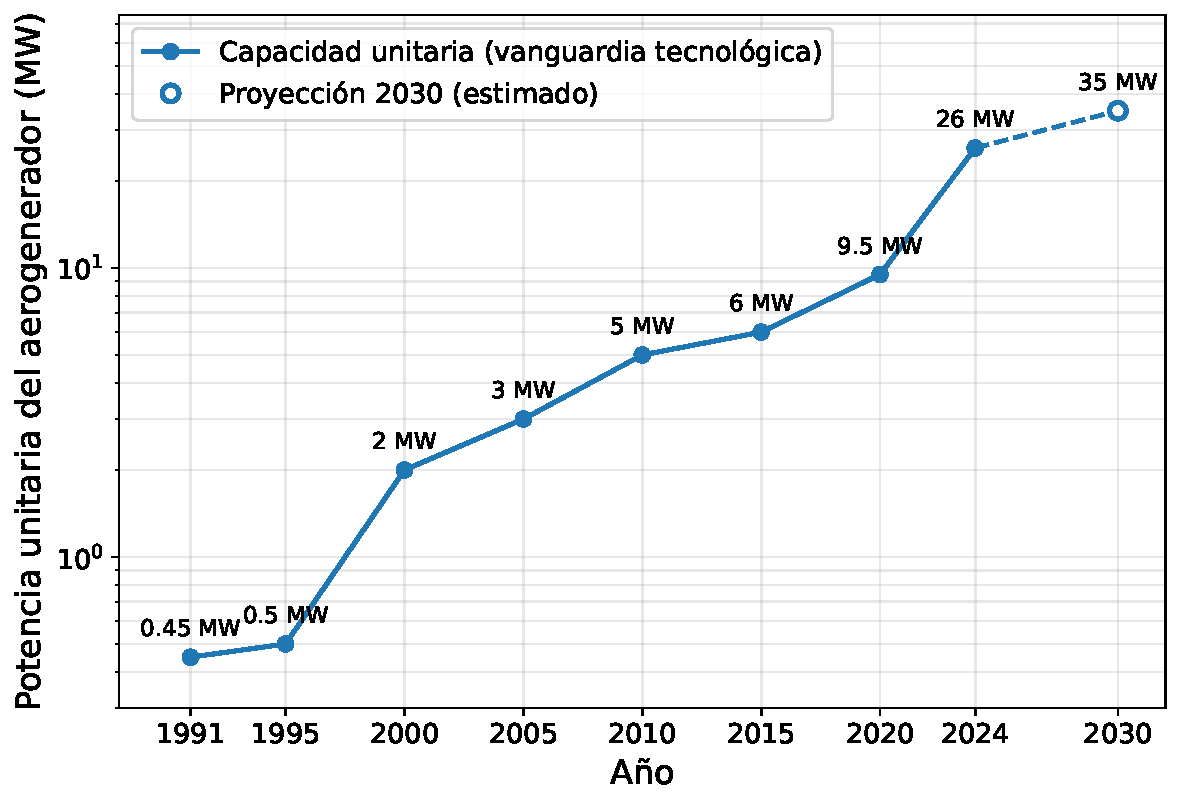
\includegraphics[width=0.75\textwidth]{Figuras/Figuras Antecedentes/crecimiento_turbinas_offshore.pdf}
    \caption[Crecimiento de la potencia unitaria de aerogeneradores offshore, 1991--2030.]{Crecimiento de la potencia unitaria de aerogeneradores offshore, 1991--2030. Elaboración propia a partir de los datos de \textcite{GWEC2025}.}
    \label{fig:crecimiento_turbinas}
\end{figure}

La densidad de potencia no es el único criterio relevante: también importa con qué frecuencia el viento se mantiene dentro del rango en que la turbina opera con eficiencia, aspecto que recoge el factor de planta, definido como el cociente entre la energía efectivamente generada en un periodo y la que se obtendría operando de forma continua a potencia nominal durante ese mismo periodo. En tierra, la turbulencia introducida por el relieve y los obstáculos vuelve el viento más irregular y reduce este valor incluso en las mejores zonas: esa misma franja de Chile central, de mayor recurso eólico terrestre del país, alcanza en el mar factores de planta de entre $40\%$ y $60\%$, superando el $70\%$ hacia el extremo sur~\parencite{Mattar2017}. A escala global, la flota offshore opera con un factor de planta medio ponderado del $41\%$~\parencite{GWEC2025}, cifra que ha llevado a organismos como la Agencia Internacional de Energía a describir la eólica marina como una tecnología de base variable, capaz de complementar el perfil diario y estacional de la generación solar~\parencite{GWEC2025}.

Este crecimiento no ha estado acompañado de un desarrollo equivalente de las bases científicas del diseño. Un grupo internacional de investigadores en energía eólica sistematizó, en la iniciativa \textit{Grand Challenges}, las brechas de conocimiento del sector en tres ámbitos críticos: la atmósfera, la turbina, y la planta junto a su interacción con la red~\parencite{Veers2022}. El segundo de ellos es el que enmarca directamente el presente trabajo. \textcite{Veers2022} señalan que el aumento de tamaño y flexibilidad de las máquinas modernas ha desplazado el diseño fuera del dominio en que fueron establecidos sus supuestos y sus herramientas de modelación, y que la evidencia experimental a gran escala disponible resulta insuficiente para validar los modelos y materiales empleados. Los mismos autores advierten, además, que el avance logrado hasta ahora se ha sustentado en soluciones de ingeniería que rodean esas brechas, apoyadas más en la experiencia acumulada que en la comprensión fundamental de los fenómenos, enfoque que ya no basta para sostener el ritmo de innovación requerido.

Estas brechas se acentúan en el entorno marino. El aprovechamiento del recurso en aguas profundas obliga a instalar la turbina sobre una plataforma flotante en lugar de anclarla directamente al fondo marino, de modo que la estructura queda sometida de forma simultánea al viento, al oleaje y a las corrientes, condiciones que definen el clima marino del emplazamiento y que se encuentran escasamente caracterizadas en comparación con las terrestres~\parencite{Veers2022}. A ello se suma que las nuevas máquinas deben ser, al mismo tiempo, mayores y más livianas para aprovechar ese recurso con eficiencia~\parencite{Veers2022}. La combinación de palas esbeltas con el movimiento de la plataforma traslada el punto crítico del diseño desde el rendimiento aerodinámico hacia la integridad estructural de componentes sometidos a cargas cíclicas de gran amplitud~\parencite{Borg2015}, y es en esa intersección, la verificación estructural de la pala bajo cargas aerodinámicas obtenidas conforme a la normativa vigente, donde se inscribe el presente trabajo.

\section{Potencial eólico offshore en Chile}

Chile posee un extenso borde costero y un potencial eólico marino que, según estudios del Banco Mundial~\parencite{BancoMundial2020}, supera los 957 GW, concentrado en la zona centro-sur y austral. El recurso es particularmente productivo hacia el extremo sur del país: en la franja entre los $45^\circ$ y $56^\circ$ S, que incluye la región de Magallanes, el factor de planta alcanza en gran medida valores superiores al $60\%$, llegando puntualmente al $70\%$~\parencite{Mattar2017}.

Este recurso se concentra mayoritariamente en zonas de alta profundidad donde las soluciones de cimentación fija no son viables: del potencial total, solo 131 GW corresponden a cimentación fija, mientras que la fracción más significativa, 826 GW, corresponde a las tecnologías flotantes, como se observa en la Figura~\ref{fig:potencial_offshore}~\parencite{BancoMundial2020}. Esta diferencia de escala sitúa a las plataformas flotantes como una alternativa viable para el aprovechamiento del recurso en el contexto nacional.

\begin{figure}[h]
    \centering
    %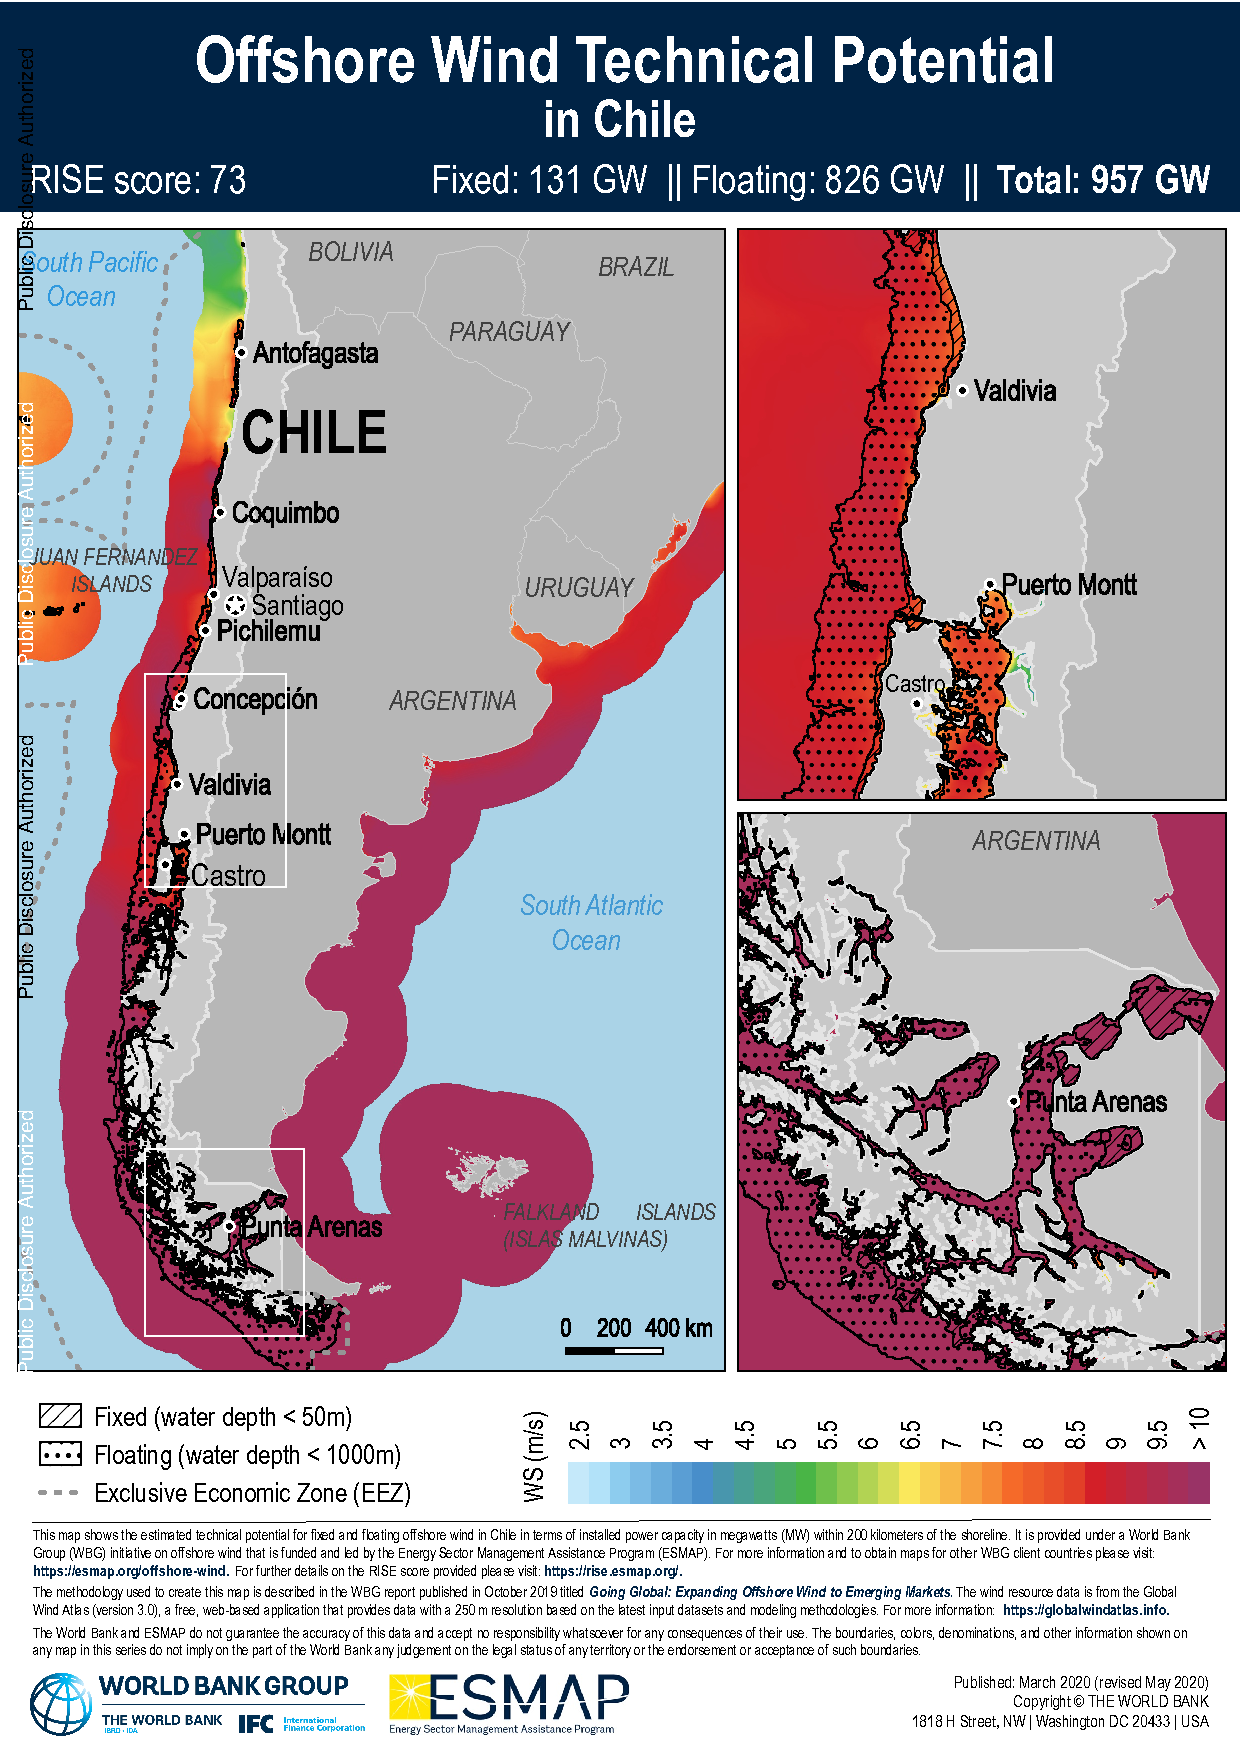
\includegraphics[width=0.75\textwidth]{Figuras/Technical-Potential-for-Offshore-Wind-in-Chile-Map.pdf}
    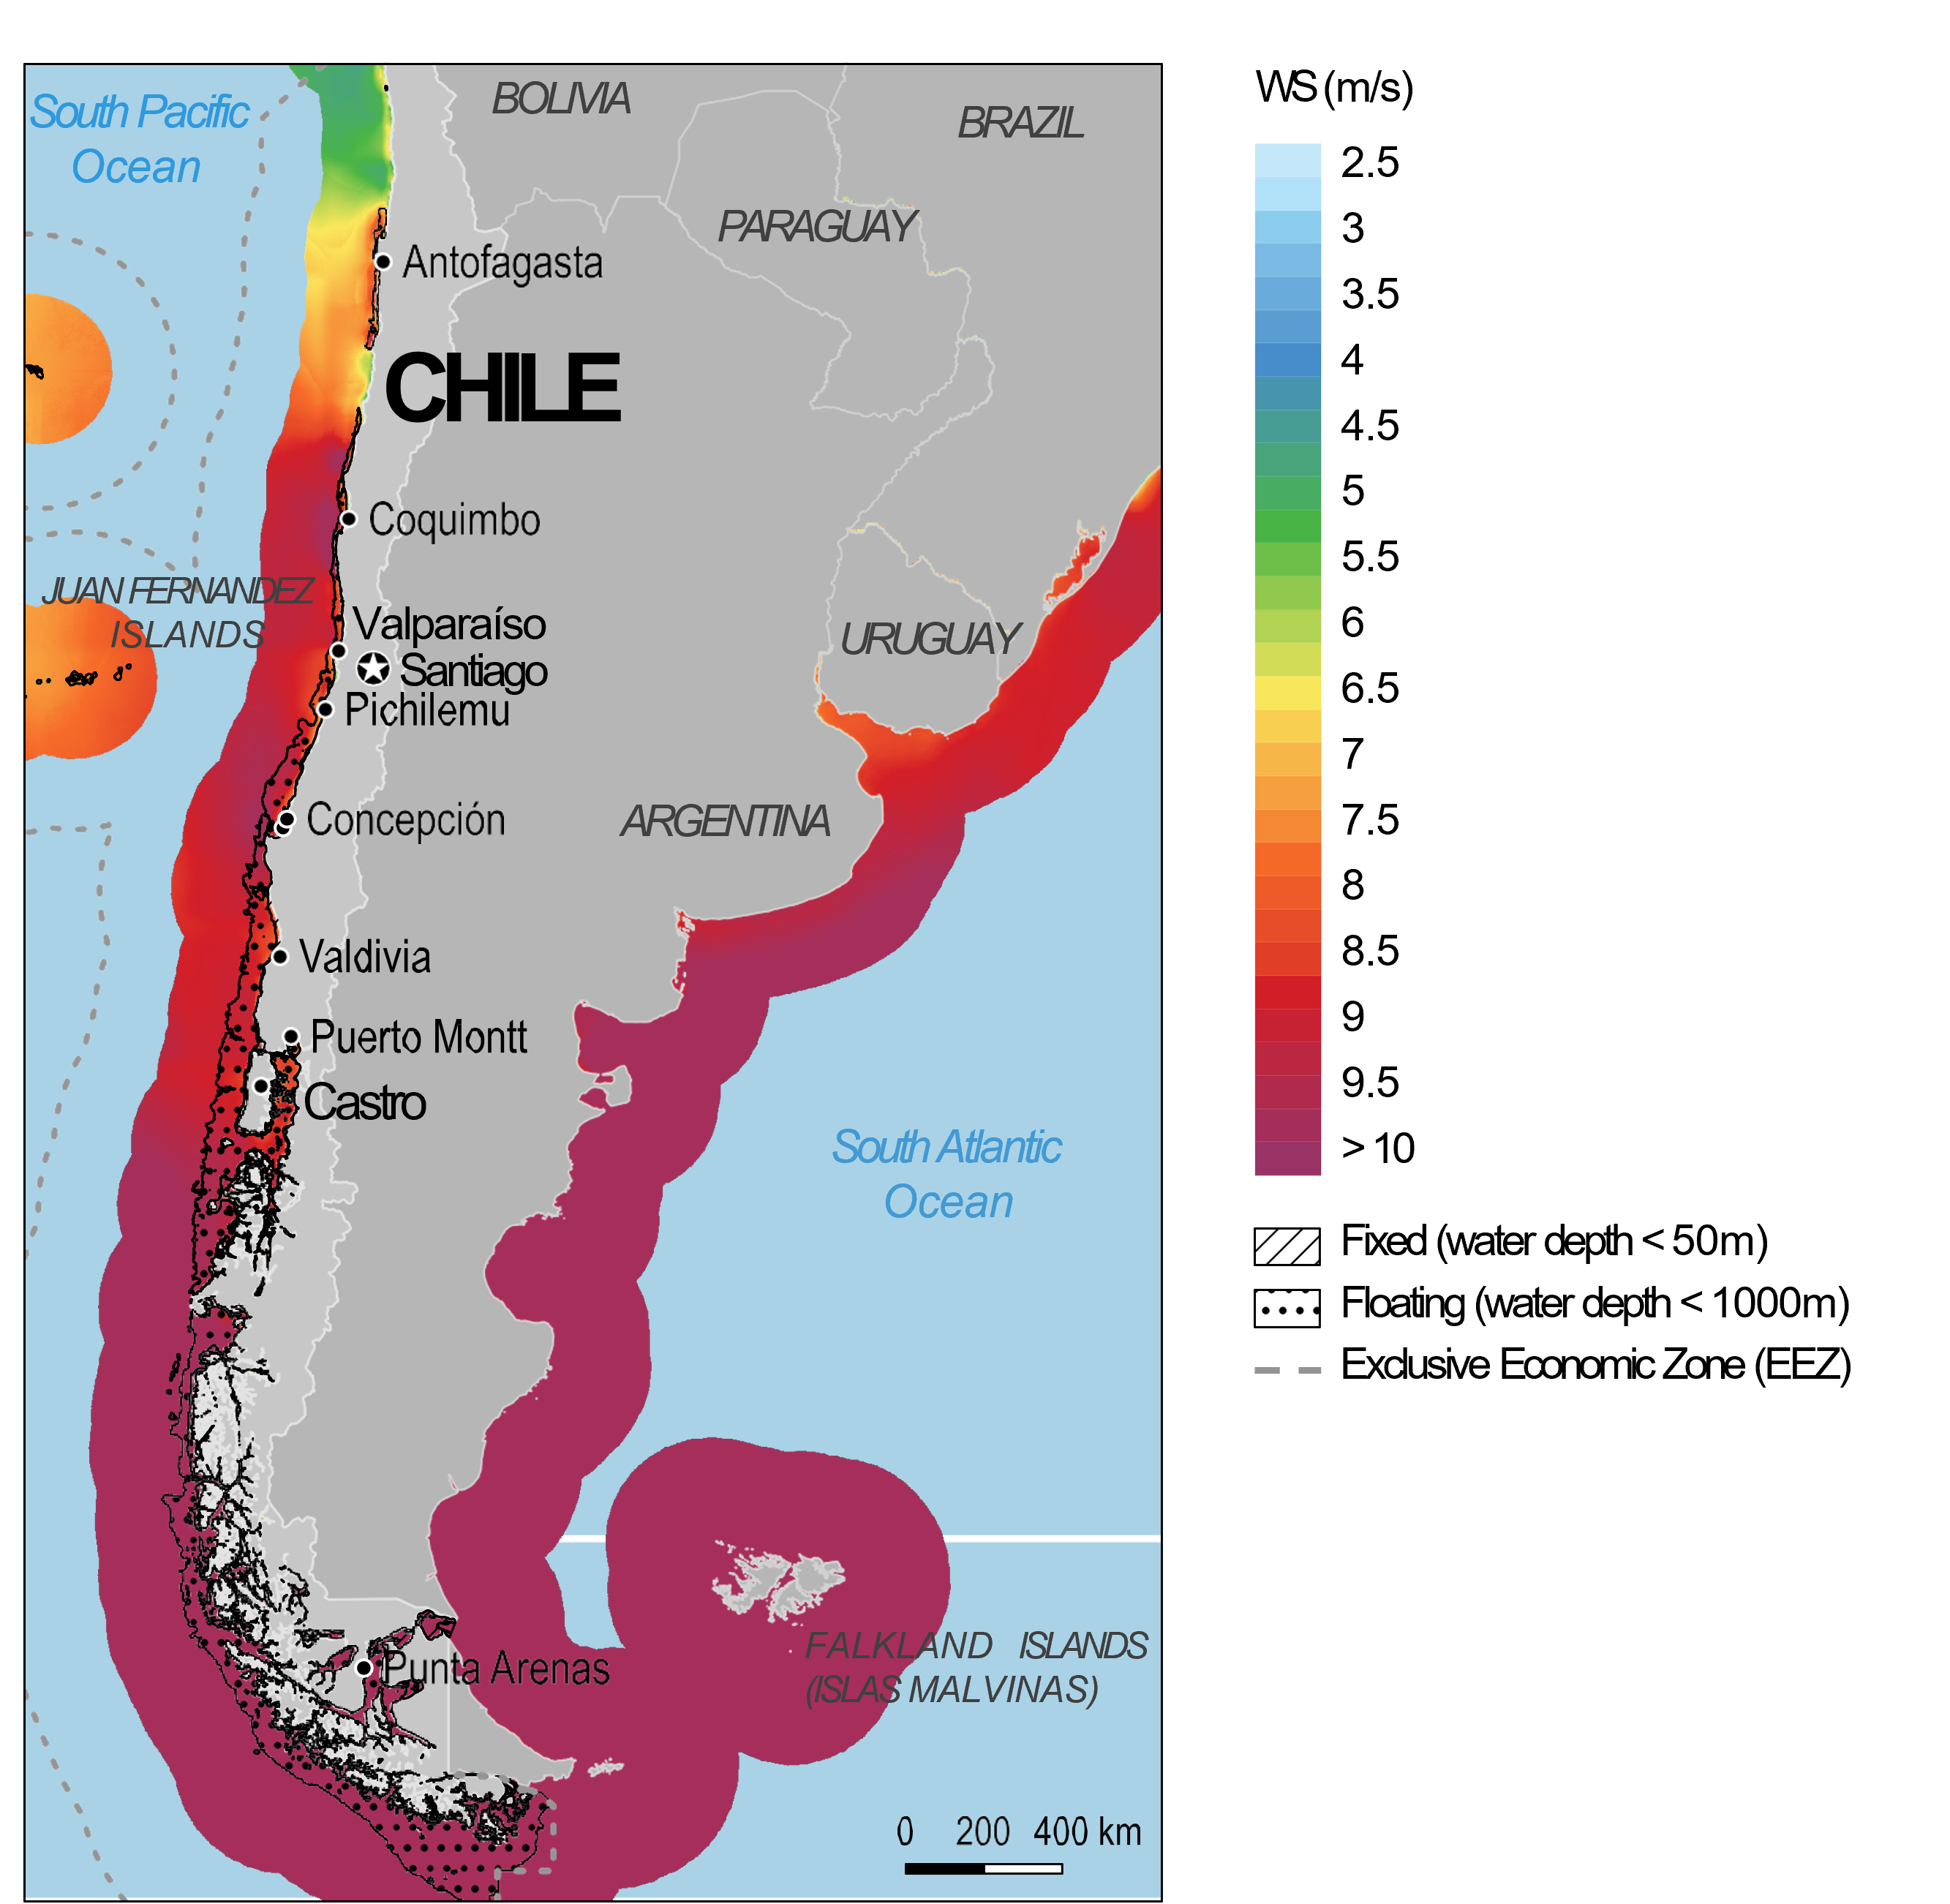
\includegraphics[width=0.75\textwidth]{Figuras/wind map.png}
    \caption[Modificado de potencial técnico de energía eólica marina en Chile.]{Modificado de potencial técnico de energía eólica marina en Chile~\parencite{BancoMundial2020}. La escala de color (WS) indica la velocidad media del viento (\textit{wind speed}); la fuente no especifica la altura de referencia a la que está evaluada.}
    \label{fig:potencial_offshore}
\end{figure}

\section{Tecnología offshore}
\label{sec:tecnologia-flotante}

El emplazamiento en el mar somete a la turbina a solicitaciones ausentes en tierra: a las cargas aerodinámicas se suman las condiciones de mar, cuyo efecto sobre el dimensionamiento estructural y sobre el análisis de fatiga resulta determinante~\parencite{Tampier2024}. En el caso de las estructuras flotantes, además, el oleaje induce movimientos de la plataforma que modifican la velocidad relativa del viento incidente sobre las palas y generan cargas inerciales adicionales~\parencite{Borg2015}. Estos efectos distinguen el diseño estructural offshore del terrestre y justifican la caracterización del recurso eólico bajo condiciones de turbulencia normal que se desarrolla en las secciones siguientes.

\subsection{Tipos de estructuras de soporte}

Las estructuras de soporte empleadas en el mar se agrupan en dos familias según su vínculo con el lecho marino, y la profundidad del emplazamiento es el criterio que determina cuál resulta aplicable, como se aprecia en la Figura~\ref{fig:tipos_estructuras}. Las estructuras fijas, solución dominante en la industria actual, transmiten las cargas directamente al lecho marino: el monopilote (\textit{monopile}), un cilindro de acero hincado en el fondo, cubre profundidades de 0 a 30 m, y la estructura reticulada tipo \textit{jacket} extiende el rango hasta los 25 a 60 m a costa de una mayor complejidad de fabricación; más allá de los 50 m, el volumen de material y las operaciones de instalación las vuelven económicamente inviables~\parencite{Tampier2024}.

A partir de esa profundidad se recurre a estructuras flotantes, ancladas mediante un sistema de fondeo y clasificadas según el mecanismo que provee la rigidez restauradora necesaria para limitar su inclinación~\parencite{Borg2015}: las estabilizadas por lastre, tipo \textit{spar}, concentran masa en su extremo inferior para situar el centro de gravedad muy por debajo del centro de la parte sumergida y operan desde los 120 m de profundidad; las estabilizadas por área de flotación, semisumergible o barcaza (\textit{barge}), obtienen el momento restaurador de la distribución horizontal de sus columnas o de su superficie de flotación y operan desde los 50 m; y las estabilizadas por fondeo, de piernas tensionadas (\textit{tension leg platform}), obtienen su rigidez de tirantes verticales pretensados anclados al fondo, que restringen fuertemente los movimientos verticales del conjunto~\parencite{Tampier2024,Borg2015}. Se estima que estos dispositivos podrán instalarse en profundidades de hasta 800 a 1\,000 m, si bien a la fecha el proyecto emplazado a mayor profundidad alcanza los 300 m~\parencite{Tampier2024}.

\begin{figure}[H]
    \centering
    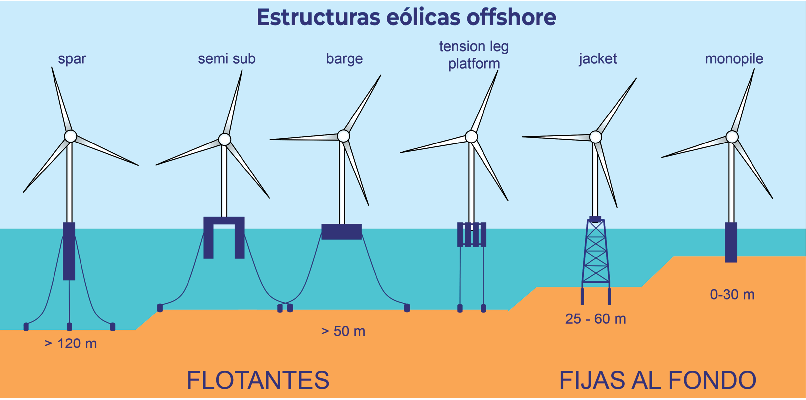
\includegraphics[width=0.85\textwidth]{Figuras/Figuras Antecedentes/estructuras_offshore.pdf}
    \caption[Estructuras eólicas offshore y profundidades típicas de instalación.]{Estructuras eólicas offshore y profundidades típicas de instalación~\parencite{Tampier2024}.}
    \label{fig:tipos_estructuras}
\end{figure}

\subsection{Retos del entorno flotante}
\label{sec:retos-flotante}

Mientras una torre terrestre se encuentra empotrada en el suelo, una plataforma flotante conserva seis grados de libertad de cuerpo rígido, definidos respecto de un sistema de coordenadas solidario a la estructura: tres desplazamientos, denominados \textit{surge} (longitudinal, en la dirección del viento), \textit{sway} (transversal) y \textit{heave} (vertical), y tres rotaciones, denominadas \textit{roll} (balanceo), \textit{pitch} (cabeceo) y \textit{yaw} (guiñada)~\parencite{Borg2015}. La Figura~\ref{fig:gdl_plataforma} ilustra esta convención.

\begin{figure}[H]
    \centering
    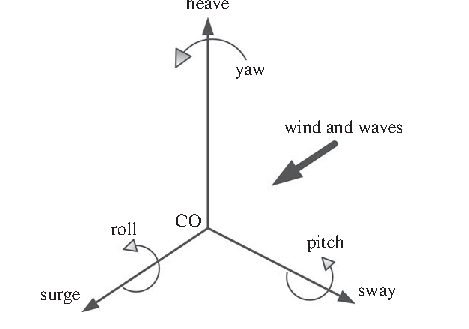
\includegraphics[width=0.55\textwidth]{Figuras/Figuras Antecedentes/gdl_plataforma.pdf}
    \caption[Grados de libertad de una plataforma eólica flotante.]{Grados de libertad de una plataforma eólica flotante respecto del centro de origen (CO)~\parencite{Borg2015}.}
    \label{fig:gdl_plataforma}
\end{figure}

De estos seis modos, el cabeceo es el que impone la restricción de diseño más severa, ya que el empuje aerodinámico del rotor actúa a gran altura sobre el centro de la parte sumergida y genera un momento de inclinación que la plataforma debe equilibrar. El diseño impone por ello un ángulo máximo de inclinación admisible, del cual se deriva la rigidez mínima que debe aportar la estructura de soporte: cuanto menor es el momento de inclinación que genera la turbina, menos costosa puede ser la subestructura~\parencite{Borg2015}.

A ello se suma un problema de acoplamiento dinámico. Las fuerzas aerodinámicas no solo desplazan la plataforma, sino que su carácter oscilatorio puede excitar sus modos propios de movimiento. \textcite{Borg2015} advierten que, en rotores de eje vertical de gran escala y baja velocidad de rotación, la frecuencia de paso de pala puede solaparse con el rango de frecuencias donde se concentra la energía del oleaje, condición que amplifica la respuesta del sistema y, con ella, la realimentación sobre la aerodinámica del rotor descrita al inicio de esta sección.

A estas restricciones se suma la orientación: una turbina de eje horizontal debe alinear activamente su rotor con la dirección del viento mediante un sistema de guiñada, que añade complejidad y masa en lo alto de la estructura, necesidad que desaparece en las configuraciones de eje vertical, insensibles a la dirección del viento incidente.

\subsection{Configuraciones de eje horizontal y de eje vertical}

Los aerogeneradores se clasifican según la orientación de su eje de rotación respecto del flujo incidente. En las turbinas eólicas de eje horizontal (HAWT, por sus siglas en inglés), el eje se dispone paralelo a la dirección del viento, de modo que el rotor debe orientarse activamente frente a él\glsunset{hawt}. Esta configuración domina las instalaciones de escala comercial, pero su despliegue está condicionado por el requerimiento de un flujo unidireccional y de baja turbulencia~\parencite{Essahraoui2026}.

En las turbinas eólicas de eje vertical (VAWT, por sus siglas en inglés), en cambio, el eje de rotación se dispone perpendicular a la componente horizontal del viento\glsunset{vawt}. De esta disposición se derivan sus propiedades características: la omnidireccionalidad, ya que el área barrida presenta la misma proyección con independencia de la dirección del viento, lo que elimina el sistema de guiñada y su hardware de control asociado; un centro de gravedad bajo, que simplifica las estructuras de soporte y las plataformas flotantes; una menor velocidad de punta; y una mayor tolerancia a la turbulencia~\parencite{Essahraoui2026}.

Dentro de la familia VAWT se distinguen a su vez las máquinas accionadas por arrastre, cuyo arquetipo es el rotor Savonius, y las accionadas por sustentación, correspondientes a las configuraciones Darrieus. Las primeras ofrecen un elevado torque de arranque y construcción simple, pero su coeficiente de potencia se limita a valores en torno a $0{,}25$; las segundas emplean perfiles alares y alcanzan coeficientes de potencia de $0{,}35$ a $0{,}45$ operando a relaciones de velocidad de punta mayores~\parencite{Essahraoui2026}.

Dentro de esas dos categorías, las configuraciones se diferencian por la forma y disposición de sus palas, según se representa en la Figura~\ref{fig:tipos_vawt}: el rotor Savonius, accionado por arrastre mediante palas acopadas; el H-Darrieus de pala recta; el Darrieus troposkeiano, de palas curvas que anulan la flexión bajo carga centrífuga; el Darrieus helicoidal, de palas retorcidas progresivamente en torno al eje para distribuir el torque a lo largo de la revolución; y las configuraciones híbridas, que acoplan un rotor Savonius interior a un Darrieus exterior para aprovechar su torque de arranque~\parencite{Essahraoui2026}.

\begin{figure}[H]
    \centering
    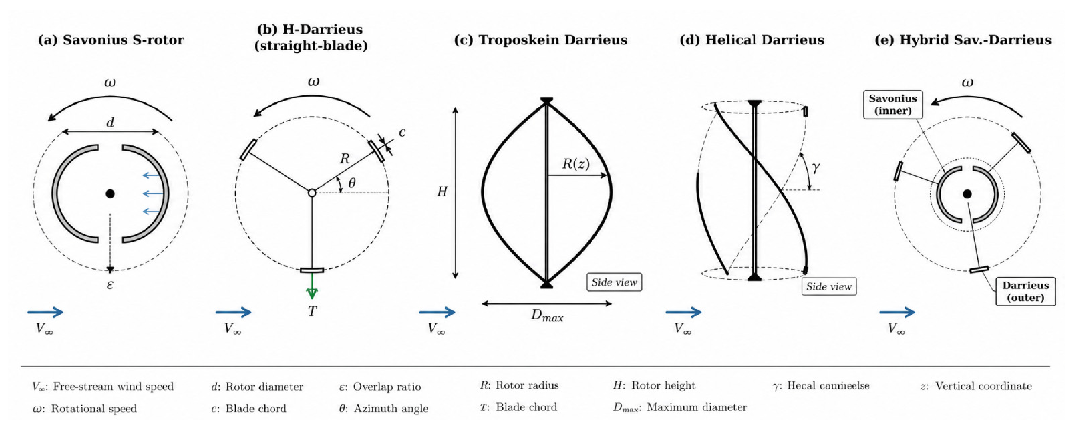
\includegraphics[width=\textwidth]{Figuras/Figuras Antecedentes/tipos_vawt.pdf}
    \caption[Configuraciones principales de VAWT.]{Configuraciones principales de VAWT~\parencite{Essahraoui2026}.}
    \label{fig:tipos_vawt}
\end{figure}

De todas ellas, el presente trabajo aborda una turbina tipo H-rotor, variante de pala recta de la familia Darrieus, cuyo análisis aerodinámico y estructural constituye el objetivo de esta memoria. Por este motivo, los antecedentes que se presentan a continuación se enfocan en las características de esta familia de VAWT y en su aplicación a plataformas flotantes offshore.

Aplicadas al entorno flotante, estas propiedades se traducen en ventajas concretas frente a la configuración de eje horizontal. Las \gls{vawt} permiten ubicar componentes pesados, como el generador y el tren de potencia, a menor altura que en las \gls{hawt}, lo que reduce el momento de inclinación de la plataforma y, con ello, la rigidez mínima que debe aportar la estructura de soporte~\parencite{Borg2015}. \textcite{ennis2018} cuantifican esta ventaja para un rotor Darrieus de 5 MW: las plataformas resultantes son más pequeñas y menos costosas que las de una HAWT flotante equivalente, debido principalmente al menor centro de gravedad y a los menores momentos de inercia del conjunto, si bien el rotor de baja velocidad y alto torque exige un tren de potencia de mayor masa. La omnidireccionalidad del rotor añade una ventaja frente a los casos de carga normados: ante un cambio extremo de dirección del viento, su operación no se ve alterada de forma apreciable, mientras que una HAWT pasaría a trabajar bajo flujo sesgado, esto es, con el viento incidiendo oblicuamente sobre el plano del rotor~\parencite{Galinos2015,HAND2021}.

La Figura~\ref{fig:vawt_hrotor} muestra la configuración general de la turbina H-rotor empleada como referencia para los análisis desarrollados en los capítulos siguientes.

\begin{figure}[H]
    \centering
    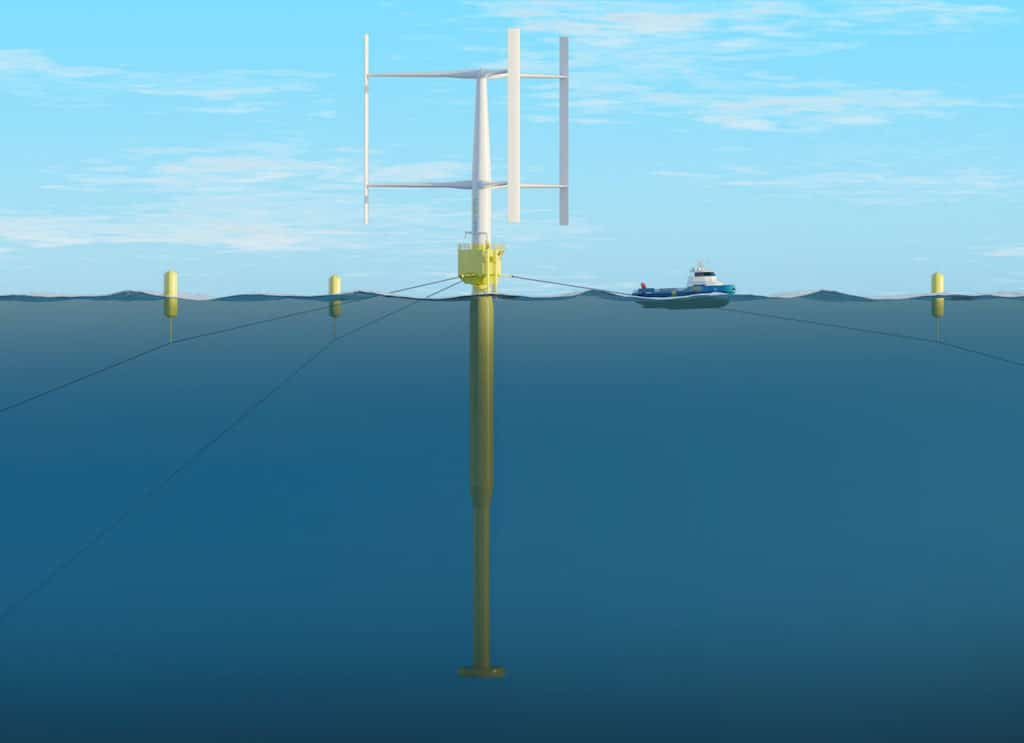
\includegraphics[width=0.6\textwidth]{Figuras/SeaTwirl_flotante.jpg}
    \caption[Configuración de aerogenerador de eje vertical tipo H-rotor.]{Configuración de aerogenerador de eje vertical tipo H-rotor empleada como caso de estudio~\parencite{SeaTwirl2026}.}
    \label{fig:vawt_hrotor}
\end{figure}

A diferencia de las turbinas de eje horizontal, cuyas cargas aerodinámicas presentan variaciones relativamente suaves durante la operación nominal, las VAWT en plataformas flotantes introducen desafíos de diseño propios: cada pala experimenta cambios periódicos en el ángulo de ataque y atraviesa repetidamente la estela generada por el propio rotor, mecanismos que dominan el campo de flujo y que los modelos cuasi-estacionarios no logran resolver~\parencite{Essahraoui2026}. En consecuencia, la determinación de las cargas de diseño requiere modelos aerodinámicos transitorios de mayor fidelidad~\parencite{Galinos2015}, constituyendo el punto de partida para analizar los principios aerodinámicos.

\section{Principios aerodinámicos de las VAWT}
\label{sec:aerodinamica}

\subsection{Geometría y partes del rotor}
\label{sec:geometria-rotor}

Un H-rotor está formado por un eje vertical, del cual se desprenden radialmente los brazos de soporte o \textit{struts}, y por un número $N$ de palas rectas de perfil alar montadas en el extremo de dichos brazos, dispuestas paralelas al eje de rotación. Esta disposición define las tres magnitudes geométricas que gobiernan el comportamiento del rotor, representadas en la Figura~\ref{fig:parametros_hrotor}:

\begin{itemize}
    \item El \textbf{radio del rotor} ($R$) es la distancia entre el eje de rotación y el plano medio de la pala. Corresponde al radio de la circunferencia que describe la pala al girar, y es la mitad del diámetro $D$ del rotor.
    \item La \textbf{altura de pala} ($H$) es la longitud de la pala medida en la dirección del eje de rotación.
    \item La \textbf{cuerda} ($c$) es la longitud de la sección transversal del perfil alar, medida sobre la línea recta que une su borde de ataque con su borde de fuga.
\end{itemize}

\begin{figure}[H]
    \centering
    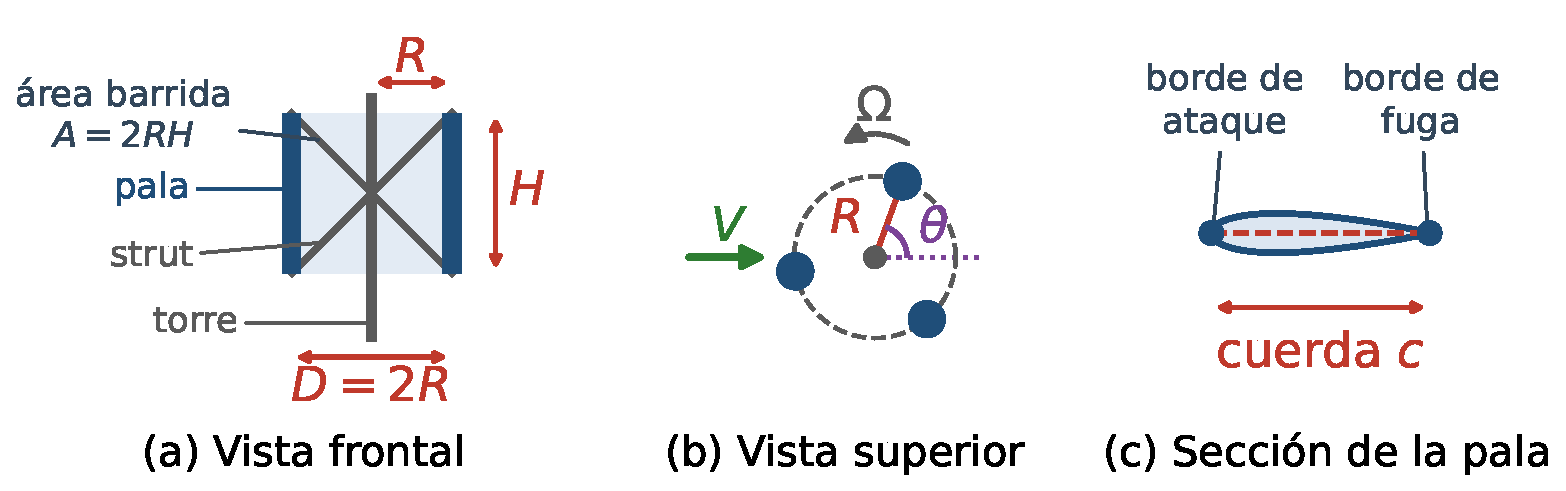
\includegraphics[width=\textwidth]{Figuras/Figuras Antecedentes/parametros_hrotor.pdf}
    \caption[Parámetros geométricos de un H-rotor.]{Parámetros geométricos de un H-rotor: radio $R$, diámetro $D$, altura de pala $H$, área barrida $A$, posición acimutal $\theta$ y cuerda $c$ de la sección. Elaboración propia.}
    \label{fig:parametros_hrotor}
\end{figure}

A diferencia de una \gls{hawt}, cuyo rotor barre un disco de área $\pi R^2$, el H-rotor barre la superficie lateral de un cilindro. El área proyectada frente al viento, que es la que interviene en los coeficientes adimensionales, corresponde por tanto al rectángulo de altura $H$ y ancho $D = 2R$, según la Ec.~\ref{eq:area_barrida}:

\begin{equation}
    A = 2RH
    \label{eq:area_barrida}
\end{equation}

Al girar, cada pala recorre una trayectoria circular sobre un plano horizontal. Su ubicación instantánea en dicha trayectoria se identifica mediante la \textbf{posición acimutal} ($\theta$), medida desde la dirección del viento incidente. La velocidad del viento se evalúa a la altura del centro del área barrida ($z_{hub}$), que en un H-rotor de palas rectas coincide con el punto medio de la pala, y la velocidad correspondiente a esa cota se denota $V_{hub}$. El subíndice conserva la notación de la norma IEC 61400-1, heredada de las \gls{hawt}, donde esa altura es la del buje que sostiene el rotor; en una VAWT no existe un elemento equivalente, por lo que la norma prescribe caracterizar las variables de viento a la altura del centro del área barrida~\parencite{IEC61400-1}.

La particularidad física del rotor de eje vertical reside en que la pala se desplaza alternadamente a favor y en contra del viento a lo largo de una misma revolución. En consecuencia, la velocidad relativa que percibe el perfil y el ángulo con que el flujo lo aborda varían de forma continua durante el giro, en contraste con una \gls{hawt}, donde ambas magnitudes permanecen aproximadamente constantes en operación nominal. De esta cinemática se derivan los parámetros que se definen a continuación.

\subsection{Parámetros adimensionales}

El rendimiento aerodinámico y las cargas sobre una turbina tipo H-rotor están gobernados por la interacción entre la velocidad del viento y la velocidad de rotación del sistema. Esta interacción se caracteriza mediante la relación de velocidad de punta (TSR, por sus siglas en inglés), que se define como la velocidad tangencial de la punta de la pala sobre la velocidad del viento, según la Ec.~\ref{eq:tsr}\glsunset{tsr}:

\begin{equation}
    \lambda = \frac{\Omega R}{V_{hub}}
    \label{eq:tsr}
\end{equation}

donde:
\begin{itemize}
    \item $\Omega$ es la velocidad angular de rotación (rad/s).
    \item $R$ es el radio del rotor (m).
    \item $V_{hub}$ es la velocidad del viento a la altura del centro del área barrida (m/s).
\end{itemize}

Para caracterizar el rendimiento del rotor se definen los coeficientes adimensionales de potencia ($C_p$) y de momento o torque ($C_m$), presentados en las Ecs.~\ref{eq:cp} y~\ref{eq:cm}, que expresan qué fracción de la potencia disponible en el flujo aprovecha la turbina y qué torque desarrolla, respectivamente:

\begin{equation}
    C_p = \frac{P}{\frac{1}{2}\rho A V_{hub}^3}
    \label{eq:cp}
\end{equation}

\begin{equation}
    C_m = \frac{M}{\frac{1}{2}\rho A R V_{hub}^2}
    \label{eq:cm}
\end{equation}

donde:
\begin{itemize}
    \item $P$ es la potencia mecánica generada.
    \item $M$ es el torque aerodinámico.
    \item $\rho$ es la densidad del fluido.
    \item $A = 2RH$ es el área barrida por el rotor, definida en la Ec.~\ref{eq:area_barrida}.
\end{itemize}

Ambos coeficientes no son independientes, sino que se relacionan a través de la relación de velocidad de punta mediante $C_p = \lambda C_m$~\parencite{Essahraoui2026}.

\subsection{Cinemática de la pala y ángulo de ataque}
\label{sec:cinematica}

La velocidad que percibe el perfil no es la del viento incidente, sino la \textbf{velocidad relativa} ($W$), resultante de componer la velocidad del viento con la velocidad tangencial de la pala. El \textbf{ángulo de ataque} ($\alpha$) es el ángulo formado entre la cuerda del perfil y la dirección de esa velocidad relativa, y es la variable que gobierna las fuerzas aerodinámicas sobre la pala. La Figura~\ref{fig:top_view} muestra el triángulo de velocidades que define ambas magnitudes en la vista superior del rotor.

\begin{figure}[H]
    \centering
    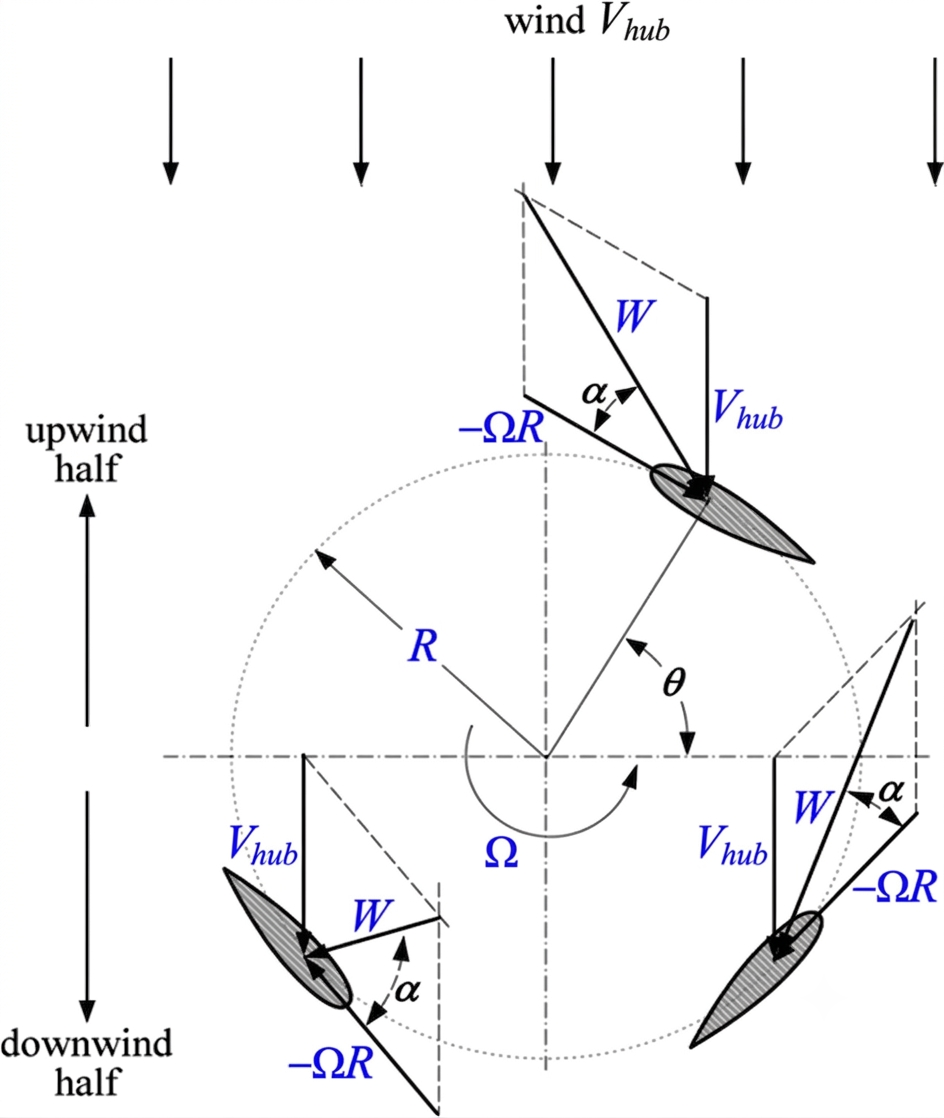
\includegraphics[width=0.5\textwidth]{Figuras/top_view_VAWT.png}
    \caption[Cinemática del H-rotor y triángulo de velocidades.]{Cinemática del H-rotor y triángulo de velocidades. El producto $\Omega R$ es la velocidad tangencial de la pala; el signo negativo indica que se compone en sentido opuesto a su avance. Modificado de \textcite{Tchakoua2015}.}
    \label{fig:top_view}
\end{figure}

En una \gls{hawt} el ángulo de ataque se mantiene relativamente constante en condiciones nominales. En un H-rotor, en cambio, la pala recorre posiciones a favor y en contra del viento dentro de una misma revolución, por lo que $\alpha$ experimenta una variación cíclica severa en función de la posición acimutal ($\theta$). Para un rotor de palas rectas, la cinemática básica define este ángulo según la Ec.~\ref{eq:alpha_theta}:

\begin{equation}
    \alpha(\theta) = \tan^{-1}\left(\frac{\sin\theta}{\lambda + \cos\theta}\right)
    \label{eq:alpha_theta}
\end{equation}

donde:
\begin{itemize}
    \item $\theta$ es la posición acimutal de la pala, medida desde la dirección del viento incidente.
    \item $\lambda$ es la relación de velocidad de punta definida en la Ec.~\ref{eq:tsr}.
\end{itemize}

Esta variación cíclica induce fluctuaciones en las cargas aerodinámicas durante cada revolución~\parencite{Bianchini2015,Borg2015}, fenómeno dominado por la pérdida dinámica que se describe en la Sección~\ref{sec:dynamicstall}.

\subsection{Solidez del rotor}
\label{sec:solidez}

La solidez ($\sigma$) relaciona la superficie total de pala con el área barrida. Para un H-rotor de $N$ palas de cuerda $c$ y radio $R$, se define según la Ec.~\ref{eq:solidez}:

\begin{equation}
\sigma = \frac{Nc}{R}
\label{eq:solidez}
\end{equation}

Este parámetro controla la posición del máximo de $C_p$ en función del TSR: rotores de baja solidez ($\sigma < 0{,}2$) operan a TSR elevados ($\lambda > 4$) con menor interferencia pala-estela, pero presentan pobre capacidad de autoarranque; rotores de alta solidez ($\sigma > 0{,}4$) alcanzan su máxima eficiencia a TSR bajos ($\lambda \approx 2\text{--}3$) y ofrecen mayor torque de arranque, a costa de una interacción pala-estela más intensa~\parencite{Essahraoui2026}.

Conviene advertir que la literatura emplea dos convenciones para esta magnitud. La adoptada en este trabajo, $\sigma = Nc/R$, es la de \textcite{Essahraoui2026}, mientras que otros autores la refieren al diámetro del rotor, $\sigma_d = Nc/d$~\parencite{Rezaeiha2018,Miller2021}, definición que para una misma geometría arroja la mitad del valor anterior. Cualquier contraste de solidez con datos de la literatura exige, por tanto, verificar previamente cuál de las dos definiciones emplea la fuente.

\subsection{Velocidad de punta y carga centrífuga}
\label{sec:vtip}

Sobre la pala en operación actúan tres tipos de carga: las aerodinámicas, las gravitatorias y las centrífugas, siendo estas dos últimas de naturaleza inercial y de carácter estacionario mientras la velocidad de rotación se mantenga constante~\parencite{Galinos2015}. Al describir la pala una trayectoria circular, la aceleración centrífuga a que queda sometida crece con el cuadrado de la velocidad de punta ($V_{tip} = \Omega R$), según la Ec.~\ref{eq:centrifugal_limit}:

\begin{equation}
    a_c = \Omega^2 R = \frac{V_{tip}^2}{R}
    \label{eq:centrifugal_limit}
\end{equation}

donde:
\begin{itemize}
    \item $a_c$ es la aceleración centrífuga en la punta de la pala, entendida como la fuerza inercial por unidad de masa que, en el marco de referencia solidario al rotor, actúa sobre la pala en dirección radial saliente. Su magnitud coincide con la de la aceleración centrípeta que describe el movimiento circular de la pala observado desde un marco fijo.
    \item $\Omega$ es la velocidad angular del rotor.
    \item $R$ es el radio del rotor.
\end{itemize}

El peso estructural de esta solicitación depende de la configuración del rotor. En un Darrieus de palas curvas la pala queda solicitada únicamente a tracción y sus tensiones de flexión radial resultan prácticamente nulas durante la operación, escenario particularmente favorable para un material compuesto~\parencite{Sutherland2012}. El H-rotor renuncia a esa condición a cambio de un radio constante: sus palas rectas, paralelas al eje de rotación, reciben la carga centrífuga en dirección perpendicular a su envergadura, que actúa como una carga transversal distribuida y las flecta entre sus puntos de unión a los struts, por lo que sus momentos flectores resultan mayores que en la configuración de palas curvas~\parencite{Mollerstrom2019}.

La velocidad de punta, por sí sola, no permite comparar máquinas de distinto tamaño. La Ec.~\ref{eq:centrifugal_limit} muestra que, para una misma velocidad de punta, la aceleración centrífuga es inversamente proporcional al radio: un rotor grande alcanza esa velocidad girando lentamente y con una solicitación moderada, mientras que uno pequeño debe girar mucho más rápido para lograrla y queda sometido a una solicitación mayor.

\subsection{Regímenes de operación y velocidad de rotación}
\label{sec:regimenes_operacion}

El coeficiente de potencia de un rotor depende de la relación de velocidad de punta (Ec.~\ref{eq:tsr}), de modo que aprovechar al máximo la energía disponible exige que la máquina permanezca en el $\lambda$ de mayor eficiencia. Como la velocidad del viento varía de forma continua, sostener esa condición obliga a que la velocidad de rotación la acompañe. La exigencia se acentúa en viento turbulento, condición en la que el \gls{tsr} óptimo de una \gls{vawt} de $200$~kW se desplaza respecto del que se obtiene en flujo uniforme~\parencite{Mollerstrom2016}.

La velocidad de rotación que sostiene un $\lambda$ dado para cada velocidad de viento se obtiene despejando la propia definición de la relación de velocidad de punta, según se desarrolla en la Sección~\ref{sec:criterio_rotacion}. Esa relación gobierna la operación por debajo de la velocidad de viento nominal, el régimen en que la turbina extrae la máxima energía disponible y en el que el $\lambda$ se mantiene constante en su valor de diseño.

Por encima de esa velocidad la relación deja de aplicarse, ya que continuar acelerando el rotor llevaría la velocidad de punta, y con ella la carga centrífuga de la Sección~\ref{sec:vtip}, más allá del límite admisible. La velocidad de rotación se mantiene entonces en su valor máximo y el \gls{tsr} decae a medida que el viento arrecia, con la consiguiente pérdida de coeficiente de potencia. La velocidad de viento que separa ambos regímenes queda determinada por la geometría del rotor y por ese límite de rotación, sin depender de ninguna magnitud ajena a ellos.

\subsection{Pérdida aerodinámica: del régimen estático al dinámico}
\label{sec:dynamicstall}

La pérdida aerodinámica, o \textit{stall}, es el fenómeno que fija el límite superior de la sustentación de un perfil y, en una \gls{vawt}, el que gobierna tanto la potencia extraída como las cargas cíclicas sobre la pala. Su descripción exige fijar previamente la nomenclatura del perfil alar, que se recoge en la Figura~\ref{fig:perfil_anatomia}.

\begin{figure}[H]
    \centering
    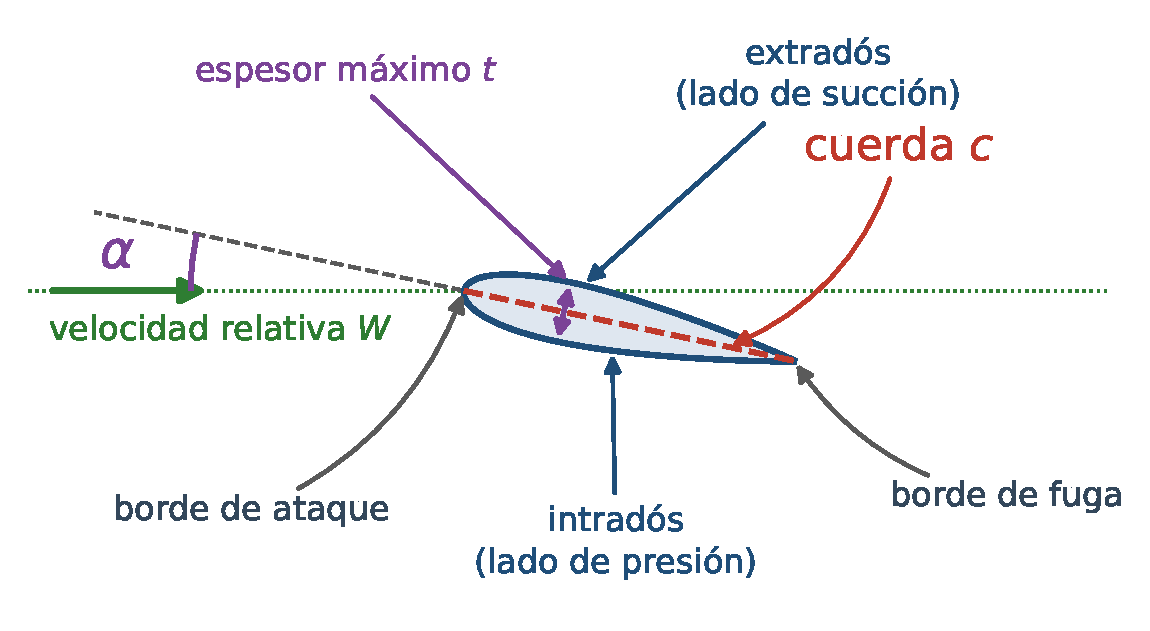
\includegraphics[width=0.82\textwidth]{Figuras/Figuras Antecedentes/perfil_anatomia.pdf}
    \caption{Nomenclatura del perfil alar y definición del ángulo de ataque.}
    \label{fig:perfil_anatomia}
\end{figure}

El borde de ataque es el extremo redondeado que enfrenta al flujo y el borde de fuga el extremo afilado opuesto. La recta que los une es la cuerda, de longitud $c$. La superficie superior, o extradós, es aquella sobre la cual el flujo se acelera y la presión disminuye, por lo que se denomina lado de succión; la inferior, o intradós, constituye el lado de presión. El espesor máximo $t$ caracteriza la esbeltez del perfil y, en la familia \gls{naca} de cuatro dígitos, se expresa como porcentaje de la cuerda. El ángulo de ataque $\alpha$ es el que forma la cuerda con la velocidad relativa $W$, según se definió en la Sección~\ref{sec:cinematica}.

La interacción entre el perfil y el flujo incidente produce una fuerza aerodinámica resultante que conviene descomponer respecto de la dirección de $W$: la sustentación es su componente perpendicular a $W$, y la resistencia (o arrastre), su componente paralela, en el sentido del flujo. Para comparar perfiles y condiciones de vuelo distintas, ambas se adimensionalizan dividiéndolas por la presión dinámica del flujo y el área de referencia, obteniéndose el coeficiente de sustentación $C_l$ y el coeficiente de resistencia $C_d$; de manera análoga se define el coeficiente de momento $C_m$, asociado al giro que la distribución de presiones induce sobre el perfil. Los tres dependen principalmente del ángulo de ataque $\alpha$ y, en menor medida, del número de Reynolds $Re$, razón entre las fuerzas inerciales y las viscosas del flujo, que caracteriza cuánto influye la viscosidad sobre su comportamiento. Las curvas de $C_l$, $C_d$ y $C_m$ en función de $\alpha$ para un $Re$ dado constituyen la polar aerodinámica del perfil, que se retoma con mayor detalle en la Sección~\ref{sec:polares}.

\subsubsection{Pérdida estática}

Sobre la superficie del perfil el aire no desliza libremente: la condición de adherencia impone velocidad nula en la pared, de modo que existe una región delgada, denominada capa límite, en la que la velocidad pasa de cero al valor del flujo exterior. Aguas abajo del punto de máxima succión el flujo debe recuperar presión, es decir, avanza contra un gradiente adverso de presión. Cuando ese gradiente es suficientemente intenso, el fluido de la capa límite, que ya ha perdido cantidad de movimiento por fricción viscosa, no logra continuar adherido y la capa límite se separa de la superficie.

La pérdida estática es la que se produce cuando el ángulo de ataque se incrementa lentamente. Al aumentar $\alpha$ crece la succión sobre el extradós y con ella el gradiente adverso, por lo que el punto de separación avanza progresivamente desde el borde de fuga hacia el de ataque, como ilustra la Figura~\ref{fig:stall_progresion}. Mientras el flujo permanece adherido, la sustentación crece de forma aproximadamente lineal con $\alpha$. Al alcanzarse el ángulo de pérdida estática $\alpha_{stall}$, la separación abarca ya una fracción sustancial del extradós: el coeficiente de sustentación alcanza su máximo $C_{l,max}$ y a partir de allí decae, mientras el coeficiente de arrastre aumenta con rapidez por efecto de la estela ancha que deja el perfil. La Figura~\ref{fig:stall_polar} recoge esta progresión sobre la polar del perfil \gls{naca}~0018.

\begin{figure}[H]
    \centering
    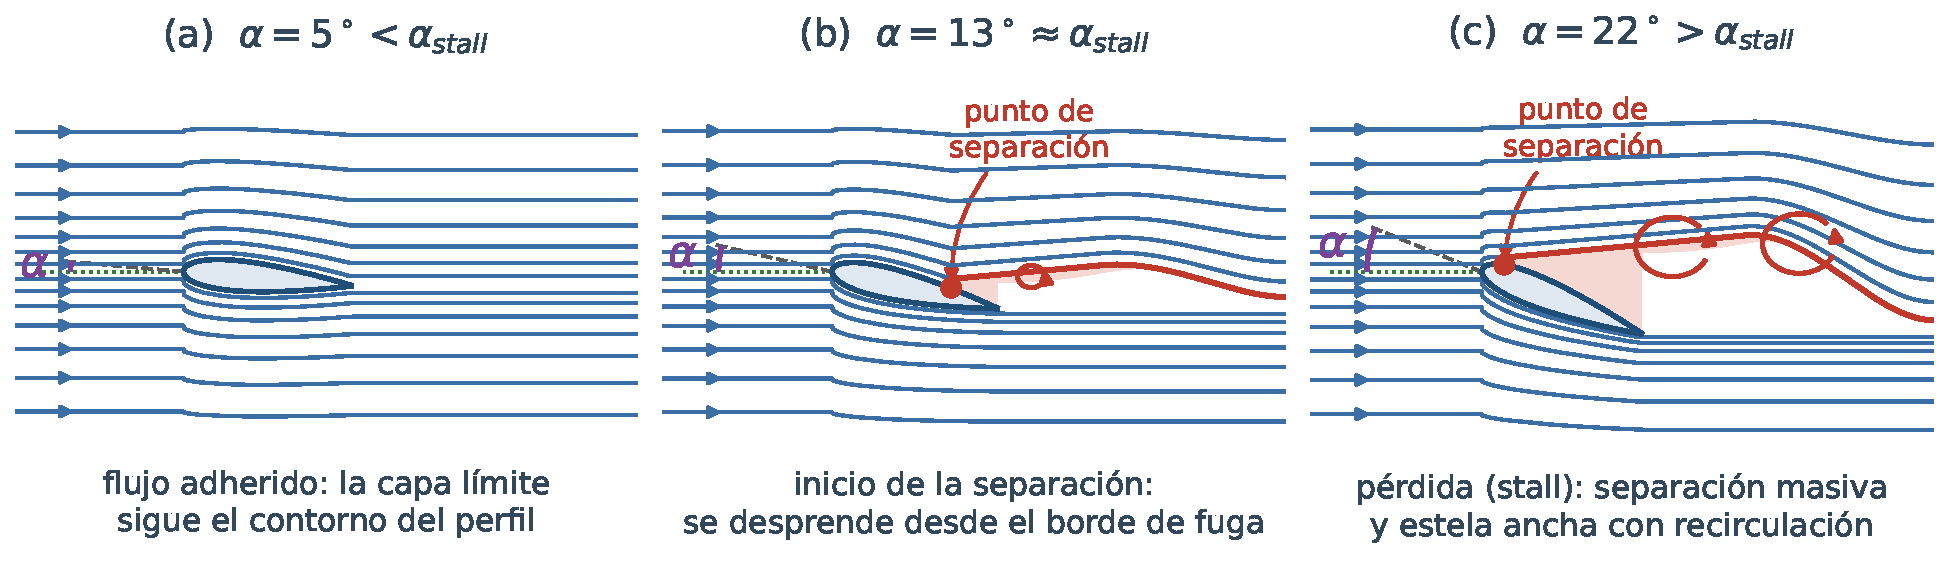
\includegraphics[width=\textwidth]{Figuras/Figuras Antecedentes/stall_progresion.pdf}
    \caption[Progresión de la separación de la capa límite con el ángulo de ataque.]{Progresión de la separación de la capa límite al aumentar el ángulo de ataque. La región sombreada indica la zona de flujo separado y las flechas circulares, la recirculación.}
    \label{fig:stall_progresion}
\end{figure}

\subsubsection{Pérdida dinámica}

Cuando el ángulo de ataque no varía lentamente sino con rapidez, como ocurre en la pala de una \gls{vawt} en cada revolución, la separación deja de seguir la secuencia estática. Durante la fase de aumento de $\alpha$ la capa límite permanece adherida más allá de $\alpha_{stall}$, retenida por la inercia del propio movimiento del flujo en las proximidades del borde de ataque, de modo que la sustentación continúa creciendo por encima de su máximo estático.

En esa condición se forma un vórtice de borde de ataque (LEV, por sus siglas en inglés)\glsunset{lev}, es decir, una concentración de vorticidad que nace del desprendimiento de la capa límite junto al borde de ataque y que permanece un tiempo sobre el extradós mientras crece. Al desplazarse sobre la superficie de succión induce una depresión adicional que se traduce en un exceso transitorio de sustentación, reportado en hasta un $50\%$ por encima del máximo estático~\parencite{Essahraoui2026}. Cuando el vórtice alcanza su tamaño límite se desprende y es arrastrado aguas abajo, momento en que la sustentación colapsa de forma abrupta, aparece flujo inverso sobre el extradós, esto es, una región donde el aire circula en sentido contrario al de la corriente principal, y el perfil entra en pérdida profunda.

Dado que la readherencia posterior del flujo ocurre a ángulos de ataque menores que aquel al que se produjo el desprendimiento, el ciclo de carga no es reversible: la curva $C_l$--$\alpha$ describe un lazo de histéresis, con sustentación superior a la estática durante el aumento de $\alpha$ e inferior durante su disminución~\parencite{Ferreira2009}. La carga real sobre la pala queda descrita por ese lazo y no por un valor único de $C_l$ para cada ángulo. La Figura~\ref{fig:stall_polar} contrasta ese lazo con la polar estática.

\begin{figure}[H]
    \centering
    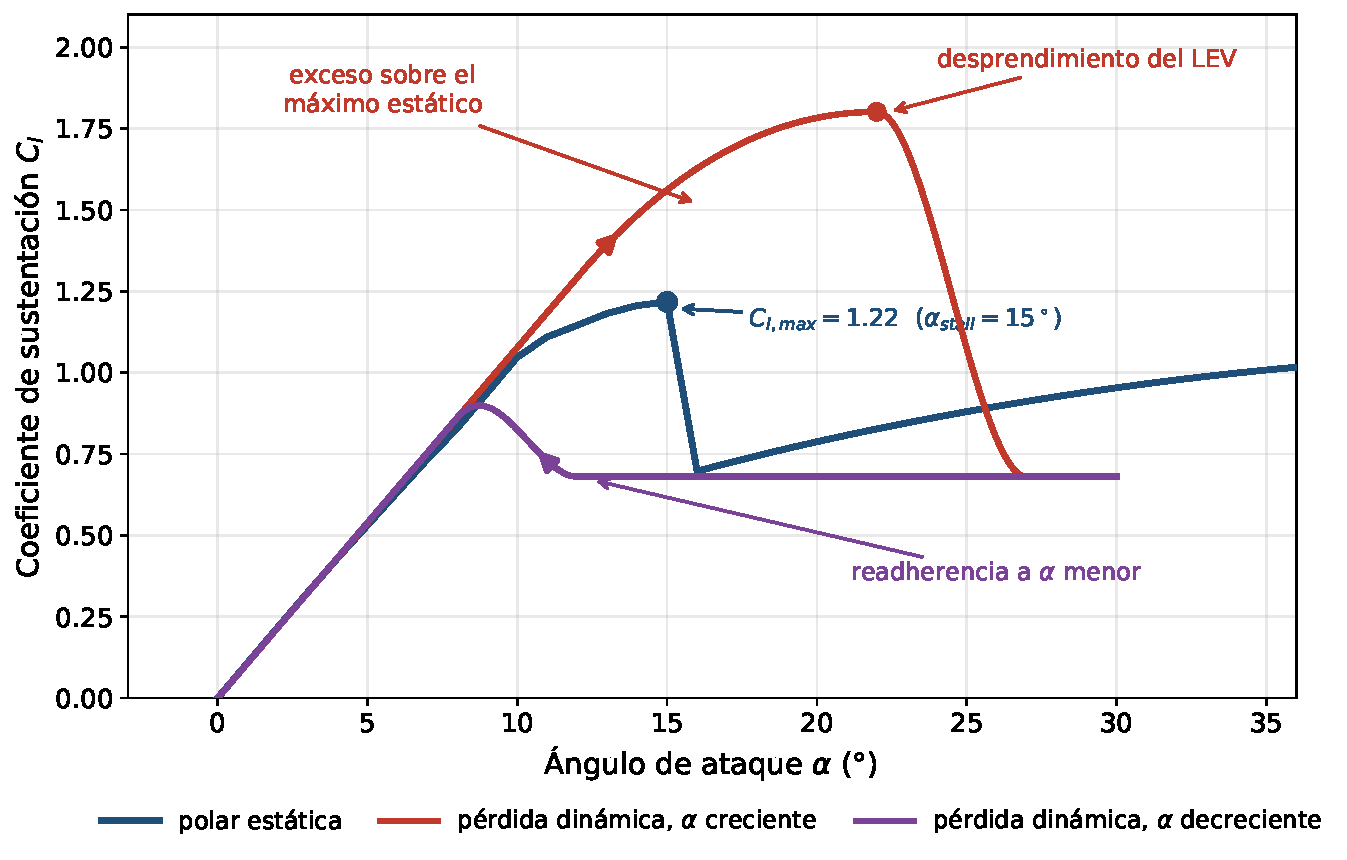
\includegraphics[width=0.8\textwidth]{Figuras/Figuras Antecedentes/stall_polar.pdf}
    \caption[Pérdida estática y dinámica del perfil NACA 0018.]{Pérdida estática y dinámica del perfil \gls{naca}~0018 a $Re = 1\times10^{6}$. La polar estática procede de las curvas calculadas para este trabajo; el lazo de histéresis es una representación cualitativa de la secuencia descrita en el texto, no una medición ni una simulación.}
    \label{fig:stall_polar}
\end{figure}

\subsubsection{Excursión del ángulo de ataque y su dependencia del TSR}

En un H-rotor la pala recorre una circunferencia mientras el viento sopla en una dirección fija, de manera que la posición acimutal $\theta$ determina la orientación relativa entre ambos. Se denomina semiciclo de barlovento a la mitad de la revolución en que la pala atraviesa el lado del rotor que enfrenta primero al viento, y semiciclo de sotavento a la mitad restante, en la cual la pala opera dentro de la estela generada por el propio rotor y encuentra, por tanto, un flujo ya frenado~\parencite{Essahraoui2026}.

El ángulo de ataque que percibe la pala queda determinado por la posición acimutal y por el \gls{tsr}, según la función $\alpha(\theta,\lambda)$ que expresa la Ec.~\ref{eq:alpha_theta}. Al derivar dicha expresión respecto de $\theta$ se obtiene que el extremo se alcanza en $\cos\theta = -1/\lambda$ y que su valor depende únicamente del \gls{tsr}, según la Ec.~\ref{eq:alpha_max}:

\begin{equation}
    \alpha_{max} = \arcsin\left(\frac{1}{\lambda}\right)
    \label{eq:alpha_max}
\end{equation}

La Ec.~\ref{eq:alpha_max} sintetiza el papel del \gls{tsr}: fijada la geometría, es la velocidad de rotación relativa a la del viento la que determina por sí sola la amplitud de la excursión angular. La Figura~\ref{fig:alpha_acimut} representa $\alpha(\theta)$ a lo largo de una revolución completa para tres valores de $\lambda$, junto con la banda en que el perfil se encuentra en pérdida.

\begin{figure}[H]
    \centering
    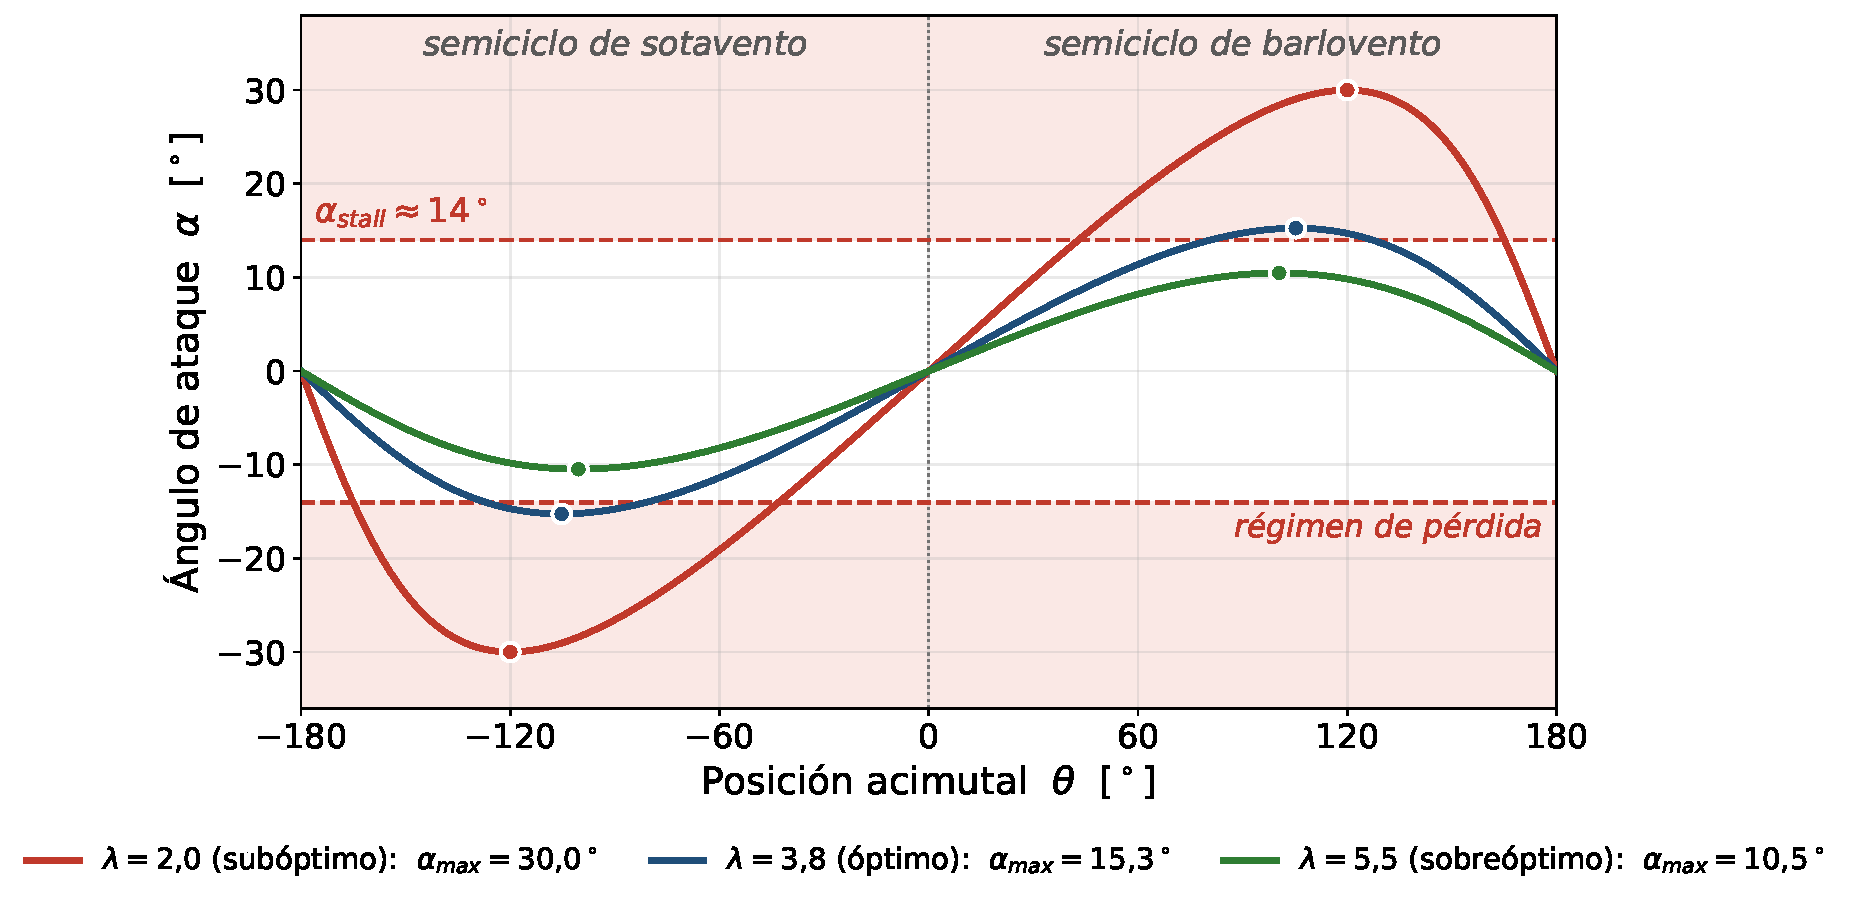
\includegraphics[width=0.92\textwidth]{Figuras/Figuras Antecedentes/alpha_acimut_tsr.pdf}
    \caption{Ángulo de ataque en función de la posición acimutal para tres \gls{tsr}.}
    \label{fig:alpha_acimut}
\end{figure}

La banda sombreada de la Figura~\ref{fig:alpha_acimut} corresponde al régimen de pérdida, delimitado por el ángulo de pérdida estática del perfil \gls{naca}~0018, que los ensayos en túnel de viento de \textcite{Bianchini2015} sitúan entre $14^\circ$ y $15^\circ$ para números de Reynolds de $1{,}5\times10^5$ a $3\times10^5$. Los puntos marcados sobre cada curva señalan los extremos que predice la Ec.~\ref{eq:alpha_max}. El contraste entre las tres ilustra el compromiso que fija el punto de operación: a $\lambda = 2$ la excursión alcanza $\alpha_{max} = 30^\circ$ y la pala atraviesa la banda de pérdida dos veces por revolución, una en cada semiciclo y con signos opuestos del ángulo de ataque; a $\lambda = 5{,}5$ el flujo permanece adherido durante todo el ciclo, pero el rotor opera lejos del máximo de sustentación y aumentan las pérdidas viscosas y la interferencia con la estela~\parencite{Essahraoui2026}. Entre ambos extremos, \textcite{Essahraoui2026} señalan que la restricción cinemática que fija el \gls{tsr} óptimo de una configuración es que la envolvente de ángulos de ataque permanezca acotada por el ángulo de pérdida estática.

Esta progresión cuenta con verificación experimental directa. \textcite{Ferreira2009} visualizaron mediante velocimetría de imágenes de partículas (PIV, por sus siglas en inglés)\glsunset{piv} el campo de flujo sobre la pala de un rotor Darrieus para $\lambda = 2$, $3$ y $4$: a $\lambda = 2$ registraron la formación del vórtice de borde de ataque, su desprendimiento y su posterior interacción con la pala en el semiciclo de sotavento, fenómenos que se atenúan a $\lambda = 3$ y desaparecen a $\lambda = 4$, donde los ángulos de ataque alcanzados ya no bastan para producir el enrollamiento. El máximo desarrollo del vórtice se observó, además, en la posición acimutal que predice la Ec.~\ref{eq:alpha_max}.

\subsubsection{Consecuencias sobre las cargas y la fatiga}

El efecto de esta cinemática sobre las cargas es doble. En primer lugar, el torque no es constante a lo largo de la revolución: en el semiciclo de barlovento la pala produce el pico principal de fuerza tangencial mientras $\alpha(\theta)$ se mantiene por debajo del ángulo de pérdida, en tanto que en el de sotavento, al operar sobre el flujo ya frenado por el propio rotor, genera un pico secundario de menor magnitud~\parencite{Essahraoui2026}. Con $N$ palas igualmente espaciadas el torque resultante oscila $N$ veces por revolución. Para configuraciones de dos y tres palas con flujo adherido, el cociente entre la variación pico a pico del torque y su valor medio se sitúa entre $0{,}5$ y $1{,}5$, y aumenta de forma pronunciada cuando aparece la pérdida dinámica, condición en que la forma de onda del torque se vuelve marcadamente no sinusoidal~\parencite{Essahraoui2026}.

En segundo lugar, y con consecuencias directas sobre el objeto de este trabajo, la pala queda sometida a un régimen de carga intrínsecamente cíclico. \textcite{Mollerstrom2019} constatan que los problemas de fatiga han sido recurrentes en los proyectos de \gls{vawt} documentados, y lo atribuyen a que la dirección de las fuerzas aerodinámicas sobre la pala cambia de manera continua durante cada revolución, lo que somete al material a tensiones cíclicas de gran amplitud y, dado que cada revolución aporta un ciclo, a recuentos de ciclos muy elevados a lo largo de la vida útil. Añaden que la operación a \gls{tsr} bajo, que en una turbina de paso fijo es la que corresponde a las velocidades de viento altas, introduce además la pérdida dinámica y vuelve aún más brusca la variación de las cargas, y precisan que una \gls{hawt} experimenta también tensiones cíclicas, pero en menor medida, pues con viento estable y baja turbulencia la fuerza aerodinámica dominante se mantiene relativamente constante.

Este historial admite, no obstante, una precisión importante. En la retrospectiva del programa de \gls{vawt} de los Laboratorios Nacionales Sandia, \textcite{Sutherland2012} atribuyen las fallas por fatiga de las décadas de 1970 a 1990 al empleo de palas extruidas en aluminio 6063-T5, material de pobres propiedades frente a la fatiga, y no al concepto en sí: sostienen que las \gls{vawt} no son intrínsecamente más propensas a la fatiga que las \gls{hawt}, y que con el conocimiento actual de las cargas es posible diseñar palas que las resistan de manera fiable. La exigencia, en cambio, se mantiene en toda su magnitud, ya que la pala debe soportar del orden de $10^9$ ciclos a lo largo de su vida de diseño, recuento para el cual las bases de datos de fatiga de los materiales siguen resultando escasas.

De ahí que la verificación de una pala de H-rotor no pueda limitarse a la resistencia última frente a la carga extrema, sino que deba incorporar la acumulación de daño por fatiga a lo largo de la vida de diseño, exigencia que la norma recoge mediante el \gls{fls} y que se aborda en la Sección~\ref{sec:analisis-estructural}.
\section{Referencias de contraste para el rotor en estudio}
\label{sec:referencias-contraste}

Las magnitudes definidas en la sección anterior permiten describir un rotor, pero no juzgar si los valores obtenidos para él son razonables. Esta sección reúne las referencias empíricas con que se contrastan los resultados del Capítulo~4: los rangos operacionales documentados para cada configuración de VAWT, los parámetros de máquinas H-rotor efectivamente construidas de escala comparable al caso de estudio, y los criterios con que pueden compararse rotores de distinto tamaño.

\subsection{Rangos operacionales por configuración}
\label{sec:configuraciones-vawt}


La Tabla~\ref{tab:tabla_vawt} resume los valores característicos de las familias de VAWT presentadas en la Figura~\ref{fig:tipos_vawt}. Su utilidad en este trabajo es servir de referencia de contraste: los valores de $C_{p,max}$ y de TSR obtenidos en el Capítulo 4 para la turbina en estudio deben situarse dentro del rango documentado para la columna H-Darrieus.

\begin{table}[H]
    \centering
    \caption[Parámetros característicos de las principales configuraciones de VAWT.]{Parámetros característicos de las principales configuraciones de VAWT~\parencite{Essahraoui2026}.}
    \label{tab:tabla_vawt}
    \begin{tabular}{lccccc}
        \hline
        \textbf{Parámetro} & \textbf{Savonius} & \textbf{H-Darrieus} & \textbf{Troposkein} & \textbf{Helical} & \textbf{Híbrido}\\
        \hline
        $\lambda$ típico & $0{,}7\text{--}1{,}5$ & $2\text{--}5$ & $2{,}5\text{--}5$ & $2{,}5\text{--}5$ & $1\text{--}3$\\
        $\sigma$ & --- & $0{,}15\text{--}0{,}45$ & $0{,}15\text{--}0{,}40$ & $0{,}20\text{--}0{,}40$ & $0{,}25\text{--}0{,}50$\\
        $C_{p,max}$ & $0{,}15\text{--}0{,}25$ & $0{,}35\text{--}0{,}42$ & $0{,}35\text{--}0{,}45$ & $0{,}30\text{--}0{,}40$ & $0{,}25\text{--}0{,}35$\\
        \hline
        \multicolumn{6}{p{0.95\textwidth}}{\footnotesize La misma fuente reporta $C_{p,max}$ de hasta $0{,}45$ para configuraciones H-Darrieus optimizadas.}
    \end{tabular}
\end{table}

\subsection{Turbinas H-rotor de referencia}
\label{sec:turbinas_referencia}

La Tabla~\ref{tab:hrotor_rpm} resume los parámetros de algunos de los H-rotor tripala de escala comparable construidos a la fecha.

\begin{table}[H]
    \centering
    \caption[Parámetros de turbinas H-rotor tripala de escala comparable.]{Parámetros de turbinas H-rotor tripala de escala comparable. Modificado de \textcite{Mollerstrom2019}.}
    \label{tab:hrotor_rpm}
    \begin{tabular}{lccccc}
        \hline
        \textbf{Turbina} & \textbf{D (m)} & \textbf{A (m$^2$)} & \textbf{Potencia nominal} & \textbf{$P/A$ (W/m$^2$)} & \textbf{Material de palas}\\
        \hline
        T1-turbine & 26{,}0 & 624 & 200 kW @ 12 m/s & 321 & Fibra de vidrio \\
        ANew-M1    & 24{,}0 & 360 & 200 kW @ 12 m/s & 556 & Vidrio y carbono \\
        Skwid      & 24{,}0 & 850\textsuperscript{*} & 500 kW @ 13 m/s & 588 & --- \\
        \hline
        \multicolumn{6}{p{0.92\textwidth}}{\footnotesize $P/A$: potencia específica. \textsuperscript{*}Área estimada en la fuente.}
    \end{tabular}
\end{table}

Las tres máquinas de la Tabla~\ref{tab:hrotor_rpm} son H-rotor tripala de eje vertical con generador de accionamiento directo y velocidad variable. La T1-turbine es un prototipo terrestre instalado en Falkenberg, Suecia (2010), con palas de fibra de vidrio; la ANew-M1, un prototipo terrestre emplazado cerca de Cracovia, Polonia (2015), con torre de acero y palas de fibra de vidrio y carbono; y la Skwid, un prototipo flotante offshore desarrollado en Japón (2013), que acoplaba el H-rotor a un rotor Savonius sumergido para el aprovechamiento de corrientes~\parencite{Mollerstrom2019}.

Al tratarse de máquinas efectivamente construidas y operadas, sus parámetros provienen de la experiencia y no de un ejercicio de diseño, y como comparten con el caso de estudio la configuración H-rotor tripala y un orden de magnitud equivalente en diámetro y área barrida, sus rangos de velocidad de rotación, \gls{tsr} y potencia específica delimitan el espacio de valores razonable para una máquina de esta familia y escala. De ellas, la T1-turbine es la que cuenta con más parámetros operacionales documentados en la literatura revisada, resumidos en la Tabla~\ref{tab:t1_params}.

\begin{table}[H]
    \centering
    \caption[Parámetros operacionales de la T1-turbine.]{Parámetros operacionales de la T1-turbine. Fuentes: (1)~\textcite{Mollerstrom2019}, (2)~\textcite{Mollerstrom2017}, (3)~\textcite{Mollerstrom2016}.}
    \label{tab:t1_params}
    \begin{tabular}{l c c}
        \hline
        \textbf{Parámetro} & \textbf{Valor} & \textbf{Fuente}\\
        \hline
        Diámetro del rotor            & $26$ m         & (1), (2)\\
        Longitud de pala              & $24$ m         & (1), (2)\\
        Velocidad de viento nominal   & $12$ m/s       & (1), (3)\\
        Velocidad de corte            & $25$ m/s       & (2), (3)\\
        \gls{tsr} objetivo            & $3{,}8$        & (2), (3)\\
        Velocidad de rotación         & $16$--$33$ rpm & (2), (3)\\
        \hline
    \end{tabular}
\end{table}

La Figura~\ref{fig:t1_turbine} muestra la T1-turbine instalada en Falkenberg. Se trata de un H-rotor de palas rectas, con tres palas de perfil alar dispuestas paralelas al eje de rotación y unidas a este mediante struts, de acuerdo con la configuración descrita en la Sección~\ref{sec:geometria-rotor}. Los tensores visibles en la imagen no forman parte del diseño original y fueron incorporados con posterioridad.

\begin{figure}[H]
    \centering
    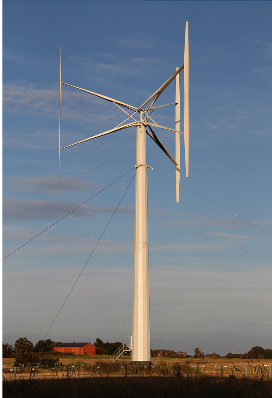
\includegraphics[width=0.42\textwidth]{Figuras/Figuras Antecedentes/t1_turbine.pdf}
    \caption[T1-turbine de 200 kW en Falkenberg, Suecia.]{T1-turbine de 200 kW en Falkenberg, Suecia~\parencite{Mollerstrom2019}.}
    \label{fig:t1_turbine}
\end{figure}

\subsection{Parámetros de comparación y velocidad de rotación de diseño}
\label{sec:criterio_rotacion}

La aceleración centrífuga de la Sección~\ref{sec:vtip} permite contrastar la severidad estructural de dos rotores de distinto radio, pero nada dice sobre su desempeño aerodinámico, comparación que se apoya en magnitudes normalizadas antes que en valores absolutos. Para las VAWT, \textcite{Essahraoui2026} identifican, junto al principio de operación, cuatro parámetros de gobierno para contrastar configuraciones: la relación de velocidad de punta $\lambda$, la solidez $\sigma$, el número de Reynolds basado en la cuerda $Re_c$ y el coeficiente de potencia máximo $C_{p,max}$, todos ellos definidos en este capítulo. A ellos se suma la potencia específica, cociente entre la potencia nominal y el área barrida, que permite comparar el dimensionamiento de máquinas efectivamente construidas: \textcite{Mollerstrom2019} reporta valores de hasta $1\,000$~W/m$^2$ en las VAWT históricas, que privilegiaron la potencia instalada por sobre el área de rotor, frente a los $200$ a $500$~W/m$^2$ habituales en una HAWT moderna. La Tabla~\ref{tab:hrotor_rpm} recoge este parámetro para las máquinas allí reseñadas.

Despejada la relación de velocidad de punta (Ec.~\ref{eq:tsr}), se obtiene la velocidad de rotación que corresponde a un \gls{tsr} y a una velocidad de viento dados, según la Ec.~\ref{eq:omega_from_vtip}:

\begin{equation}
    \Omega = \frac{\lambda \, V}{R}
    \label{eq:omega_from_vtip}
\end{equation}

La expresión adquiere carácter de criterio al evaluarla con el \gls{tsr} de mayor eficiencia del rotor y la velocidad de viento nominal, pues la velocidad de rotación así obtenida sitúa a la máquina en su punto de operación más eficiente justo cuando alcanza su potencia nominal. Su utilidad como referencia se acredita de forma empírica: evaluada con el \gls{tsr} objetivo y la velocidad de viento nominal documentados para la T1-turbine, reproduce su velocidad de rotación máxima registrada (Tabla~\ref{tab:t1_params}). Que la velocidad así estimada resulte además estructuralmente admisible es un problema distinto, que depende del radio a través de la aceleración centrífuga.

\section{Emplazamiento y recurso eólico del caso de estudio}

El diseño de un aerogenerador no puede definirse de forma genérica: la norma IEC 61400-1~\parencite{IEC61400-1} condiciona las cargas de diseño a la clasificación del emplazamiento según su régimen de vientos, de modo que la ubicación geográfica, la distribución estadística de la velocidad del viento y la calidad de los datos meteorológicos disponibles determinan directamente las condiciones bajo las cuales debe verificarse la turbina.

\subsection{Sitio de instalación}
\label{sec:sitio_instalacion}

El emplazamiento considerado para este estudio se sitúa mar adentro frente a la Región de Los Lagos, en la costa sur de Chile, en las coordenadas $41{,}4723^\circ$ S y $73{,}9562^\circ$ O. Esta zona se caracteriza por la presencia de vientos intensos y persistentes provenientes del oeste, con una velocidad media anual de $8{,}16$ m/s a la altura del centro del área barrida y una clasificación de emplazamiento Clase II$_A$ según IEC 61400-1 (el número romano fija la clase por velocidad de referencia y la letra, la categoría de turbulencia, ambas detalladas más adelante en este capítulo). La profundidad del lecho marino en la zona supera los $50$ m, lo que descarta el uso de cimentaciones fijas y favorece las plataformas flotantes como única alternativa viable~\parencite{Mattar2017}. Es esa exigencia de calado la que lleva el emplazamiento mar adentro, sobre aguas abiertas. Los datos de viento provienen del explorador eólico del Ministerio de Energía de Chile~\parencite{ExploradorEolico2018}.

\subsection{Distribución de probabilidad del viento}
\label{sec:distribucion_viento}

De acuerdo con la norma IEC 61400-1, la variabilidad de la velocidad del viento se modela mediante funciones de distribución de probabilidad. La norma adopta la distribución de Rayleigh como modelo de referencia para las clases estándar (I, II y III), la cual constituye un caso particular de la distribución de Weibull con parámetro de forma $k = 2$~\parencite{ennis2018}. Para evaluaciones sitio-específicas con registros históricos, se emplea la distribución de Weibull completa, dada por la Ec.~\ref{eq:weibull_cdf}:

\begin{equation}
    P_W(V_0) = 1 - \exp\left[-\left(\frac{V_0}{c}\right)^k\right]
    \label{eq:weibull_cdf}
\end{equation}

donde $P_W(V_0)$ es la probabilidad de que la velocidad del viento sea igual o inferior a un valor de referencia $V_0$ (m/s), $c$ es el parámetro de escala (m/s), vinculado a la velocidad media del viento, y $k$ es el parámetro de forma (adimensional), que refleja la regularidad del recurso eólico~\parencite{IEC61400-1,ennis2018}.

El efecto de estos dos parámetros sobre la forma de la distribución se ilustra en la Figura~\ref{fig:weibull_zonas}. Un aumento del parámetro de escala $c$ desplaza la distribución hacia velocidades mayores, como se aprecia al comparar las clases IEC I, II y III (Figura~\ref{fig:weibull_zonas}a), cuyas velocidades medias de referencia se obtienen de $V_{ave} = 0{,}2\,V_{ref}$ (Ec.~\ref{eq:vave_vref}). El parámetro de forma $k$, en cambio, controla la dispersión en torno a esa media: valores bajos describen un régimen de vientos más irregular, con mayor probabilidad de calmas y de ráfagas intensas, mientras que valores altos la concentran en torno a la media y describen un régimen más estable (Figura~\ref{fig:weibull_zonas}b). La Tabla 1 de la IEC 61400-1 define las clases únicamente en términos de $V_{ref}$ e $I_{ref}$, de modo que la clase fija indirectamente el parámetro de escala $c$ a través de $V_{ave} = 0{,}2\,V_{ref}$, pero no hace lo propio con $k$, que en este trabajo se ajusta a partir del registro histórico del emplazamiento ($k = 2{,}09$, Sección~\ref{sec:recurso_eolico}), valor cercano al $k = 2$ del modelo de referencia.

\begin{figure}[H]
    \centering
    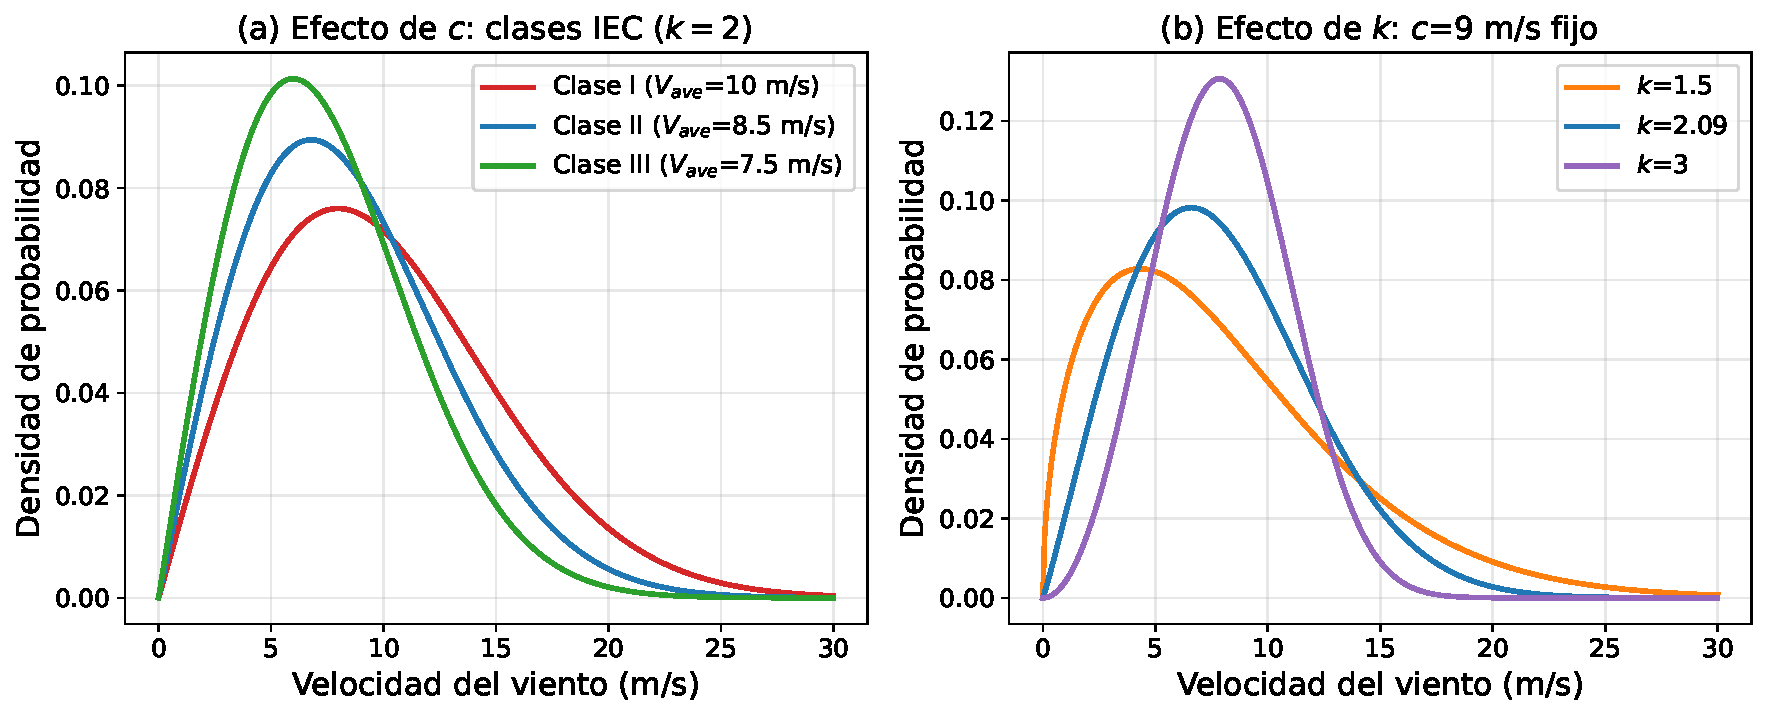
\includegraphics[width=\textwidth]{Figuras/Figuras Antecedentes/weibull_zonas.pdf}
    \caption{Efecto de los parámetros $c$ y $k$ de la distribución de Weibull.}
    \label{fig:weibull_zonas}
\end{figure}

\section{Marco normativo y condiciones de diseño}
\label{sec:marco-normativo}

La determinación de las cargas y la verificación estructural no dependen únicamente de modelos numéricos, sino también del cumplimiento de procedimientos establecidos por normas internacionales, que aseguran la integridad estructural ante condiciones ambientales extremas. El marco aplicable a este trabajo lo componen cuatro documentos de la serie IEC 61400, cada uno con un alcance distinto.

La norma IEC 61400-1 establece los requisitos generales de diseño y seguridad, y declara en su Sección 1 que se aplica a aerogeneradores de todos los tamaños, sin introducir restricción alguna respecto de la orientación del eje de rotación~\parencite{IEC61400-1}. La norma IEC 61400-3-1 extiende esos lineamientos al entorno marino de fundación fija y es la que prescribe las condiciones de viento sobre el mar que se emplean en este trabajo~\parencite{IEC61400-3-1}. La norma IEC 61400-3-2 aborda el caso de las estructuras flotantes, pertinente por la naturaleza del emplazamiento, si bien acota su alcance a plataformas no tripuladas con una única turbina de eje horizontal y advierte de forma expresa que las de eje vertical requieren consideraciones adicionales~\parencite{IEC61400-3-2}. Esa advertencia delimita con precisión el alcance de la presente verificación y se retoma al declarar sus limitaciones.

La norma IEC 61400-5, por último, es la específica de palas de aerogenerador y, por tanto, la directamente aplicable al objeto de este trabajo. Su Sección 1 declara que está destinada a las palas de todos los aerogeneradores y que la mayoría de los principios que recoge resultan aplicables a cualquier configuración de rotor, tamaño y material~\parencite{IEC61400-5}. Su pertinencia es doble, ya que además de los criterios de verificación estructural aporta un sistema de factores parciales de material más detallado que el de la IEC 61400-1 y una formulación de las cargas de pala que no presupone una geometría en voladizo, aspectos ambos que se desarrollan en las Secciones~\ref{sec:extrapolacion_teoria} y~\ref{sec:pandeo_teoria}.

\subsection{Parámetros de diseño y condiciones de carga}
\label{sec:condiciones_diseno}

Para garantizar la integridad estructural, la caracterización del viento según la norma IEC 61400-1 se organiza en el grupo de condiciones normales de operación, que definen el comportamiento recurrente del viento y los estados de carga de la estructura:

\textbf{Condiciones normales de viento (NWC, por sus siglas en inglés):} Incluyen el perfil de viento normal (NWP, por sus siglas en inglés), el cual describe la variación de la velocidad con la altura ($z$) mediante la ley de potencia de la Ec.~\ref{eq:nwp_ley_potencia}, con un exponente de cizalladura $\alpha_z$ que la norma IEC 61400-3-1 fija en $0{,}14$ para las condiciones normales de viento en emplazamientos marinos~\parencite{IEC61400-3-1}\glsunset{nwc}\glsunset{nwp}:

\begin{equation}
    V(z) = V_{hub} \left(\frac{z}{z_{hub}}\right)^{\alpha_z}
    \label{eq:nwp_ley_potencia}
\end{equation}

Asimismo, el modelo de turbulencia normal (NTM, por sus siglas en inglés)\glsunset{ntm} define la desviación estándar representativa de la turbulencia ($\sigma_{NTM}$) como el cuantil del $90\%$ de la desviación estándar de la velocidad para cada velocidad a la altura de referencia, y la expresa como una función lineal de esta última, según la Ec.~\ref{eq:ntm_sigma}:

\begin{equation}
    \sigma_{NTM} = I_{ref} \left(0{,}75 \, V_{hub} + b_{NTM}\right)
    \label{eq:ntm_sigma}
\end{equation}

donde $I_{ref}$ es la intensidad de turbulencia de referencia, parámetro adimensional que la norma tabula según la categoría de turbina ($0{,}16$ para la A, $0{,}14$ para la B y $0{,}12$ para la C) y que caracteriza la intensidad de las ráfagas esperada en el emplazamiento, y $b_{NTM}$ es el parámetro de ordenada de la recta, que la norma fija en $5{,}6$~m/s para las clases estándar~\parencite{IEC61400-1}.

Para el caso específico de las VAWT, todas las variables climáticas y de velocidad del viento se caracterizan a la altura del centro del área barrida por el rotor, notación que la norma denomina $z_{hub}$ por herencia de las \gls{hawt}, tal como se precisó en la Sección~\ref{sec:aerodinamica}.

\subsection{Modelo de turbulencia de Mann}
\label{sec:modelo_mann}

La norma IEC 61400-1 recomienda el modelo de cizalladura uniforme de Mann~\parencite{IEC61400-1,Mann1994} para la síntesis de turbulencia tridimensional. Se trata de un modelo \textit{espectral} porque no resuelve las ecuaciones de la dinámica de fluidos en el espacio físico, sino que define un tensor espectral de velocidades, esto es, una descripción de cómo se reparte la energía turbulenta entre remolinos de distinto tamaño y orientación, expresada en función del número de onda. El modelo parte del espectro isótropo de von Kármán y le aplica la distorsión que produce una cizalladura media uniforme, con lo que reproduce la anisotropía real de la turbulencia atmosférica: los remolinos no tienen la misma intensidad ni forma en todas las direcciones, sino que se elongan en la dirección del flujo~\parencite{IEC61400-1}.

El modelo queda determinado por tres parámetros que el Anexo C de la IEC 61400-1 fija a partir de las condiciones ya definidas para la clase de emplazamiento:

\begin{itemize}
    \item Un parámetro de \textbf{intensidad}, $\sigma_{iso}$, que establece el nivel de energía cinética turbulenta del campo generado y que la norma vincula a la desviación estándar representativa mediante $\sigma_{iso} = 0{,}55\,\sigma_{NTM}$. En la formulación original del modelo se expresa como $\alpha\varepsilon^{2/3}$, siendo $\varepsilon$ la tasa de disipación turbulenta~\parencite{Mann1994}.
    \item Una \textbf{escala de longitud}, $\ell = 0{,}8\,\Lambda_1$, que caracteriza el tamaño típico de los remolinos que concentran la mayor parte de la energía. Aquí $\Lambda_1$ es el parámetro de escala de turbulencia longitudinal definido en la Sección 6.3 de la norma, que para alturas menores a $60$~m vale $\Lambda_1 = 0{,}7\,z$. Una escala grande describe ráfagas que envuelven simultáneamente una porción extensa del rotor; una escala pequeña, fluctuaciones localizadas que afectan solo a un sector del área barrida.
    \item Un \textbf{parámetro de anisotropía}, $\Gamma$, que cuantifica cuánto deforma la cizalladura a los remolinos y que la norma fija en $\Gamma = 3{,}9$ por ajuste al modelo espectral de Kaimal.
\end{itemize}

A partir de estos tres parámetros, el algoritmo de simulación~\parencite{Mann1998} sintetiza una \textbf{caja de turbulencia} mediante transformada rápida de Fourier: una grilla tridimensional de puntos, con dos direcciones transversales al viento y una longitudinal que se traduce en tiempo al asumir que el campo turbulento es transportado por el flujo medio sin deformarse (hipótesis de turbulencia congelada de Taylor), en la que cada punto almacena las tres componentes de la velocidad fluctuante. QBlade los recibe como entrada bajo las denominaciones \textit{Alpha Epsilon}, \textit{L Mann} y \textit{Gamma}, y recorre la grilla resultante a medida que la turbina gira, alimentando el modelo aerodinámico con series temporales de viento tridimensional~\parencite{marten2019qblade}.

\subsection{Casos de carga de diseño}
\label{sec:dlc_seleccion}

Las condiciones de viento definidas anteriormente se combinan con los estados de operación de la turbina para formar los casos de carga de diseño (DLC, por sus siglas en inglés)\glsunset{dlc}, que la Tabla 2 de la IEC 61400-1 organiza en ocho situaciones de diseño: producción de potencia, producción con falla, arranque, parada normal, parada de emergencia, turbina estacionada, estacionada con falla, y transporte o mantenimiento~\parencite{IEC61400-1}.

Este trabajo se circunscribe a la primera de ellas, la producción de potencia, por corresponder al funcionamiento nominal de la turbina establecido en los objetivos. La delimitación se apoya en dos líneas de evidencia convergentes respecto del comportamiento de las palas de eje vertical. Por una parte, el análisis comparativo de \textcite{Galinos2015,Galinos2016} sobre un rotor Darrieus de $5$~MW muestra que, a diferencia de las \gls{hawt}, cuyo diseño suele quedar gobernado por la turbina estacionada bajo viento extremo, en una VAWT son las condiciones de operación normal con turbulencia las que producen las mayores cargas en la raíz de la pala y en la base de la torre. Por otra, la revisión histórica de \textcite{Sutherland2012} atribuye la falla prematura de buena parte de los primeros prototipos precisamente a haber subestimado las cargas dinámicas de origen turbulento durante la operación: se supuso que la turbulencia actuaba a frecuencias lo bastante bajas como para despreciarla, sin considerar que la sustentación que la pala genera al recorrer su trayectoria amplifica esas cargas y desplaza su contenido hacia frecuencias más altas, excitando los modos propios de la estructura.

La situación de producción de potencia comprende cinco casos de carga, que la norma agrupa según el tipo de fenómeno que representan~\parencite{IEC61400-1}:

\begin{itemize}
    \item \textbf{DLC 1.1 y 1.2:} recogen las cargas producidas por la turbulencia atmosférica que la turbina experimenta de forma habitual a lo largo de toda su vida, descrita mediante el \gls{ntm}. El primero se orienta a la resistencia última y el segundo a la fatiga.
    \item \textbf{DLC 1.3:} recoge las cargas últimas asociadas a condiciones de turbulencia excepcionalmente intensa, descritas mediante el modelo de turbulencia extrema (\gls{etm}, por sus siglas en inglés)\glsunset{etm}.
    \item \textbf{DLC 1.4 y 1.5:} corresponden a eventos transitorios concretos, seleccionados por la norma como potencialmente críticos: una ráfaga coherente extrema acompañada de un cambio de dirección (\gls{ecd}, por sus siglas en inglés)\glsunset{ecd} y una cizalladura de viento extrema (\gls{ews}, por sus siglas en inglés)\glsunset{ews}, respectivamente.
\end{itemize}

La diferencia entre ambos grupos está en la naturaleza del viento que los define. Los casos 1.1 a 1.3 son \textbf{estocásticos}: el viento se describe como un proceso aleatorio, del que no se conoce el valor instantáneo pero sí sus propiedades estadísticas (media, desviación estándar y contenido espectral), por lo que cada caso debe simularse varias veces con distintas semillas aleatorias y la carga de diseño se obtiene por tratamiento estadístico del conjunto de resultados. Los casos 1.4 y 1.5, en cambio, son \textbf{determinísticos}: la norma define para ellos una forma temporal de ráfaga o de cizalladura fija y reproducible, de modo que basta una simulación por condición y la carga de diseño es el valor máximo alcanzado durante el transitorio.

Conviene matizar la delimitación al régimen de producción de potencia a la luz de literatura más reciente. \textcite{Moore2024} observan que los estudios previos sobre casos de carga críticos en VAWT se concentraron en rotores Darrieus de gran tamaño y elevada flexibilidad, y que al reevaluar los DLC sobre un H-rotor pequeño y rígido aparecen tasas de daño por fatiga no despreciables en casos habitualmente descartados, como la turbina estacionada, la cizalladura extrema y la ráfaga con cambio de dirección; \textcite{Sakib2022}, por su parte, advierten que en VAWT flotantes la condición estacionada es una preocupación de primer orden, dado que la ausencia de control de paso mantiene el rotor cargado durante todo el temporal. Ambos trabajos abordan, sin embargo, aspectos distintos del problema tratado aquí (turbinas de escala reducida, cubiertas por la IEC 61400-2, y el dimensionamiento de la plataforma y del fondeo antes que de la pala), pero delimitan con precisión el alcance de esta memoria: la verificación desarrollada corresponde al régimen de producción de potencia y no permite descartar, por sí sola, que otros casos resulten dimensionantes, aspecto que se retoma entre las proyecciones del trabajo.

\subsection{Extrapolación estadística de cargas extremas}
\label{sec:extrapolacion_teoria}

Para determinar la carga característica del DLC 1.1 a partir de simulaciones con flujo turbulento, la norma remite a su Anexo G, de carácter informativo~\parencite{IEC61400-1}. El problema que este anexo resuelve es directo: la pala falla si la tensión en algún punto supera la resistencia del material, de modo que verificarla exige conocer la mayor carga que experimentará en su vida útil. Esa carga no puede medirse ni simularse directamente, ya que simular veinte años de operación es inviable y en la práctica solo se dispone de unas pocas realizaciones de diez minutos, cuyo máximo observado es casi con certeza menor que el que llegará a ocurrir en dos décadas. La pregunta relevante no es entonces cuál fue el máximo simulado, sino qué tan grande puede ser uno que todavía no se ha observado, interrogante que el Anexo G responde mediante teoría de valores extremos~\parencite{IEC61400-1}.

La norma precisa además sobre qué magnitudes debe operar ese análisis. Su Sección 7.4.2 establece que el tratamiento estadístico de los datos del DLC 1.1 debe incluir, como mínimo, el cálculo de los valores extremos del momento en la raíz de la pala en el plano y fuera del plano, y de la deflexión de punta~\parencite{IEC61400-1}. Esa formulación constituye la abreviatura válida para una pala en voladizo desde el buje, geometría en la que el momento en la raíz es por construcción el máximo a lo largo de la envergadura y basta por tanto para caracterizar la solicitación.

La norma específica de palas adopta una formulación general que no presupone esa geometría, apoyada en el concepto de envolvente de cargas, que su Sección 3.17 define como el conjunto de cargas de diseño máximas en todas las direcciones y en todas las posiciones a lo largo de la envergadura~\parencite{IEC61400-5}. Dicha definición resulta igualmente aplicable a un voladizo y a una viga sostenida en dos apoyos, configuración esta última que corresponde a la pala de un H-rotor descrita en la Sección~\ref{sec:analisis-estructural}, y en la que existen tres secciones candidatas a gobernar en lugar de una. La correspondencia entre ambas formulaciones es directa, puesto que la Sección 3.1 de esa misma norma identifica la raíz con la parte de la pala que se conecta a la estructura del rotor~\parencite{IEC61400-5}, que en un H-rotor son sus conexiones con los brazos de soporte.

Respecto de las direcciones sobre las que debe construirse esa envolvente, la Sección 6.1.4.3 distingue un enfoque básico, que emplea cuatro conjuntos de cargas correspondientes a los extremos en el plano y fuera del plano, de un enfoque avanzado que considera todas las direcciones potencialmente críticas dentro de una sección y para el que la norma considera suficiente, a falta de un análisis específico de criticidad, un conjunto de cargas distribuido uniformemente en al menos doce direcciones~\parencite{IEC61400-5}. La elección entre ambos no es indiferente, ya que condiciona directamente uno de los factores parciales de material que se describen en la Sección~\ref{sec:comportamiento_laminado}.

El razonamiento se apoya en dos ideas. La primera es que, para una velocidad de viento dada, la carga sobre la pala puede tratarse como un proceso aleatorio estacionario: sus propiedades estadísticas no cambian mientras esa condición de viento se mantenga. La segunda es que los máximos de ese proceso ocurren suficientemente separados en el tiempo como para considerarlos estadísticamente independientes entre sí. Bajo esos supuestos, el comportamiento del máximo de un conjunto grande de observaciones deja de depender del detalle del proceso y converge hacia una familia acotada de distribuciones, resultado clásico de la teoría de valores extremos~\parencite{Gumbel1958}. Entre ellas, la distribución de Gumbel describe los máximos provenientes de procesos con cola de tipo exponencial y queda definida por la Ec.~\ref{eq:gumbel_anexof}:

\begin{equation}
\Phi(F; \mu_j, \beta_j) = \exp\left[ -\exp\left( -\frac{F - \mu_j}{\beta_j} \right) \right]
\label{eq:gumbel_anexof}
\end{equation}

donde $\Phi$ es la probabilidad acumulada de que el máximo de una realización de diez minutos no supere el nivel de carga $F$ (N o N$\cdot$m, según la componente que se analice); $F$ es el nivel de carga evaluado; $\mu_j$ es el parámetro de posición, que sitúa la distribución ajustada a la velocidad $V_j$ e indica el orden de magnitud de los máximos a esa velocidad; y $\beta_j$ es el parámetro de escala, que mide su dispersión, esto es, cuánto varían los máximos entre una realización y otra. Ambos parámetros se estiman a partir de los máximos observados mediante el método de los momentos, que iguala la media y la varianza de la distribución a las de la muestra~\parencite{Gumbel1958}. Lo relevante del ajuste no es reproducir los datos ya observados, sino describir la \textit{cola} de la distribución, la zona de cargas altas y poco frecuentes donde no hay observaciones y que es la que interesa extrapolar. La probabilidad de excedencia condicionada a una velocidad, Ec.~\ref{eq:pe_cond_anexof}, se lee entonces como la fracción de realizaciones de diez minutos a esa velocidad en que la carga superaría el nivel $F$:

\begin{equation}
P_e(F \mid V_j) = 1 - \Phi(F; \mu_j, \beta_j)
\label{eq:pe_cond_anexof}
\end{equation}

La turbina, sin embargo, no opera siempre a la misma velocidad, y una carga muy alta puede ser probable a $24$~m/s y a la vez irrelevante si el emplazamiento casi nunca alcanza esa velocidad. El riesgo no se evalúa por eso velocidad por velocidad, sino ponderando cada una por el tiempo que el viento efectivamente permanece en ella, información que aporta la distribución de Weibull del sitio, $f_W(V)$. Esa ponderación es la integral de la Ec.~\ref{eq:pe_longterm_anexof}, que combina la severidad de cada condición con su frecuencia de ocurrencia:

\begin{equation}
P_e(F) = \int_{V_{in}}^{V_{out}} P_e(F \mid V) \cdot f_W(V) \, dV
\label{eq:pe_longterm_anexof}
\end{equation}

donde $P_e(F)$ es la probabilidad de excedencia de largo plazo del nivel de carga $F$, es decir, considerando todo el rango de operación; $P_e(F \mid V)$ es la probabilidad de excedencia condicionada a la velocidad $V$, dada por la Ec.~\ref{eq:pe_cond_anexof}; $f_W(V)$ es la función de densidad de probabilidad de la velocidad del viento en el emplazamiento, obtenida del ajuste de Weibull de la Ec.~\ref{eq:weibull_cdf}; y $V_{in}$ y $V_{out}$ son las velocidades de conexión y de desconexión de la turbina, que acotan el rango en que la máquina se encuentra produciendo potencia.

Queda por definir qué probabilidad resulta aceptable. Si la carga característica debe ser excedida, en promedio, una sola vez cada $T_{retorno}$, y cada realización representa un intervalo de duración $T_{obs}$, la probabilidad admisible por realización es el recíproco del número de intervalos que caben en el período de retorno, según la Ec.~\ref{eq:fk_anexof}:

\begin{equation}
P_e(F_k) = \frac{T_{obs}}{T_{retorno}}
\label{eq:fk_anexof}
\end{equation}

donde $P_e(F_k)$ es la probabilidad de excedencia admisible por realización; $T_{obs}$ es la duración de cada realización simulada, en este caso los diez minutos que la norma establece como ventana de referencia; y $T_{retorno}$ es el período de retorno, entendido como el intervalo medio de tiempo que transcurre entre dos ocurrencias sucesivas de un evento de esa magnitud, que para el DLC 1.1 la norma fija en $50$ años en su Sección 7.6.2~\parencite{IEC61400-1}. Decir que una carga tiene un período de retorno de $50$ años no significa que se presente exactamente una vez cada cincuenta años, sino que, en promedio y a lo largo de un plazo suficientemente extenso, se espera que sea superada una vez en ese lapso; equivale, por tanto, a asignarle una probabilidad anual de excedencia de $1/50$.

Para el período de retorno de $50$ años y realizaciones de diez minutos, esta razón vale $3{,}8 \times 10^{-7}$, valor que la propia norma señala en esa sección como la probabilidad de excedencia máxima admisible, y cuya magnitud explica por qué el procedimiento es indispensable: se busca un nivel de carga con una probabilidad de ocurrencia del orden de una en varios millones, que ninguna cantidad razonable de simulaciones podría observar de forma directa. La carga característica $F_k$ es el valor que satisface esa igualdad, y se obtiene invirtiendo numéricamente la Ec.~\ref{eq:pe_longterm_anexof}.

Finalmente, $F_k$ es una estimación estadística y arrastra las incertidumbres del modelo aerodinámico, del número finito de realizaciones y del ajuste de la cola. La norma cubre ese margen mayorando la carga mediante un factor parcial de seguridad, según la Ec.~\ref{eq:fd_anexof}:

\begin{equation}
F_d = \gamma_f \cdot F_k
\label{eq:fd_anexof}
\end{equation}

donde $F_d$ es la carga de diseño con que se verifica la estructura, $F_k$ la carga característica obtenida de la extrapolación y $\gamma_f$ el factor parcial de seguridad aplicado a la carga. Para el DLC 1.1 la Tabla 3 asigna $\gamma_f = 1{,}25$, menor que el $1{,}35$ general, porque al haberse realizado ya una extrapolación estadística explícita hasta los 50 años, parte del conservadurismo que el factor general debe cubrir está incorporado en la propia carga característica.

El desarrollo completo del procedimiento, incluidos los criterios de verificación del ajuste de la distribución y los métodos alternativos de agregación de máximos, se encuentra en el Anexo G de la IEC 61400-1~\parencite{IEC61400-1}.

\subsection{Evaluación del daño acumulado por fatiga}
\label{sec:anexo_g_antecedentes}

La verificación anterior responde a si la pala resiste la carga más severa de su vida. La fatiga plantea una pregunta distinta y, para una pala de VAWT, más exigente: si sobrevive la repetición de cargas que individualmente no la dañarían. Como se describió en la Sección~\ref{sec:dynamicstall}, cada revolución del rotor somete a la pala a un ciclo completo de carga, de modo que en veinte años se acumulan del orden de $10^9$ ciclos. El daño no proviene entonces de un evento extremo, sino de la suma de millones de solicitaciones moderadas.

Para el DLC 1.2 la norma remite igualmente a un anexo informativo, el Anexo H~\parencite{IEC61400-1}, que organiza el cálculo en cuatro pasos, cada uno de los cuales responde a una necesidad concreta. La Figura~\ref{fig:rainflow_sn} los ilustra sobre un segmento de serie temporal a una sola velocidad de viento, unidad básica del procedimiento.

El primero es identificar los ciclos. Una serie temporal de carga real no es una sinusoide limpia sino una señal irregular, con oscilaciones grandes interrumpidas por otras pequeñas, y no resulta evidente qué máximo debe emparejarse con qué mínimo para constituir un ciclo. La respuesta tiene fundamento físico: el daño se asocia a cada lazo de histéresis cerrado en el diagrama tensión-deformación del material, de modo que el emparejamiento correcto es el que reconstruye esos lazos, y eso es exactamente lo que hace el algoritmo de conteo Rainflow, devolviendo un conjunto de ciclos caracterizados por su amplitud $S_a$ y su tensión media $S_m$, según se representa en el panel (a) de la Figura~\ref{fig:rainflow_sn}. El método fue propuesto por \textcite{Matsuishi1968}, quienes lo describieron por analogía con el agua de lluvia escurriendo sobre un tejado de pagoda, de donde toma su nombre; su formulación algorítmica normalizada corresponde a la práctica ASTM E1049-85~\parencite{ASTM_E1049}.

El segundo paso es referir todos los ciclos a una condición común. La curva S-N de un material se obtiene de ensayos de amplitud constante realizados a una razón de tensiones fija, de modo que describe directamente solo los ciclos cuya tensión media coincide con la del ensayo. Los ciclos reales ocurren, en cambio, sobre niveles medios diversos, y ese nivel no es un detalle secundario: una misma amplitud resulta tanto más dañina cuanto mayor es la tensión media sobre la que se superpone, porque la tensión máxima del ciclo se aproxima más a la resistencia del material. El caso es particularmente relevante en una \gls{vawt}, donde la fuerza centrífuga impone una tracción permanente sobre la que se superponen las fluctuaciones aerodinámicas. Por esa razón la Sección 7.6.3.1 de la norma exige que el cálculo de daño considere tanto el rango cíclico como el nivel de tensión media~\parencite{IEC61400-1}.

El instrumento habitual para incorporar ese efecto es el diagrama de vida constante, que convierte cada par $(S_a, S_m)$ en la amplitud equivalente a tensión media nula que produce el mismo daño, con lo que la curva S-N vuelve a ser aplicable. Su forma lineal es la de Goodman, Ec.~\ref{eq:goodman}:

\begin{equation}
S_{a,0} = \frac{S_a}{1 - \dfrac{S_m}{S_u}}
\label{eq:goodman}
\end{equation}

donde $S_{a,0}$ es la amplitud equivalente, $S_m$ la tensión media del ciclo y $S_u$ la resistencia última a tracción del material. La alternativa parabólica de Gerber sustituye ese cociente por su cuadrado y entrega, para una misma tensión media, una amplitud equivalente menor, por lo que resulta menos conservadora que la de Goodman.

El tercer paso es traducir cada ciclo en daño. Para ello se recurre a la curva S-N del material (del inglés \textit{stress-number of cycles}, tensión frente a número de ciclos, también llamada curva de Wöhler), que relaciona la amplitud de tensión aplicada con el número de ciclos que el material soporta antes de fallar bajo esa amplitud constante. Para compuestos y metales en régimen de alto número de ciclos, esta relación se describe adecuadamente mediante la ley potencial de Basquin, Ec.~\ref{eq:sn_basquin}:

\begin{equation}
S = S_f' \, (2N_f)^b
\label{eq:sn_basquin}
\end{equation}

donde $S$ es la amplitud de tensión aplicada, que tras la corrección del paso anterior corresponde a $S_{a,0}$; $N_f$ es el número de ciclos que el material soporta bajo esa amplitud constante antes de fallar, de modo que $2N_f$ representa el número de inversiones de carga, ya que cada ciclo contiene dos; $S_f'$ es el coeficiente de resistencia a fatiga, que fija la posición de la recta en el diagrama doblemente logarítmico y equivale a la tensión que provocaría la falla en una única inversión; y $b$ es el exponente de Basquin, que fija su pendiente. Tanto $S_f'$ como $b$ son propiedades del material obtenidas experimentalmente; en la práctica habitual para compuestos, y también en este trabajo, $S_f'$ se identifica con la resistencia última a tracción $\sigma_u$, lo que equivale a hacer pasar la recta por el punto correspondiente a la falla en una inversión. El exponente $b$ es negativo y de valor pequeño, de modo que una reducción modesta en la amplitud de tensión se traduce en un aumento de varios órdenes de magnitud en la vida admisible, y unos pocos ciclos de gran amplitud pueden dominar el daño total por encima de millones de ciclos pequeños.

El cuarto paso es sumar. La hipótesis de Palmgren-Miner supone que cada ciclo consume una fracción de la vida del material igual a $1/N_i$, y que esas fracciones se acumulan de forma lineal e independiente del orden en que ocurren~\parencite{Miner1945}, lo que conduce a la Ec.~\ref{eq:miner_anexog}:

\begin{equation}
D = \sum_i \frac{n_i}{N_i}
\label{eq:miner_anexog}
\end{equation}

donde $D$ es el daño acumulado, magnitud adimensional que expresa la fracción de vida consumida; $n_i$ es el número de ciclos efectivamente aplicados con amplitud correspondiente al rango $i$, dato que entrega el conteo Rainflow; y $N_i$ es el número de ciclos admisibles para esa misma amplitud, dato que entrega la curva S-N mediante la Ec.~\ref{eq:sn_basquin}. La independencia del orden es una simplificación, ya que en la realidad la secuencia de cargas influye en la propagación del daño, pero es la hipótesis que la norma adopta por su robustez y simplicidad. La condición de verificación es $D \leq 1$, valor que no debe interpretarse como el instante exacto de la rotura: dado que la curva S-N de diseño se construye con una probabilidad de supervivencia elevada, $D = 1$ señala el punto en que se agota el nivel de confiabilidad buscado, no la falla física garantizada.

\begin{figure}[H]
    \centering
    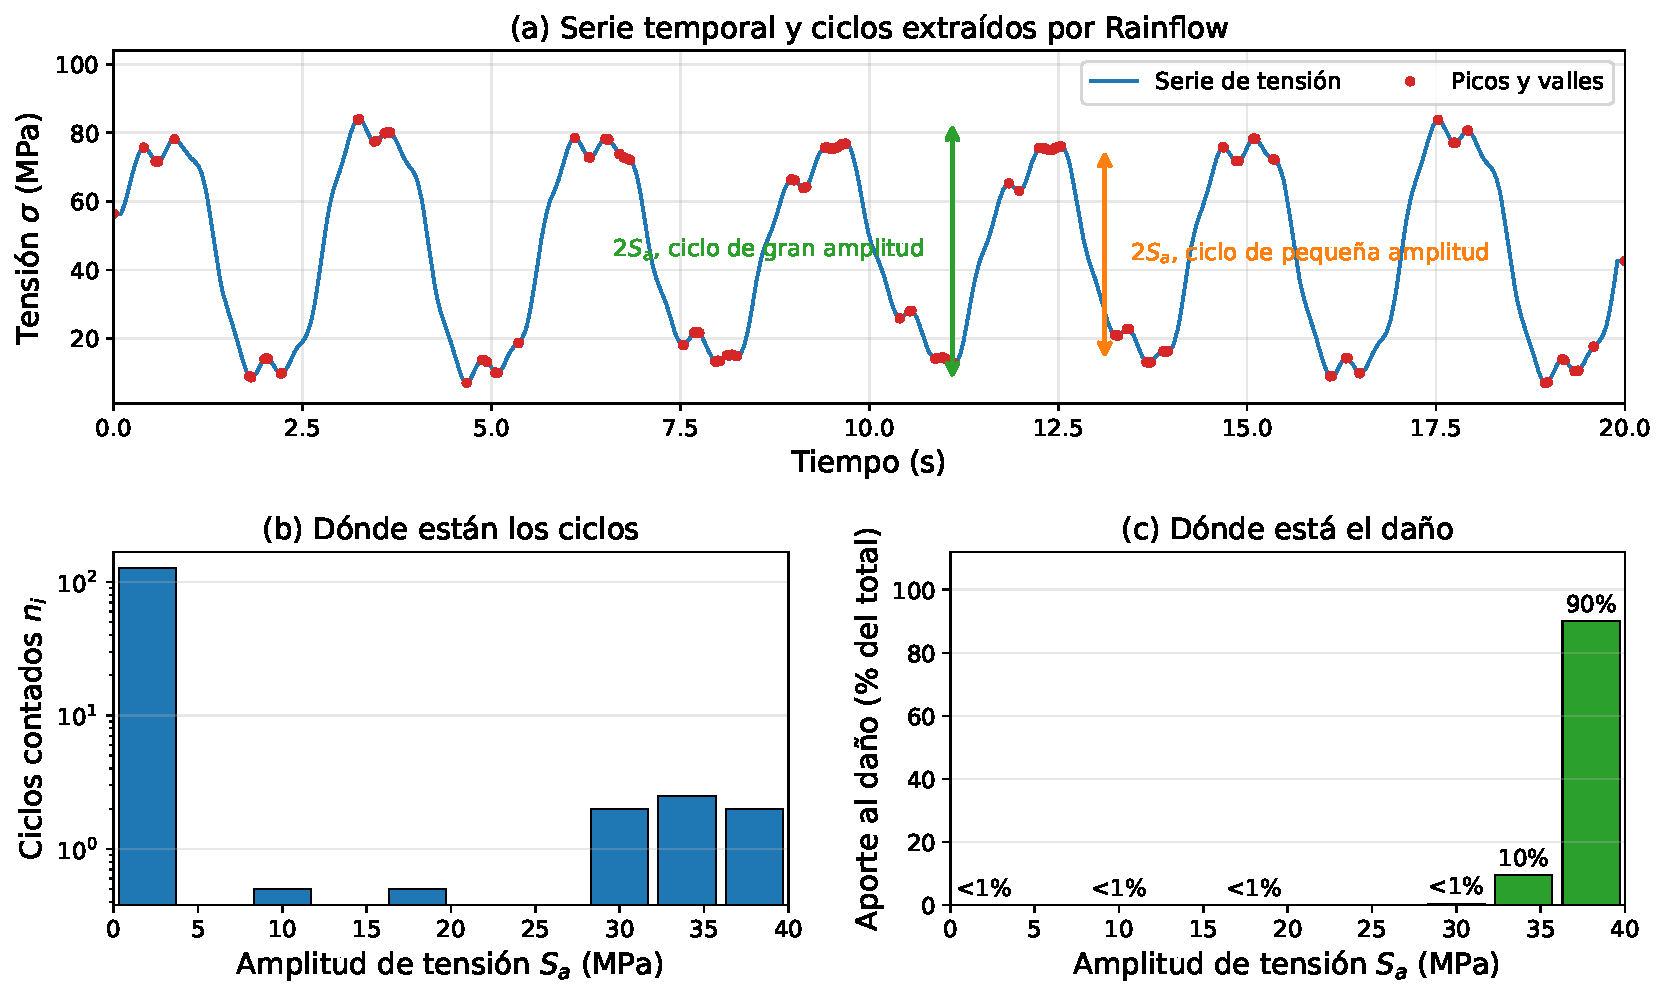
\includegraphics[width=\textwidth]{Figuras/Figuras Antecedentes/rainflow_sn.pdf}
    \caption[Procedimiento de fatiga del Anexo H de la IEC 61400-1.]{Procedimiento de fatiga del Anexo H de la IEC 61400-1 sobre un segmento ilustrativo de serie temporal: (a) ciclos identificados por el conteo Rainflow, (b) espectro de ciclos resultante y (c) aporte de cada rango al daño, evaluado con la curva S-N factoreada (Ec.~\ref{eq:sn_basquin}) para el GFRP empleado en este trabajo.}
    \label{fig:rainflow_sn}
\end{figure}

\newpage
Los paneles (b) y (c) de la Figura~\ref{fig:rainflow_sn} muestran ese efecto sobre el segmento simulado: los dos ciclos de mayor amplitud, asociados a la revolución completa del rotor, concentran el $90\%$ del daño, mientras que los $132$ restantes, de origen turbulento, aportan el resto. De ahí que la verificación de fatiga sea sensible sobre todo a la correcta reproducción de las oscilaciones de gran amplitud.

Resta un aspecto propio de la aplicación a aerogeneradores. Las series simuladas duran minutos y cada una corresponde a una única velocidad de viento, mientras que el daño debe evaluarse sobre veinte años de operación a velocidades que varían continuamente. El objeto que salva esa distancia es el \textit{espectro de carga representativo}: un único recuento de ciclos que resume cuántas veces, y con qué amplitud, se solicita la pala a lo largo de un año típico de operación en el emplazamiento.

Su construcción encadena tres operaciones. La primera es aplicar el conteo Rainflow por separado a la serie de cada velocidad de viento simulada, lo que entrega un espectro parcial, esto es, el número de ciclos $n_i$ por rango de amplitud $S_a$ que la pala experimenta durante los minutos simulados a esa velocidad. La segunda es llevar cada espectro parcial a la escala de un año, multiplicándolo por la razón entre la duración del año y la de la simulación, y por la fracción del año en que el viento permanece en el intervalo de velocidad correspondiente, dato que entrega la distribución de Weibull del emplazamiento (Sección~\ref{sec:recurso_eolico}): así, dos condiciones de viento simuladas durante el mismo tiempo no contribuyen igual al daño anual si una ocurre la mitad del año y la otra apenas unas horas. La tercera operación es sumar los espectros parciales así escalados, rango a rango, con lo que se obtiene el espectro anual. La aplicación numérica de este procedimiento al caso de estudio se desarrolla en la Sección~\ref{sec:anexo_g}.

Con ese espectro, la aplicación de la regla de Miner es inmediata: cada rango de amplitud aporta $n_i/N_i$, donde $N_i$ se lee sobre la curva S-N factoreada, y el daño anual es la suma de esos aportes; multiplicado por la vida de diseño se obtiene el daño acumulado que debe compararse con la unidad.

La vida útil de diseño adoptada para el cálculo es de $20$ años, período que la Sección 6.2 de la IEC 61400-1 establece como vida de diseño mínima para las turbinas de las clases I a III y que constituye, por tanto, el horizonte de referencia frente al cual la norma exige demostrar que $D \leq 1$~\parencite{IEC61400-1}.

Por último, la curva S-N se emplea en su forma factoreada, reduciendo la resistencia mediante el factor parcial de material $\gamma_m = 1{,}7$, valor que la norma asigna a los materiales compuestos con coeficiente de variación de la resistencia entre el $15\%$ y el $20\%$ (Sección 7.6.3.2). El factor parcial aplicado a la carga es, en cambio, $\gamma_f = 1{,}0$ (Sección 7.6.3.1): a diferencia del estado límite último, en fatiga la norma concentra el margen de seguridad en el lado de la resistencia y no en el de la solicitación, por cuanto la incertidumbre dominante proviene de la dispersión de las propiedades del material antes que de la magnitud de las cargas. La curva S-N correspondiente al material empleado en este trabajo, en sus formas nominal y factoreada, se presenta en la Figura~\ref{fig:curva_sn_gfrp}.

\section{Herramientas de simulación aerodinámica}
\label{sec:herramientas}

Una vez definidos el recurso eólico y las condiciones de diseño establecidas por la IEC 61400, resulta necesario emplear herramientas numéricas capaces de reproducir el comportamiento aerodinámico y estructural de la turbina bajo dichas condiciones. Esta sección presenta primero el panorama de los principales métodos disponibles, ordenados de menor a mayor fidelidad, y a continuación el programa QBlade y los submodelos que incorpora, por ser la herramienta sobre la que se apoya el desarrollo posterior. La selección del método y su configuración corresponden a decisiones metodológicas y se justifican en el Capítulo~3.

Esa simulación representa un desafío computacional considerable por la naturaleza inestable de la aerodinámica de las \gls{vawt}: a diferencia de las \gls{hawt}, donde el flujo se aproxima de manera axial y el ángulo de ataque permanece relativamente constante, las palas de un H-rotor experimentan variaciones extremas y cíclicas del ángulo de ataque y atraviesan continuamente su propia estela turbulenta, cinemática que exige resolver fenómenos no lineales como el desprendimiento dinámico de la capa límite y la interacción pala-estela.

\subsection{Métodos aerodinámicos}
\label{sec:metodos_aerodinamicos}

Históricamente, la evaluación aerodinámica de las \gls{vawt} se ha fundamentado en modelos basados en la teoría del momento, siendo el modelo de tubo de corriente múltiple doble (DMST, por sus siglas en inglés)\glsunset{dmst} el más extendido en la ingeniería clásica. Propuesto originalmente por \textcite{Paraschivoiu2002}, el método \gls{dmst} discretiza el rotor en un conjunto de tubos de corriente bidimensionales independientes y divide cada tubo en dos actuadores sucesivos: uno en el semiciclo de barlovento (\textit{upwind}) y otro en el de sotavento (\textit{downwind}). Ambos semiciclos corresponden a las dos mitades del recorrido acimutal identificadas en la Figura~\ref{fig:top_view}: en el de barlovento la pala enfrenta el flujo todavía no perturbado por el rotor, mientras que en el de sotavento lo hace después de que ese mismo flujo ha atravesado la mitad anterior y ha cedido parte de su energía, de modo que llega con velocidad reducida.

Aunque este enfoque permite una estimación algorítmicamente rápida del coeficiente de potencia ($C_p$) y se emplea habitualmente en etapas tempranas de diseño, presenta limitaciones físicas severas: no captura la expansión tridimensional de la estela y pierde precisión de forma drástica en regímenes de alta relación de velocidad de punta ($\lambda$), donde los efectos del flujo inestable dominan el comportamiento del rotor~\parencite{Galinos2015,Tchakoua2015}. Ese umbral no está fijado universalmente, pues la degradación depende también de la solidez del rotor, pero las fuentes lo sitúan hacia el extremo superior del rango en que estas máquinas efectivamente operan: $\lambda = 2$ a $5$ para una configuración H-Darrieus óptima (Tabla~\ref{tab:tabla_vawt}), próximo al \gls{tsr} objetivo de $3{,}8$ de la T1-turbine, de escala comparable a la del caso de estudio (Tabla~\ref{tab:t1_params}). Por su naturaleza cuasi-estática, el DMST sobrestima sistemáticamente el coeficiente de potencia, con valores de $C_p$ que pueden superar $0{,}50$ para configuraciones H-Darrieus, muy por encima del rango validado experimentalmente ($0{,}35\text{--}0{,}45$)~\parencite{Essahraoui2026}. La revisión de \textcite{Islam2008} sobre modelos aerodinámicos para rotores Darrieus de pala recta confirma que el \gls{dmst} no resulta adecuado ni a TSR elevados ni en rotores de alta solidez, mientras que los modelos de vórtices, aun siendo los más precisos, son computacionalmente costosos y pueden presentar problemas de convergencia. Con todo, el bajo costo del \gls{dmst} lo mantiene entre los modelos más extendidos para la estimación preliminar~\parencite{Islam2008}, y es la razón por la que QBlade lo incorpora junto al método de vórtices libres~\parencite{marten2019qblade}.

Para superar estas deficiencias sin incurrir en el costo de las simulaciones viscosas tridimensionales por dinámica de fluidos computacional (CFD, por sus siglas en inglés)\glsunset{cfd}, el estado del arte ha convergido hacia los métodos basados en la teoría de vórtices, entre los cuales el de línea sustentadora con estela de vórtice libre (LLFVW, por sus siglas en inglés)\glsunset{llfvw} se posiciona como una de las herramientas de mayor fidelidad para el análisis aerodinámico de rotores complejos~\parencite{Galinos2015,marten2019qblade}.

Bajo la formulación \gls{llfvw}, las palas del aerogenerador se modelan como líneas de sustentación discretizadas que emiten continuamente filamentos de vorticidad hacia el fluido, según el esquema de la Figura~\ref{fig:llfvw_esquema}. La pala se divide en paneles y se sustituye por una línea situada a un cuarto de cuerda, sobre la que se distribuyen vórtices ligados cuya intensidad reproduce la sustentación local, determinada a partir de la velocidad relativa y de los coeficientes tabulados del perfil~\parencite{marten2019qblade}. De los bordes de cada panel se desprenden dos tipos de filamentos: los vórtices de arrastre (\textit{trailing vortices}), que se extienden aguas abajo y se originan en la variación espacial de la sustentación a lo largo de la envergadura, y los vórtices de desprendimiento (\textit{shed vortices}), que unen transversalmente a los anteriores y se generan en cada paso de tiempo por la variación temporal de la circulación propia del flujo cíclico. El conjunto forma una malla de vorticidad que se convecta, deforma e interactúa libremente en el espacio, sin que su geometría se imponga de antemano, bajo la influencia de sus propias velocidades inducidas. El cálculo de esas velocidades se vuelve singular cuando el punto evaluado cae sobre el propio filamento, por lo que los códigos asignan a cada vórtice un radio de núcleo dentro del cual la velocidad inducida decae suavemente a cero, con lo que se evita la inestabilidad numérica y se representa a la vez el núcleo viscoso real del vórtice~\parencite{marten2019qblade}.

\begin{figure}[H]
    \centering
    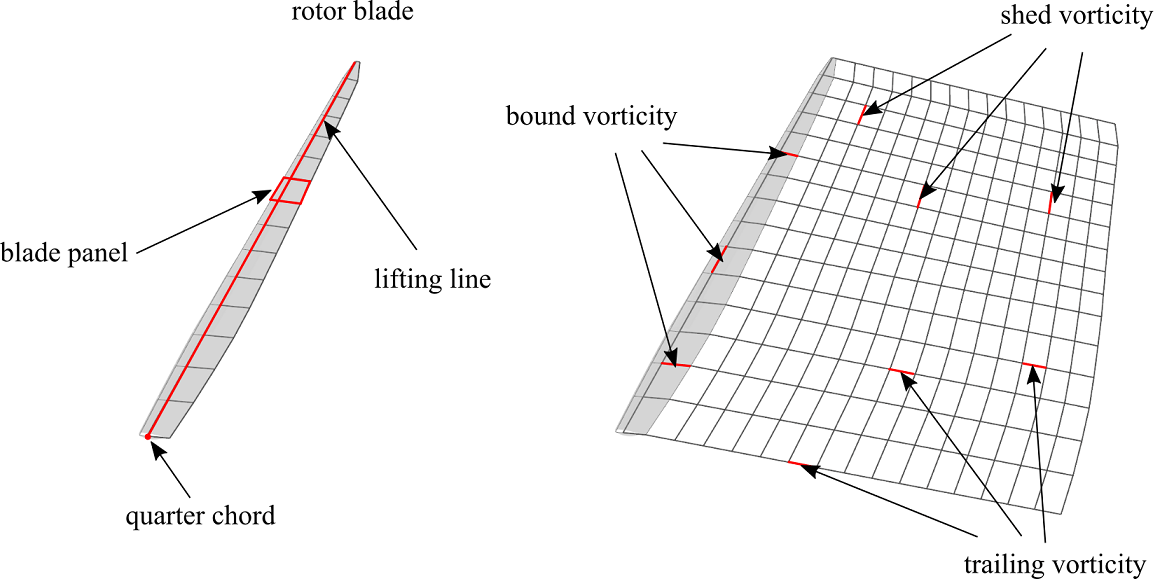
\includegraphics[width=0.7\textwidth]{Figuras/Figuras Antecedentes/qblade_llfvw_bladewake.png}
    \caption[Elementos del modelo de pala y de estela del algoritmo LLFVW.]{Elementos del modelo de pala y de estela del algoritmo LLFVW: panelado de la pala y línea sustentadora a un cuarto de cuerda (izquierda), y vorticidad ligada, de desprendimiento (\textit{shed}) y de arrastre (\textit{trailing}) sobre la malla de estela (derecha). Tomado de la documentación oficial~\parencite{QBladeDocs2024}.}
    \label{fig:llfvw_esquema}
\end{figure}

Resolver la estela de este modo, en lugar de prescribir su geometría, es lo que vuelve al método apropiado para un H-rotor. Como se expuso en la Sección~\ref{sec:aerodinamica}, la pala recorre el semiciclo de sotavento atravesando la estela que ella misma y las restantes palas generaron al pasar por barlovento, fenómeno que \textcite{Ferreira2009} registraron experimentalmente mediante \gls{piv}. La posición de ese encuentro depende de cuánto se ha convectado y deformado la estela en el intervalo transcurrido, de manera que un modelo de estela prescrita no puede reproducirlo. Al calcular esa evolución de forma explícita, el algoritmo \gls{llfvw} entrega la fluctuación de carga asociada al cruce, junto con las pérdidas de punta de pala y el efecto del flujo transversal sobre la estructura~\parencite{Galinos2015,marten2019qblade}: esa fluctuación constituye el ciclo de carga que gobierna la fatiga de la pala y es, por tanto, la magnitud que interesa en este trabajo.

La circulación ligada no se conoce de antemano. La fuerza sobre cada panel depende de la velocidad relativa que este percibe, y esa velocidad incluye la inducción de todos los vórtices del sistema, cuya intensidad es a su vez la incógnita que se busca. El método resuelve esa dependencia mutua de forma iterativa dentro de cada paso temporal: mantiene congelada la geometría de la estela, evalúa una sola vez las velocidades que esta induce sobre los paneles del rotor, y actualiza la circulación ligada hasta que su valor deja de cambiar dentro de una tolerancia prescrita, momento en que las fuerzas del paso quedan determinadas~\parencite{marten2019qblade}. Este lazo se conoce como iteración de circulación, o iteración Gamma por el símbolo $\Gamma$ con que la magnitud se denota, y tanto su tolerancia como el número máximo de iteraciones admitidas constituyen parámetros de configuración del cálculo.

Las familias de métodos descritas no compiten entre sí, sino que ocupan posiciones distintas en lo que \textcite{Essahraoui2026} denominan una jerarquía de fidelidad física, costo computacional y alcance predictivo creciente. La Tabla~\ref{tab:comparacion_metodos} las resume ordenadas de menor a mayor fidelidad, a partir de la revisión de modelos aerodinámicos para rotores Darrieus de pala recta de \textcite{Islam2008} y de la revisión crítica de \textcite{Essahraoui2026}, que actualiza la comparación incorporando los métodos de \gls{cfd}.

\begin{table}[H]
    \centering
    \caption{Comparación de los métodos aerodinámicos para VAWT, ordenados de menor a mayor fidelidad. Elaborada a partir de las revisiones de \textcite{Islam2008} y \textcite{Essahraoui2026}.}
    \label{tab:comparacion_metodos}
    \renewcommand{\arraystretch}{1.2}
    \footnotesize
    \begin{tabular}{p{2.2cm} p{3.3cm} p{3.4cm} p{4.4cm}}
        \hline
        \textbf{Método} & \textbf{Principio} & \textbf{Ventajas} & \textbf{Limitaciones} \\
        \hline
        Momento (DMST) &
        Balance de cantidad de movimiento en tubos de corriente, con factores de inducción independientes para los semiciclos de barlovento y sotavento &
        Costo mínimo; adecuado para barridos paramétricos y estimación preliminar del TSR; captura la asimetría barlovento-sotavento &
        Cuasi-estático: emplea polares estáticas y desatiende la pérdida dinámica y la curvatura de flujo; sobrestima la potencia en rotores de alta solidez y presenta problemas de convergencia a TSR elevados~\parencite{Islam2008,Essahraoui2026} \\
        Vórtices libres (LLFVW) &
        Palas modeladas como líneas sustentadoras que emiten filamentos de vorticidad que convectan libremente en el dominio &
        Resuelve la sustentación inestable, la geometría de la estela y la interacción pala-estela; costo órdenes de magnitud inferior al del CFD resuelto en la pala, compatible con series temporales largas &
        Considerado el más preciso de los modelos clásicos, pero mucho más costoso que los de momento y con posibles problemas de convergencia; supone flujo potencial en la estela e incorpora la viscosidad mediante coeficientes empíricos, por lo que requiere polares externas y modelos semiempíricos de pérdida dinámica~\parencite{Islam2008,Essahraoui2026} \\
        CFD (URANS) &
        Resolución de las ecuaciones de Navier-Stokes promediadas, con cierre de turbulencia $k$-$\omega$ SST o SST transicional &
        Compromiso de referencia en la industria; reproduce el $C_p$ en la zona del máximo con un error de $\pm 5$--$10\%$, que baja a $\pm 3$--$5\%$ con el modelo transicional &
        Costo elevado; sobrestima el torque por debajo del TSR óptimo y los resultados dependen del cierre de turbulencia y de la calidad de la malla~\parencite{Essahraoui2026} \\
        CFD (LES/DES) &
        Resolución directa de las escalas turbulentas mayores, modelando únicamente las menores &
        Máxima fidelidad disponible: error en $C_p$ de $\pm 2$--$3\%$ &
        Costo entre uno y dos órdenes de magnitud superior al del URANS, prohibitivo para el conjunto de casos de carga que exige la norma~\parencite{Essahraoui2026} \\
        \hline
    \end{tabular}
\end{table}

\subsection{El software QBlade}
\label{sec:qblade}

El método \gls{llfvw} descrito se encuentra implementado en QBlade, programa de simulación y diseño de aerogeneradores desarrollado por David Marten en la Technische Universität Berlin, en el marco del trabajo doctoral que documenta su formulación y validación~\parencite{marten2019qblade}. El código está escrito en C++ sobre el entorno multiplataforma Qt y se distribuye de forma gratuita bajo una licencia de código abierto; según el propio autor, al momento de esa publicación era, junto con FAST del NREL, uno de los dos únicos códigos de simulación de aerogeneradores disponibles en esas condiciones, frente a alternativas de uso interno o licencia comercial.

Dos rasgos explican su pertinencia para este trabajo. El primero es que adopta el método de vórtices libres como modelo aerodinámico principal, en lugar de la teoría de momento habitual en los códigos de certificación, precisamente por su mejor comportamiento en condiciones transitorias y extremas de operación. El segundo es que integra el código XFoil~\parencite{drela1989xfoil} y herramientas de extrapolación de polares y de diseño de pala, de modo que la cadena completa, desde la caracterización del perfil hasta la obtención de las cargas aerodinámicas sobre la pala, se resuelve en un mismo entorno.

El programa es, además, de uso extendido: se emplea en cursos de energía eólica de universidades como la propia TU Berlin, DTU y Texas Tech University, y a la fecha de la publicación citada superaba las cien mil descargas, difusión que, según el autor, lo somete a una validación independiente continua por parte de la comunidad de usuarios~\parencite{marten2019qblade}. Las secciones siguientes describen los submodelos de QBlade relevantes para la obtención de cargas sobre la pala.

\subsection{Modelo de pérdida dinámica (Gormont-Berg)}

Como se estableció en la Sección~\ref{sec:dynamicstall}, la pala de una VAWT recorre excursiones de $\alpha$ grandes y rápidas en cada revolución, régimen en el que la pérdida deja de seguir la curva estática y describe en su lugar un lazo de histéresis en $C_l$--$\alpha$. El método \gls{llfvw}, sin embargo, calcula la sustentación de cada panel a partir de la polar estática del perfil, de modo que, sin corrección, subestimaría la carga cuando $\alpha$ aumenta y la sobrestimaría cuando disminuye. El modelo de Gormont-Berg resuelve esto de forma simple y económica en cómputo: en lugar de resolver la capa límite o el vórtice de borde de ataque, aproxima su efecto sobre la sustentación consultando la polar estática en un ángulo desplazado respecto del real, cuya magnitud depende de qué tan rápido varía $\alpha$ en ese instante. La pala retiene así, de forma aproximada, más sustentación de la que indicaría la curva estática mientras $\alpha$ crece, y demora en recuperar el valor estático mientras $\alpha$ decrece, reproduciendo el lazo de histéresis sin resolver la física subyacente.

El modelo original, desarrollado por \textcite{Gormont1973} para rotores de helicóptero, no acota ese desplazamiento, lo que produciría correcciones excesivas ante las excursiones de $\alpha$ propias de una VAWT a TSR bajo, que pueden superar los $30^\circ$ (Sección~\ref{sec:dynamicstall}). La modificación de \textcite{Berg1983} introduce la constante de corrección $A_m$, que atenúa gradualmente el efecto del modelo a medida que $\alpha$ se aleja del ángulo de pérdida estática, adaptándolo a ese rango de excursiones. La formulación completa, con sus expresiones y parámetros, puede consultarse en las fuentes originales y en la documentación de la implementación específica de QBlade~\parencite{Gormont1973,Berg1983,QBladeDocsGormont2024}.

\subsection{Polares aerodinámicas}
\label{sec:polares}

Los métodos basados en líneas sustentadoras, como el \gls{llfvw} descrito en la Sección~\ref{sec:metodos_aerodinamicos}, requieren como información de entrada las características aerodinámicas bidimensionales del perfil alar, representadas mediante curvas polares: conjuntos de datos, organizados como tablas, que registran los coeficientes $C_l$, $C_d$ y $C_m$ definidos en la Sección~\ref{sec:dynamicstall} en función del ángulo de ataque $\alpha$, para un número de Reynolds $Re$ y un número de Mach $M$ determinados. En códigos de simulación como QBlade~\parencite{marten2019qblade}, estos datos se emplean para calcular las fuerzas locales y las variables de rendimiento globales de la turbina. El número de Mach se define y se detalla en la subsección siguiente.

A diferencia de una HAWT, donde el ángulo de ataque se mantiene dentro de un rango acotado, la cinemática del H-rotor descrita en la Sección~\ref{sec:aerodinamica} impone excursiones de $\alpha$ que recorren la totalidad del círculo, desde $-180^\circ$ hasta $+180^\circ$, en particular a TSR bajos y moderados. En consecuencia, la extrapolación de las polares al rango completo de $360^\circ$ de ángulo de ataque no constituye una opción del software sino una necesidad física: el método LLFVW requiere valores definidos de $C_l$, $C_d$ y $C_m$ para todo ángulo de ataque posible, incluyendo los regímenes de pérdida profunda y flujo inverso donde los códigos de capa límite como XFoil o QFoil no convergen. La razón, en términos simples, es que estos códigos suponen que la capa límite del perfil (Sección~\ref{sec:dynamicstall}) permanece delgada y adherida, o a lo sumo levemente separada, condición que les permite acoplar el flujo exterior con la capa límite mediante iteraciones sucesivas hasta encontrar una solución consistente; cuando la separación se vuelve masiva, esa capa deja de ser delgada, el flujo real se vuelve inestable y tridimensional, y ya no existe una solución bidimensional estacionaria que las iteraciones puedan converger a encontrar.

El software QBlade incorpora dos códigos de acoplamiento viscoso-inviscido para calcular las polares de un perfil alar: XFoil~\parencite{drela1989xfoil} y QFoil; estos últimos se describen a continuación.

XFoil resuelve el flujo alrededor del perfil acoplando un método de paneles, que representa el flujo exterior no viscoso, con las ecuaciones integrales de la capa límite, que representan la región viscosa junto a la pared y la estela. Ambas se resuelven de forma simultánea mediante un método de Newton, lo que permite obtener $C_l$, $C_d$ y $C_m$ con un costo muy inferior al de una simulación \gls{cfd}~\parencite{drela1989xfoil}. QFoil es un derivado de XFoil 6.99~\parencite{drelaXfoil699} desarrollado para el análisis de perfiles de aerogeneradores, que conserva esa misma estructura pero modifica el tratamiento de la capa límite y de la estela con el fin de mejorar la robustez numérica y el comportamiento predicho más allá de la pérdida~\parencite{QBladeDocsQFoil2024}.

Las dos modificaciones que explican esa diferencia son el coeficiente de \textit{shear-lag}, que QFoil hace depender del factor de forma de la capa límite en lugar de mantenerlo constante, con lo que la entrada en pérdida se predice de forma más gradual, y la longitud de disipación en la estela, que reduce a la cuarta parte del valor de XFoil para atenuar la sensibilidad del resultado en flujo masivamente separado. Ambos ajustes provienen de la línea de trabajo del código RFoil~\parencite{VanRooij1996} y de las correcciones de arrastre propuestas por \textcite{Ramanujam2016}; el detalle completo de estas y de las restantes diferencias se documenta en~\parencite{QBladeDocsQFoil2024}.

La Tabla~\ref{tab:xfoil_qfoil} resume la comparación entre ambos códigos, y la Figura~\ref{fig:qfoil_vs_xfoil} muestra el efecto práctico sobre un perfil distinto del empleado en este trabajo, el NACA 0020 a $Re = 1 \times 10^6$: las curvas coinciden en la región lineal de flujo adherido y divergen al aproximarse a la pérdida, donde QFoil predice un $C_{l,max}$ menor y un arrastre mayor. Esta comparación es solo entre los dos códigos y no incluye datos experimentales, de modo que por sí sola no permite determinar cuál de las dos predicciones se ajusta mejor a la realidad; esa pregunta solo puede responderse contrastando cada código contra mediciones de túnel de viento para el perfil y el número de Reynolds de interés.

\begin{table}[H]
    \centering
    \caption[Comparación entre XFoil y QFoil.]{Comparación entre XFoil y QFoil. Elaborada a partir de \textcite{QBladeDocsQFoil2024}.}
    \label{tab:xfoil_qfoil}
    \renewcommand{\arraystretch}{1.25}
    \begin{tabular}{p{7.6cm} c c}
        \hline
        \textbf{Característica} & \textbf{XFoil} & \textbf{QFoil} \\
        \hline
        Acoplamiento viscoso-inviscido con método de paneles y capa límite integral & \checkmark & \checkmark \\
        Modelo de transición $e^N$ con $N_{crit}$ ajustable & \checkmark & \checkmark \\
        Coeficiente de \textit{shear-lag} dependiente del factor de forma & --- & \checkmark \\
        Disipación de estela ajustada para flujo separado & --- & \checkmark \\
        Corrección del arrastre en la estela con parámetro de usuario & --- & \checkmark \\
        Reinicialización de la capa límite en cada ángulo del barrido & --- & \checkmark \\
        Convergencia robusta en régimen de pérdida profunda & --- & \checkmark \\
        Resolución máxima del perfil (paneles) & $\sim$300 & 600 \\
        Amplia validación y uso de referencia en la literatura & \checkmark & --- \\
        \hline
    \end{tabular}
\end{table}

\begin{figure}[H]
    \centering
    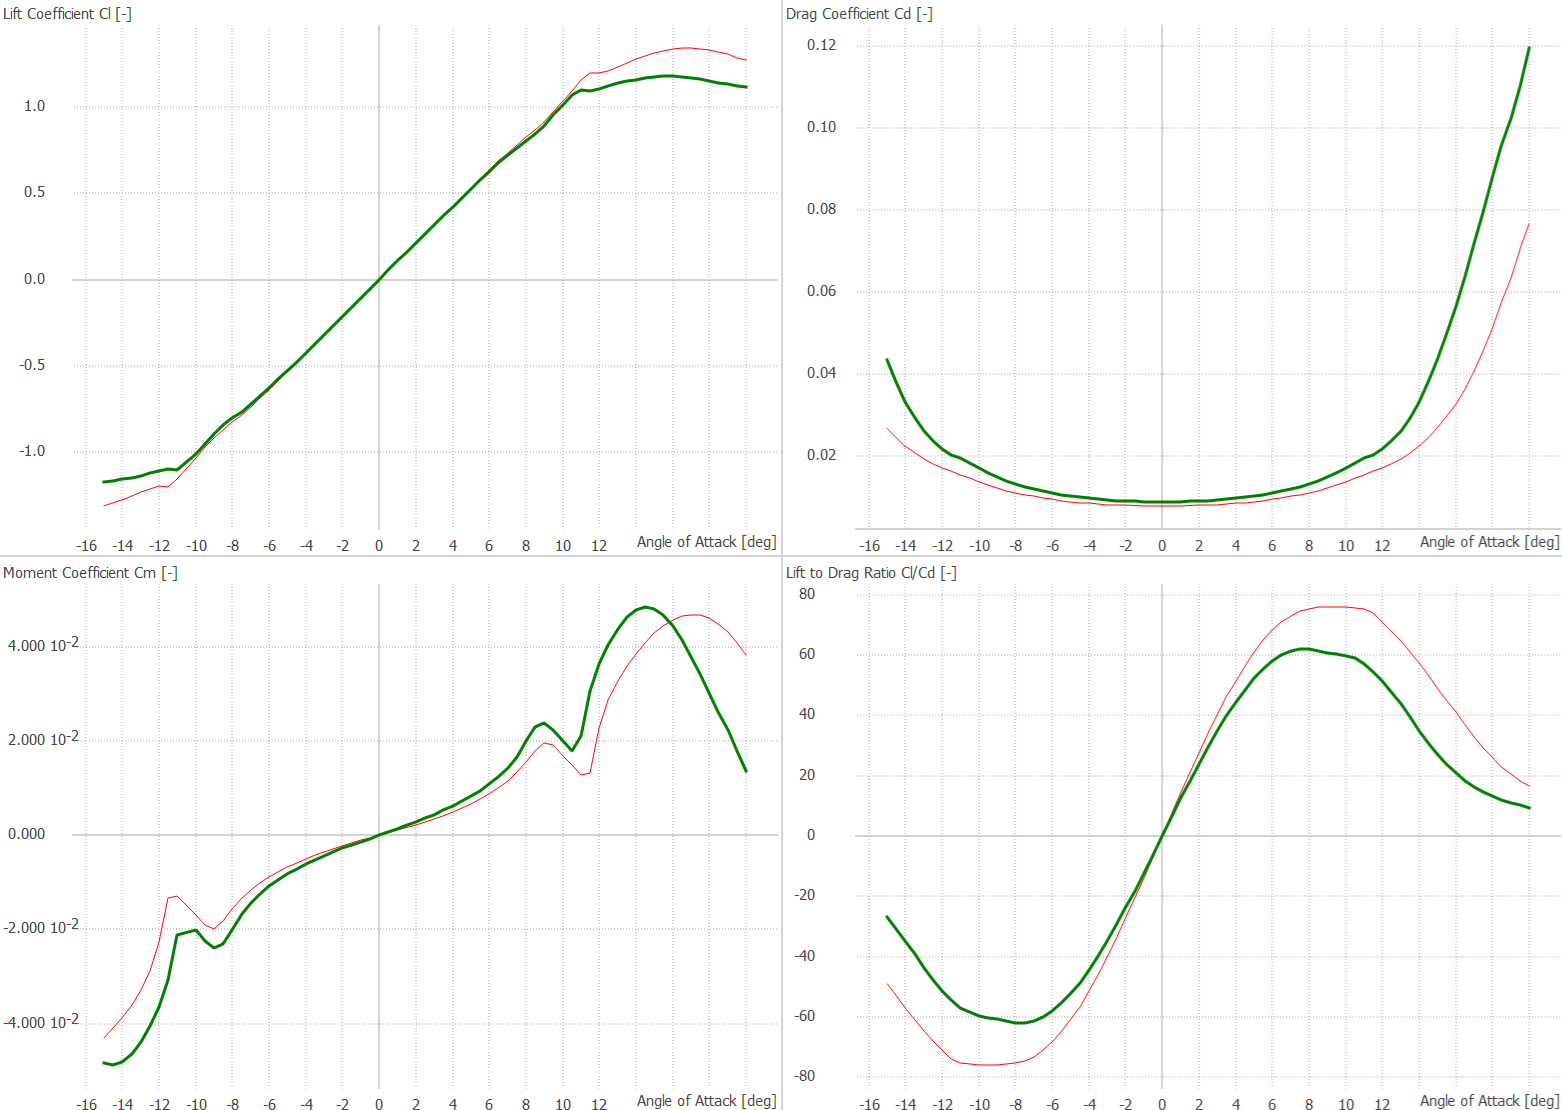
\includegraphics[width=0.92\textwidth]{Figuras/Figuras Antecedentes/qfoil_vs_xfoil.png}
    \caption[Comparación entre QFoil y XFoil para el perfil NACA 0020.]{Comparación entre QFoil (verde) y XFoil (rojo) para el perfil NACA 0020 a $Re = 1 \times 10^6$: coeficientes de sustentación, resistencia y momento, y eficiencia aerodinámica. Tomado de la documentación oficial~\parencite{QBladeDocsQFoil2024}.}
    \label{fig:qfoil_vs_xfoil}
\end{figure}

Esta distinción es relevante en las \gls{vawt}, donde las palas recorren excursiones de ángulo de ataque muy amplias en un solo ciclo de rotación y operan de forma habitual en pérdida profunda. En ese régimen es donde XFoil presenta mayores dificultades de convergencia y donde las diferencias de la Figura~\ref{fig:qfoil_vs_xfoil} se vuelven determinantes, razón por la cual QFoil resulta preferible para el cálculo de polares destinadas a una \gls{vawt}. La propia documentación advierte, no obstante, que QFoil no es numéricamente equivalente a XFoil y que sus resultados deben revalidarse contra datos experimentales antes de emplearse~\parencite{QBladeDocsQFoil2024}. Esa es la comparación pertinente aquí: no XFoil contra QFoil, sino QFoil contra mediciones reales del perfil NACA 0018 en el rango de Reynolds de interés. Los datos experimentales de referencia se presentan en la Sección~\ref{sec:caracterizacion_aero}, y su contraste cuantitativo con las polares de QFoil, que respalda la configuración finalmente adoptada, se muestra en el Capítulo~4 (Figura~\ref{fig:comparacion_ncrit_250k}).

\subsubsection{Parámetros de simulación aerodinámica}

\textbf{Número de Mach ($M$):} Representa la relación entre la velocidad del flujo y la velocidad del sonido, y cuantifica cuánto varía la densidad del aire al acelerarse sobre el perfil. Un flujo se considera incompresible cuando $M < 0{,}3$, umbral bajo el cual la variación de densidad respecto de la condición de reposo se mantiene por debajo del $5\%$ y puede despreciarse~\parencite{Anderson2016}. Los códigos basados en el método de paneles, como XFoil y QFoil, incorporan la corrección de compresibilidad de Kármán-Tsien~\parencite{Karman1941,Tsien1939} para extender su validez a números de Mach mayores; dicha corrección deja de ser fiable cuando el número de Mach local sobre el perfil supera aproximadamente $1{,}05$, condición en que aparecen regiones supersónicas y ondas de choque que el método no resuelve~\parencite{drelaXfoil699}.

En una \gls{vawt} el número de Mach relevante no es el del viento incidente sino el asociado a la velocidad relativa $W$, que combina la velocidad del viento con la velocidad tangencial de la pala y resulta considerablemente mayor. Aun así, al ser la velocidad de punta de una máquina de eje vertical sustancialmente menor que la de una \gls{hawt} de tamaño comparable, estos rotores operan siempre en régimen claramente subsónico y los efectos de compresibilidad resultan despreciables.

\textbf{Parámetro de Transición ($N_{crit}$):} Es el factor principal del modelo de transición $e^N$ utilizado para predecir el cambio natural de la capa límite de régimen laminar a turbulento sobre el perfil alar. El modelo se apoya en que, antes de la transición, las pequeñas perturbaciones presentes en la capa límite laminar (las ondas de Tollmien-Schlichting) se amplifican de forma exponencial al avanzar sobre el perfil. Si $A_0$ es la amplitud de la perturbación más inestable en el punto donde comienza a crecer y $A$ su amplitud en una posición posterior, el factor de amplificación $n$ se define según la Ec.~\ref{eq:en_transicion}:

\begin{equation}
n = \ln\left( \frac{A}{A_0} \right)
\label{eq:en_transicion}
\end{equation}

El criterio supone que la transición ocurre donde $n$ alcanza el valor umbral $N_{crit}$, de modo que este parámetro es el logaritmo del factor de amplificación admisible antes de que el flujo se vuelva turbulento: $N_{crit} = 9$, por ejemplo, corresponde a una amplificación de $e^{9} \approx 8100$ veces~\parencite{drela1989xfoil}. Su valor no es una propiedad del perfil sino del entorno: cuanto mayor sea la turbulencia o la rugosidad del flujo incidente, mayores serán las perturbaciones iniciales y menor la amplificación necesaria para desencadenar la transición, por lo que $N_{crit}$ disminuye. Valores elevados se asocian a flujos libres de perturbaciones, como en planeadores, y valores bajos a entornos de mayor turbulencia; la Tabla~\ref{tab:ncrit_values} recoge los valores de referencia recomendados según las condiciones del flujo.

Su valor tiene un efecto directo sobre las curvas polares del perfil: un $N_{crit}$ elevado retrasa la transición de la capa límite y se traduce en un mayor coeficiente de sustentación máximo ($C_{l,max}$), un ángulo de pérdida más tardío y un coeficiente de arrastre reducido en el rango lineal previo a la pérdida, mientras que valores bajos anticipan la transición turbulenta, reducen el $C_{l,max}$, desplazan la pérdida hacia ángulos de ataque menores e incrementan el arrastre por fricción superficial~\parencite{drela1989xfoil}.

\begin{table}[H]
    \centering
    \caption{Valores de $N_{crit}$ de referencia según la documentación de Xfoil.}
    \label{tab:ncrit_values}
    \begin{tabular}{lc}
        \hline
        \textbf{Condición del Flujo} & \textbf{Valor $N_{crit}$}\\
        \hline
        Soplado en planeador (sailplane)   & 12 -- 14 \\
        Motoplaneador (motorglider)        & 11 -- 13 \\
        Túnel de viento limpio             & 10 -- 12 \\
        Túnel de viento promedio           & 9        \\
        Túnel de viento con turbulencia    & 4 -- 8   \\
        \hline
    \end{tabular}
\end{table}

La física del perfil es sensible al número de Reynolds, especialmente en regímenes bajos y moderados. A $Re$ entre $1 \times 10^6$ y $3 \times 10^6$, es frecuente la formación de una burbuja de separación laminar: la capa límite, todavía laminar, se separa de la superficie antes de haber transicionado a turbulenta, pero la capa de corte ya separada sí transiciona, y esa capa turbulenta, con mayor cantidad de movimiento, logra readherirse aguas abajo. El resultado es una pequeña región cerrada de recirculación entre el punto de separación laminar y el de readherencia turbulenta, distinta de la separación progresiva que avanza desde el borde de fuga descrita en la Sección~\ref{sec:dynamicstall} (Figura~\ref{fig:stall_progresion}). Aunque de extensión pequeña, esta burbuja modifica la presión efectiva sobre el extradós y con ello el coeficiente de sustentación máximo ($C_{l,max}$) y el comportamiento de la pérdida~\parencite{drela1989xfoil}. A números de Reynolds más altos, en cambio, la transición ocurre de forma casi inmediata y la burbuja prácticamente desaparece.

\textbf{Transición Forzada (Forced Transition):} Parámetros que definen la posición exacta (expresada como una fracción de la cuerda, $x/c$) en la cual se fuerza la transición a flujo turbulento en la superficie superior (\textit{Forced Top Transition}) e inferior (\textit{Forced Bottom Transition}) del perfil, anulando el cálculo del modelo de transición natural en dicha zona. Se emplean conceptualmente para simular la presencia de cintas de transición (\textit{trips}) físicas o pérdidas de rendimiento por suciedad y rugosidad acumulada~\parencite{drela1989xfoil}.

La Tabla~\ref{tab:resumen_params_polares} resume los parámetros que gobiernan el cálculo de polares y su efecto sobre los resultados aerodinámicos.

\begin{table}[H]
    \centering
    \caption{Resumen de parámetros que gobiernan el cálculo de polares aerodinámicas.}
    \label{tab:resumen_params_polares}
    \begin{tabular}{lcc}
        \hline
        \textbf{Parámetro} & \textbf{Fenómeno físico} & \textbf{Símbolo} \\
        \hline
        Número de Reynolds & Viscosidad & $Re$ \\
        Número de Mach & Compresibilidad & $M$ \\
        $N_{crit}$ & Transición laminar-turbulenta & $N_{crit}$ \\
        Transición forzada & Fijación artificial de la transición & $x/c$ \\
        \hline
    \end{tabular}
\end{table}

\subsection{Caracterización aerodinámica y datos de validación}
\label{sec:caracterizacion_aero}

Dado que los códigos de cálculo descansan en modelos semiempíricos de la capa límite, sus polares requieren contraste con mediciones. El ensayo de referencia para ello es el túnel de viento, donde el perfil se monta en condiciones bidimensionales y se registran las fuerzas mientras varía el ángulo de ataque.

El estudio de \textcite{Bianchini2015} constituye un antecedente pertinente para la caracterización aerodinámica de perfiles en \gls{vawt}, al obtener las polares definidas en la Sección~\ref{sec:dynamicstall} en el rango completo de $360^\circ$ de ángulo de ataque para el perfil NACA 0018. Los ensayos se realizaron en un túnel de viento de baja turbulencia, con intensidad inferior al $0{,}1\%$, para números de Reynolds entre $6{,}0 \times 10^4$ y $3{,}0 \times 10^5$. Los coeficientes de sustentación y resistencia medidos se contrastan punto a punto con los obtenidos mediante simulaciones de \gls{cfd} (Figura~\ref{fig:comparacion_resultados_paper}), con concordancia general en todo el rango y discrepancias acotadas, explícitamente reportadas por los autores, entre $150^\circ$ y $180^\circ$ para la sustentación y a ángulos positivos elevados para la resistencia, nivel de correspondencia que permite emplear sus polares como referencia para la validación de modelos numéricos. El estudio identificó, asimismo, deficiencias en la base de datos histórica de Sheldahl y Klimas (1981) para este perfil, y concluye que el modelo de Montgomerie ofrece el mejor desempeño entre los métodos de extrapolación evaluados.

\begin{figure}[h]
\centering
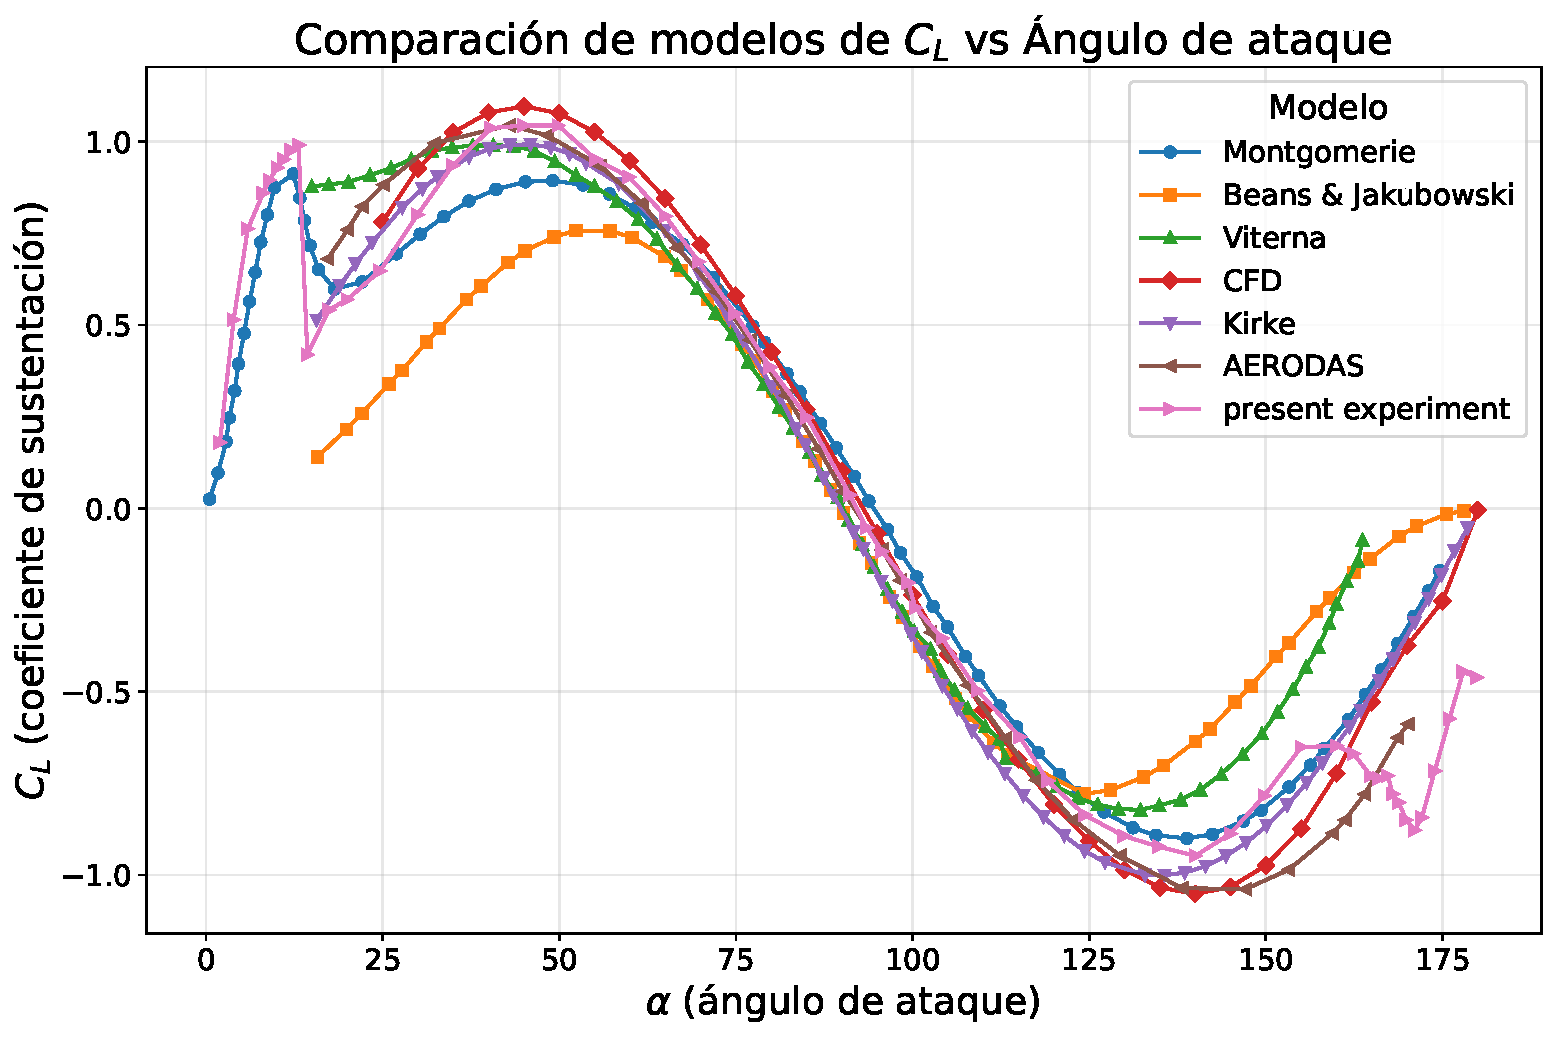
\includegraphics[width=0.8\textwidth]{Figuras/Figuras Antecedentes/LC AoA comparacion.pdf}
\caption{Comparación de polares del perfil NACA 0018 entre modelos de predicción.}
\label{fig:comparacion_resultados_paper}
\end{figure}

\subsection{Extrapolación de polares aerodinámicas}

Debido a que los códigos de cálculo, por la razón expuesta en la Sección~\ref{sec:polares}, dejan de converger una vez que la separación se vuelve masiva, generan polares confiables solo hasta la pérdida y un rango limitado más allá de ella. Como la caracterización del rendimiento aerodinámico de la turbina requiere $C_l$, $C_d$ y $C_m$ definidos en los $360^\circ$ de operación, resulta necesario extender esos datos mediante un modelo de extrapolación.

La literatura ofrece más de uno; se repasan aquí los dos más difundidos, que responden a principios de construcción distintos. El de \textcite{viterna1982theoretical} no describe la física del flujo separado, sino que deduce la forma de la curva imponiendo tres condiciones sobre el tramo posterior a la pérdida: continuidad con la polar adherida en el ángulo de pérdida, un coeficiente de torque constante a lo largo de todo ese tramo, y el valor de arrastre que corresponde a $90^\circ$ según la relación de aspecto de la pala. La segunda condición es la que fija la forma, y proviene de una observación experimental sobre rotores regulados por pérdida, esto es, aquellos que a partir de cierta velocidad de viento operan intencionalmente en pérdida para limitar la potencia captada: en ellos el torque medido más allá de la pérdida resulta prácticamente independiente de la velocidad del viento y, por tanto, del ángulo de ataque. Las expresiones que satisfacen las tres condiciones son las Ecs.~\ref{eq:viterna_cl} y~\ref{eq:viterna_cd}:

\begin{equation}
C_l = A_1 \sin(2\alpha) + A_2 \frac{\cos^2\alpha}{\sin\alpha}
\label{eq:viterna_cl}
\end{equation}
\begin{equation}
C_d = B_1 \sin^2\alpha + B_2 \cos\alpha
\label{eq:viterna_cd}
\end{equation}

donde $A_1$, $A_2$, $B_1$ y $B_2$ quedan completamente determinados por solo cuatro datos del perfil: el ángulo de pérdida $\alpha_s$, los coeficientes $C_{l,s}$ y $C_{d,s}$ en ese ángulo, y la relación de aspecto de la pala $AR = R/c$, que fija el arrastre a $90^\circ$ mediante la correlación empírica $C_{d,90} = 1{,}11 + 0{,}018\,AR$. Fijado el punto de pérdida, la curva completa queda determinada, sin parámetros adicionales para ajustar su forma. Esa rigidez es coherente con el propósito para el que fue concebido, capturar el torque en pérdida frontal de una HAWT, pero no con lo que exige una VAWT: valores físicamente consistentes de $C_l$, $C_d$ y $C_m$ en los $360^\circ$ completos, incluido el flujo inverso, régimen donde la hipótesis que origina el modelo, un torque post-pérdida constante, deja de tener sentido.

El modelo de Montgomerie parte de un principio distinto. En lugar de deducir la curva de una condición sobre el torque, la construye como una mezcla de las dos soluciones límite que sí se conocen: la recta de flujo potencial, válida mientras el flujo permanece adherido, y la curva de placa plana delgada, válida cuando la separación es completa, ponderadas por una función de transición que las une de forma continua en todo el círculo~\parencite{montgomerie2004methods}. Al no imponer condición alguna sobre el torque, la construcción no privilegia ningún tramo de la polar y admite parámetros de ajuste independientes, detallados en la subsección siguiente: además del punto de transición, la amplitud del arrastre en placa plana ($C_{d90}$) y la suavidad con que la curva se aproxima a ese régimen a cada lado ($A^+$, $A^-$, $B^+$, $B^-$). Esa libertad es la que permite reproducir el comportamiento asimétrico de un perfil en pérdida profunda y flujo inverso, y la que \textcite{Bianchini2015} identifican como la razón por la que Montgomerie reproduce mejor sus datos experimentales en el rango completo de $360^\circ$. La Tabla~\ref{tab:extrapolacion_metodos} contrasta ambos principios de construcción.

\begin{table}[H]
    \centering
    \caption[Comparación de los métodos de extrapolación de polares.]{Comparación de los principios de construcción de los métodos de extrapolación de polares. Elaborada a partir de \textcite{viterna1982theoretical}, \textcite{montgomerie2004methods} y \textcite{Bianchini2015}.}
    \label{tab:extrapolacion_metodos}
    \renewcommand{\arraystretch}{1.2}
    \footnotesize
    \begin{tabular}{p{1.9cm} p{4.0cm} p{3.2cm} p{4.2cm}}
        \hline
        \textbf{Método} & \textbf{Principio de construcción} & \textbf{Grados de libertad} & \textbf{Alcance y limitaciones} \\
        \hline
        Viterna &
        Deduce el tramo posterior a la pérdida imponiendo continuidad con la polar adherida, torque constante más allá del ángulo de pérdida y el arrastre que corresponde a $90^\circ$~\parencite{viterna1982theoretical} &
        Ninguno: el punto de pérdida y la relación de aspecto determinan los cuatro coeficientes y, con ellos, toda la curva &
        Concebido para el tramo en pérdida de una HAWT regulada por pérdida; sus expresiones no incorporan parámetros que distingan un lado de la polar del otro, y la hipótesis de torque constante pierde sentido en flujo inverso \\
        Montgomerie &
        Interpola entre la recta de flujo potencial y la curva de placa plana delgada mediante una función de transición continua en todo el círculo~\parencite{montgomerie2004methods} &
        Punto de transición, $C_{d90}$ y los parámetros de acoplamiento $A^{\pm}$ y $B^{\pm}$, ajustables por separado a cada lado de la polar &
        Formulado para el rango completo de $\pm 180^\circ$; exige calibrar esos parámetros contra datos del perfil, y en el contraste experimental sobre el NACA 0018 resultó el de mejor desempeño entre los métodos evaluados~\parencite{Bianchini2015} \\
        \hline
    \end{tabular}
\end{table}

\subsubsection{Modelo Montgomerie y sus parámetros de configuración}

El modelo, desarrollado en la Agencia Sueca de Investigación de Defensa (FOI), formula esa interpolación mediante las expresiones siguientes.

Función de transición ($f$): define el peso relativo entre el régimen de flujo adherido y el separado, según la Ec.~\ref{eq:mont_f}:
\begin{equation}
f = \frac{1}{1 + k \cdot \Delta\alpha^4}
\label{eq:mont_f}
\end{equation}

donde $\alpha$ corresponde al ángulo de ataque; $\Delta\alpha$ es su desplazamiento respecto al punto en que la curva original se aparta de la recta de flujo potencial, esto es, respecto al inicio de la separación, y $k$ es una constante de ajuste que se calibra con dos puntos de la curva dada. Mientras $\alpha$ se mantiene dentro del tramo adherido, $\Delta\alpha \approx 0$ y $f \approx 1$; más allá de ese punto, $\Delta\alpha$ crece y $f$ decae rápidamente hacia $0$, por la potencia cuarta del denominador.

Coeficiente de sustentación ($C_l$): Se obtiene interpolando entre la línea de flujo potencial ($t$) y la curva de placa plana ($s$), según la Ec.~\ref{eq:mont_cl}:
\begin{equation}
C_L = f \cdot t + (1 - f) \cdot s
\label{eq:mont_cl}
\end{equation}

La Figura~\ref{fig:montgomerie_st} ilustra esta interpolación para un perfil simétrico. El panel (a) muestra la forma de $f$, una meseta en $1$ dentro del tramo adherido que cae abruptamente una vez superado el punto de transición $\alpha_M$; el panel (b), las dos curvas que $f$ pondera, la recta $t(\alpha)$ y la curva de placa plana $s(\alpha)$, junto con el resultado de la Ec.~\ref{eq:mont_cl}: mientras $f \approx 1$, $C_l$ coincide con la recta $t$; una vez que $f$ cae, converge hacia la curva acotada $s$, evitando que la recta, que de otro modo crecería sin límite, se extienda a ángulos donde ya no representa flujo adherido.

\begin{figure}[H]
    \centering
    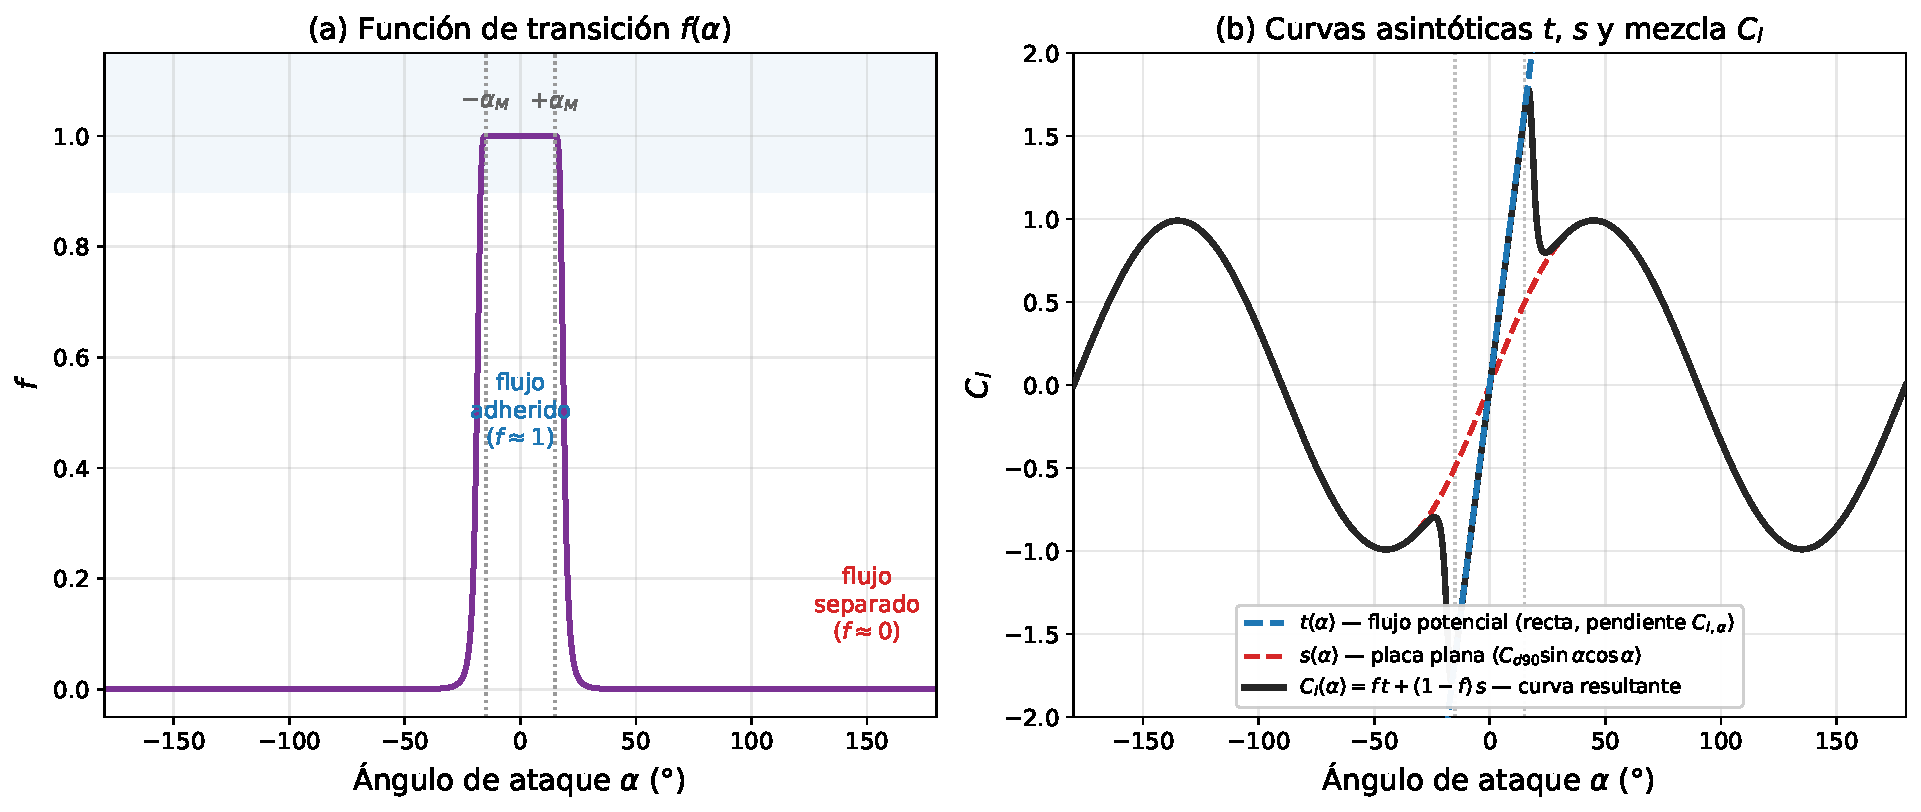
\includegraphics[width=0.95\textwidth]{Figuras/Figuras Antecedentes/montgomerie_st.pdf}
    \caption[Función de transición e interpolación entre flujo potencial y placa plana en el modelo de Montgomerie.]{Ilustración del modelo de Montgomerie para un perfil simétrico: (a) función de transición $f(\alpha)$ y (b) curvas de flujo potencial $t(\alpha)$, placa plana $s(\alpha)$ y sustentación resultante $C_l(\alpha)$.}
    \label{fig:montgomerie_st}
\end{figure}

Coeficiente de arrastre ($C_d$): queda fijado por el parámetro $C_{d90}$, el coeficiente de resistencia del perfil a $\alpha = 90^\circ$, esto es, cuando se comporta como una placa plana orientada perpendicularmente al flujo, valor que define la amplitud de toda la curva de arrastre en régimen separado según la Ec.~\ref{eq:mont_cd}:
\begin{equation}
C_{D, thinPlate} = C_{d90} \cdot \sin^2(\alpha)
\label{eq:mont_cd}
\end{equation}

Coeficiente de momento ($C_m$): se calcula utilizando un brazo de momento variable que asegura el realismo físico del punto de aplicación de la fuerza en pérdida profunda.

A diferencia del arrastre a $90^\circ$, que fija solo la amplitud de la curva de placa plana, los parámetros de acoplamiento $A^+$, $A^-$, $B^+$ y $B^-$ controlan la forma y la suavidad con que la curva transiciona hacia ese régimen en cada lado de la polar, para ángulos positivos y negativos respectivamente. Este conjunto, ausente en modelos más rígidos como el de Viterna, es el que permite reproducir curvas asimétricas o con transiciones de distinta suavidad a cada lado del punto de pérdida.

Estos parámetros, junto con la pendiente de sustentación determinada a partir de las curvas polares, definen la configuración del modelo de Montgomerie.

\section{Análisis estructural y criterios de falla}
\label{sec:analisis-estructural}

Una pala de aerogenerador es, estructuralmente, una viga sometida a solicitaciones de naturaleza distinta. Las cargas aerodinámicas, generadas por la interacción del perfil con el flujo incidente, varían continuamente en el tiempo; las inerciales, esto es, la gravitatoria y la centrífuga, se mantienen estacionarias mientras la velocidad de rotación no cambia~\parencite{Galinos2015}. En un H-rotor, cuyas palas rectas son paralelas al eje de rotación, la fuerza centrífuga actúa en dirección perpendicular a la envergadura, según se describió en la Sección~\ref{sec:vtip}. Las uniones a los struts constituyen los apoyos de la pala, de modo que esta flecta en el vano comprendido entre ellas y en los tramos que quedan en voladizo hacia las puntas. Verificar la pala consiste, en esencia, en traducir esas solicitaciones en un estado de tensiones y deformaciones dentro del material, y contrastarlo con lo que el material admite: su resistencia frente a la carga máxima, su estabilidad frente al pandeo y su capacidad de soportar la repetición de ciclos a lo largo de la vida útil.

\subsection{Configuración estructural de una pala}

Antes de discutir materiales conviene fijar la nomenclatura de los elementos que componen una pala, ya que de ellos depende cómo se reparten las tensiones. La sección transversal se organiza en dos partes con funciones distintas, según se ilustra en la Figura~\ref{fig:estructura_pala}: el contorno aerodinámico, formado por pieles relativamente delgadas que definen la forma del perfil pero no están dimensionadas para tomar por sí solas la flexión, y un elemento longitudinal interno en que estas se apoyan, un larguero o un conjunto de almas, que recorre la envergadura y absorbe una parte sustancial de la carga~\parencite{Brondsted2005}.

\begin{figure}[H]
    \centering
    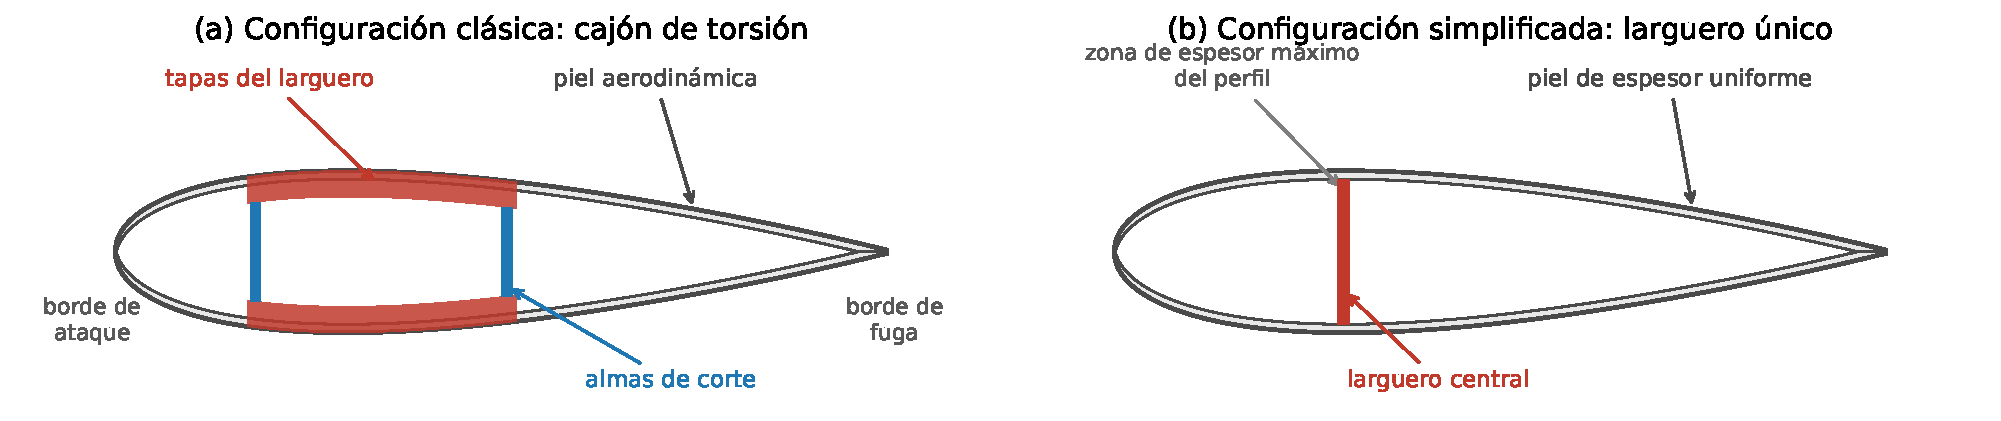
\includegraphics[width=\textwidth]{Figuras/Figuras Antecedentes/estructura_pala.pdf}
    \caption[Elementos estructurales de una pala de aerogenerador en sección transversal.]{Elementos estructurales de una pala de aerogenerador en sección transversal, en dos configuraciones habituales. Nomenclatura según la sección de referencia descrita por \textcite{Brondsted2005}.}
    \label{fig:estructura_pala}
\end{figure}

El reparto de funciones sigue una lógica sencilla. Al flexionarse la pala, las tensiones normales de tracción y compresión se concentran en las caras superior e inferior, las más alejadas del eje neutro, esto es, de la línea de la sección que no se alarga ni se acorta al flectar y que, por tanto, no está sometida a tensión; por eso la configuración clásica de las palas de gran tamaño (Figura~\ref{fig:estructura_pala}a) engrosa el laminado precisamente allí, formando las \textit{tapas del larguero}, y las une mediante una o dos \textit{almas de corte}, elementos verticales que transmiten el esfuerzo cortante y evitan que las tapas se desplacen una respecto de la otra. El conjunto constituye un cajón de torsión que aporta la rigidez a flexión y a torsión de la pala. En palas rectas de menor tamaño resulta habitual una configuración más simple (Figura~\ref{fig:estructura_pala}b), con piel de espesor prácticamente uniforme y un único larguero situado en la zona de espesor máximo del perfil, donde el brazo respecto del eje neutro es mayor. Los extremos de la sección reciben nombres propios: el \textit{borde de ataque}, redondeado, y el \textit{borde de fuga}, afilado, que por su geometría delgada aporta poco a la rigidez y suele ser una zona crítica de fabricación.

Esta arquitectura explica por qué la piel, además de resistencia, requiere estabilidad: los paneles entre elementos de apoyo trabajan en compresión en la cara comprimida de la pala y pueden fallar por pandeo local, es decir, por abolladura, antes de alcanzar la resistencia del material, de modo que el dimensionamiento no depende solo de cuánta tensión soporta el laminado, sino también de la distancia entre elementos rigidizadores.

\subsection{Materiales empleados en palas de aerogeneradores}
\label{sec:materiales_palas}

La selección de material para una pala responde a tres requisitos simultáneos: rigidez elevada, para mantener las deflexiones acotadas y preservar la forma aerodinámica; densidad baja, ya que la propia masa de la pala genera cargas inerciales y gravitatorias; y buen comportamiento a fatiga, dado que la pala acumula del orden de $10^8$ a $10^9$ ciclos durante su vida útil~\parencite{Brondsted2005}. Estos requisitos compiten entre sí, y su compromiso se resume en un índice de mérito que para una viga en flexión vale $M_b = E^{1/2}/\rho$, donde $E$ es el módulo elástico y $\rho$ la densidad: cuanto mayor sea $M_b$, mayor rigidez se obtiene por unidad de masa. Aplicado sobre el conjunto de los materiales de ingeniería, este criterio descarta a la mayoría y, junto con la condición adicional de un módulo absoluto del orden de $10$ a $20$~GPa para limitar las deflexiones, deja como candidatos a los materiales compuestos~\parencite{Brondsted2005}.

La Tabla~\ref{tab:materiales_palas} recoge las propiedades de las fibras candidatas y de los laminados que resultan de combinarlas con una matriz polimérica, esto es, la resina que envuelve las fibras y las solidariza entre sí para que trabajen en conjunto. La fibra de vidrio tipo E ofrece una combinación equilibrada de rigidez moderada, resistencia alta y densidad moderada, a un costo sustancialmente menor, lo que lo ha mantenido como la fibra más utilizada. El carbono casi cuadruplica el módulo del laminado y reduce su densidad, con lo que su índice de mérito resulta unas tres veces superior; su adopción creciente responde tanto al aumento de tamaño de las palas, donde el peso propio se vuelve limitante, como a la caída de su precio~\parencite{Brondsted2005}. Las fibras de aramida, polietileno y celulosa presentan índices de mérito intermedios y densidades bajas, pero ninguna ha alcanzado un desarrollo industrial que las haga viables en palas de gran tamaño.

\begin{table}[H]
    \centering
    \caption[Propiedades de fibras y laminados candidatos para palas de aerogeneradores.]{Propiedades de fibras y laminados candidatos para palas de aerogeneradores. Los laminados corresponden a fibras alineadas en matriz polimérica, con una proporción de fibra del $50\%$ en volumen. Adaptada de \textcite{Brondsted2005}.}
    \label{tab:materiales_palas}
    \renewcommand{\arraystretch}{1.2}
    \footnotesize
    \begin{tabular}{l c c c c c c c}
        \hline
        & \multicolumn{3}{c}{\textbf{Fibra}} & \multicolumn{4}{c}{\textbf{Laminado}} \\
        \cmidrule(lr){2-4} \cmidrule(lr){5-8}
        \textbf{Fibra} & $E_f$ & $\sigma_f$ & $\rho_f$ & $E_c$ & $\sigma_c$ & $\rho_c$ & $E_c^{1/2}/\rho_c$ \\
        & (GPa) & (MPa) & (g/cm$^3$) & (GPa) & (MPa) & (g/cm$^3$) & \\
        \hline
        Vidrio tipo E & 72  & 3500 & 2{,}54 & 38  & 1800 & 1{,}87 & 3{,}3 \\
        Carbono      & 350 & 4000 & 1{,}77 & 176 & 2050 & 1{,}49 & 8{,}9 \\
        Aramida      & 120 & 3600 & 1{,}45 & 61  & 1850 & 1{,}33 & 5{,}9 \\
        Polietileno  & 117 & 2600 & 0{,}97 & 60  & 1350 & 1{,}09 & 7{,}1 \\
        Celulosa     & 80  & 1000 & 1{,}50 & 41  & 550  & 1{,}35 & 4{,}7 \\
        \hline
    \end{tabular}
\end{table}

La pala del caso de estudio ya está definida por el fabricante: se trata de un polímero reforzado con fibra de vidrio (GFRP) con tejido bidireccional a $\pm 45^\circ$, fabricado por infusión al vacío, técnica que permite obtener fracciones volumétricas de fibra elevadas con baja porosidad.

\subsection{Comportamiento mecánico del laminado y criterios de falla}
\label{sec:comportamiento_laminado}

Dos rasgos del comportamiento de un compuesto de fibra de vidrio condicionan la forma en que se verifica la pala. El primero es que se trata de un material \textit{frágil}, es decir, a diferencia de un material dúctil, que fluye plásticamente y redistribuye tensiones antes de romper, el laminado responde de forma prácticamente lineal hasta la rotura cuando la carga la toman las fibras, sin una meseta de fluencia que advierta la proximidad del fallo, y la rotura sobreviene por fractura frágil de las fibras y de la matriz que las envuelve~\parencite{Huh2012,Moraras2023}. La Figura~\ref{fig:curva_esfuerzo_deformacion} recoge esa respuesta para el material de la pala del caso de estudio. Esa linealidad simplifica el análisis, pues permite tratar la respuesta como proporcional a la carga, pero elimina el margen de aviso que ofrece la plastificación y obliga a apoyarse en los factores parciales de seguridad para cubrir la incertidumbre.

El segundo rasgo es la \textit{ortotropía}: las propiedades del laminado dependen de la dirección, con valores máximos en la dirección de las fibras y sustancialmente menores en la transversal y en corte, donde la carga la toma principalmente la matriz. La rigidez decae de forma continua a medida que el ángulo entre la fibra y la carga crece de $0^\circ$ a $90^\circ$~\parencite{Brondsted2005,Huh2012}. Los ensayos sobre laminados de pala miden ese efecto: en placas de fibra de vidrio con tejido a $0^\circ/90^\circ$, la resistencia obtenida al cargar a $45^\circ$ respecto de las fibras cae por debajo de un tercio de la medida en la dirección de estas~\parencite{Moraras2023}, y la mayor resistencia a tracción corresponde a la dirección longitudinal, la de alineación de las fibras~\parencite{Ahmed2021}. Un mismo estado de carga puede ser entonces inofensivo o crítico según cómo esté orientado respecto de las fibras, de modo que no basta con conocer su magnitud y se requiere además la distribución espacial del estado tensional. Esa es la razón de fondo por la que la verificación no puede resolverse con un modelo unidimensional de viga, a lo que se suma que, en las conexiones con los struts, la hipótesis de secciones planas deja de ser válida, ya que las cargas concentradas generan distribuciones de tensión que un modelo de viga no resuelve.

Conviene anticipar aquí hasta dónde llega la verificación que este trabajo realiza con esa base. Aprovechar plenamente la ortotropía exige un criterio de fallo direccional aplicado capa a capa, del tipo de los de Puck o Tsai-Wu, y para eso hace falta conocer la secuencia de apilamiento del laminado, las orientaciones de cada capa y sus resistencias en las direcciones principales del material. El fabricante entrega, en cambio, un único módulo elástico, un coeficiente de Poisson y una resistencia, esto es, un conjunto de propiedades isótropas equivalentes (Sección~\ref{sec:material_pala}). Con esa información el criterio aplicable es el de máxima tensión principal sobre un material isótropo equivalente, que es el que se adopta, y cuyo alcance se retoma al declarar las limitaciones del estudio. La discusión anterior conserva su pertinencia porque identifica qué caracterización del material sería necesaria para cerrar la verificación en los términos que la norma específica de palas contempla.

La rotura de un laminado no ocurre por un único mecanismo. Las imperfecciones que deja el proceso de fabricación dan origen a la fractura de fibras, al agrietamiento de la matriz y a la falla de la interfaz entre ambas, mecanismos elementales que a su vez alimentan el micropandeo de las fibras, la propagación de grietas a través de las capas y la delaminación, esto es, la separación entre capas contiguas~\parencite{Brondsted2005}. Cuál de ellos predomina en fatiga depende del nivel de solicitación: bajo cargas altas gobierna la falla de fibras; a niveles intermedios, la combinación de matriz e interfaz; y bajo cargas bajas, el agrietamiento de la matriz~\parencite{Brondsted2005}.

Ese daño no aparece en el instante de la rotura, sino que se acumula bajo carga mucho antes de ella: el agrietamiento de la matriz progresa hasta incorporar delaminación antes del fallo final~\parencite{Samborsky2010}. En las capas orientadas a $\pm 45^\circ$ las grietas siguen la dirección de las fibras y forman el patrón cruzado de la Figura~\ref{fig:grietas_45}. Su avance no produce una señal visible desde el exterior, de modo que resulta difícil de detectar antes de que comprometa la capacidad del laminado.

\begin{figure}[H]
    \centering
    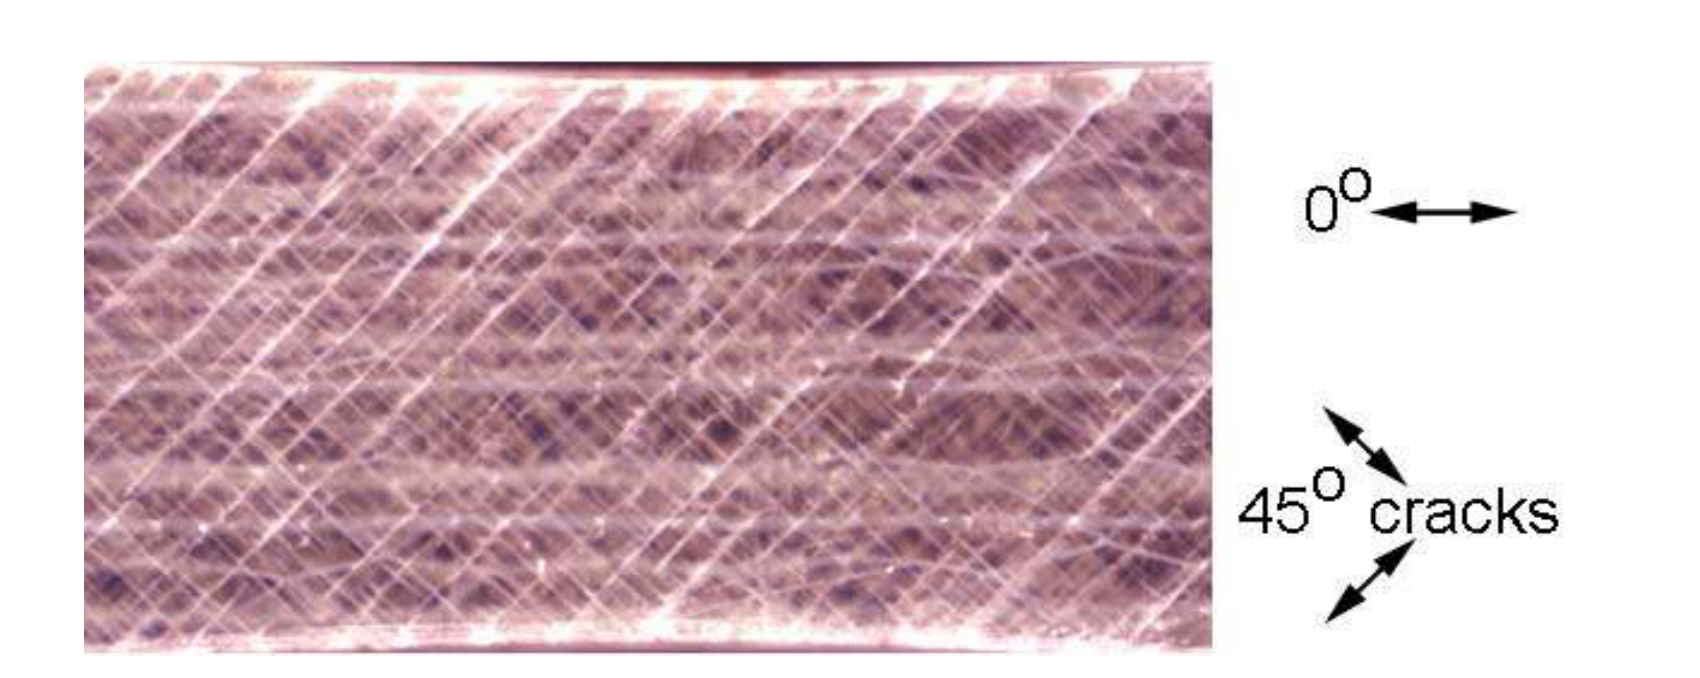
\includegraphics[width=0.75\textwidth]{Figuras/Figuras Antecedentes/grietas_45.png}
    \caption[Agrietamiento de la matriz en capas a $\pm 45^\circ$ antes de la rotura.]{Agrietamiento de la matriz siguiendo la dirección de las fibras en las capas a $\pm 45^\circ$ de un laminado de vidrio, registrado antes de la rotura total de la probeta. La flecha superior indica la dirección de la carga aplicada. Tomado de~\textcite{Samborsky2010}.}
    \label{fig:grietas_45}
\end{figure}

De todos ellos, la delaminación es la que más condiciona la capacidad del laminado, porque se desarrolla entre capas y responde a tensiones interlaminares, cuya evaluación exige representar el laminado capa a capa.

La norma específica de palas traduce esa complejidad en un sistema de factores parciales de material considerablemente más detallado que el de la norma general. Su Sección 6.6.4.2 establece un factor base y lo compone como el producto de una serie de términos que cubren, por separado, el efecto de la temperatura y de la humedad sobre las propiedades, el origen de los datos del material, la validación del cálculo de deformaciones y el número de direcciones de carga consideradas~\parencite{IEC61400-5}. La verificación queda así condicionada no solo por el estado tensional que alcanza la pala, sino también por la calidad de la información disponible sobre el material y sobre el propio modelo de cálculo, aspecto que se retoma al establecer los factores adoptados en este trabajo.

La fragilidad y la ortotropía del laminado explican que la verificación estructural de palas se aborde habitualmente mediante el método de elementos finitos (\gls{fem}). \textcite{HAND2021} lo emplean para verificar la pala compuesta de una \gls{vawt} offshore bajo su caso de carga crítico, contrastando el modelo de elementos finitos con un modelo analítico de viga, y \textcite{Algolfat2022} lo aplican al estudio de la respuesta dinámica de palas de gran escala. El método divide la geometría continua de la pala en un gran número de porciones pequeñas, los elementos, conectadas entre sí en puntos llamados nodos, y supone que dentro de cada elemento los desplazamientos varían según una función sencilla, con lo que el problema continuo, gobernado por ecuaciones diferenciales que no admiten solución analítica en una geometría de esta complejidad, se transforma en un sistema de ecuaciones algebraicas cuyas incógnitas son los desplazamientos nodales. Resuelto ese sistema, se obtienen las deformaciones y, a partir de la ley constitutiva del material, las tensiones en todo el dominio. Dado que la solución es aproximada y mejora al refinar la malla, todo análisis por elementos finitos exige verificar que los resultados ya no dependan significativamente del tamaño de los elementos empleados.

\subsection{Estabilidad estructural y pandeo lineal}
\label{sec:pandeo_teoria}

La resistencia del laminado no agota la verificación estructural. Como se anticipó en la Sección~\ref{sec:analisis-estructural}, la piel de la pala es un cascarón de pared delgada cuyos paneles trabajan en compresión en una de las caras, y un panel comprimido puede perder su forma de equilibrio y abollarse antes de que el material alcance su resistencia. La norma trata esta condición como un estado límite propio, ya que su Sección 7.6.4 exige que las partes portantes de los componentes que no admiten falla no pandeen bajo la carga de diseño, y que ningún componente pandee bajo la carga característica~\parencite{IEC61400-1}.

La carga a la que un panel se vuelve inestable no depende solo del material, sino sobre todo de su geometría. Para una placa comprimida, la tensión crítica sigue la forma de la Ec.~\ref{eq:pandeo_placa}:

\begin{equation}
    \sigma_{cr} = k \, \frac{\pi^2 E}{12\left(1 - \nu^2\right)} \left(\frac{t}{b}\right)^2
    \label{eq:pandeo_placa}
\end{equation}

donde $t$ es el espesor de la placa, $b$ su ancho no apoyado, $E$ el módulo elástico, $\nu$ el coeficiente de Poisson y $k$ un coeficiente que depende de las condiciones de borde y de la relación de aspecto~\parencite{Timoshenko1961}. La dependencia con el cuadrado de la razón $t/b$ explica por qué la estabilidad de la piel se gobierna tanto engrosándola como acortando la distancia entre los elementos que la sostienen, y por qué un rigidizador que no reduce el ancho no apoyado de un panel no mejora su capacidad.

En una geometría real, con paneles de forma irregular y condiciones de borde que no responden a un caso tabulado, la carga crítica se obtiene numéricamente. El planteamiento habitual es el pandeo lineal por autovalores, que parte de la solución estática bajo las cargas aplicadas y busca el factor por el que habría que amplificarlas para que la rigidez del conjunto se anule, según la Ec.~\ref{eq:pandeo_autovalores}:

\begin{equation}
    \left( \left[ K \right] + LM \left[ K_{\sigma} \right] \right) \{\phi\} = \{0\}
    \label{eq:pandeo_autovalores}
\end{equation}

donde $[K]$ es la matriz de rigidez elástica, $[K_{\sigma}]$ la matriz de rigidez geométrica que induce el estado tensional de la solución estática, $\{\phi\}$ el modo de pandeo y $LM$ el multiplicador de carga asociado a ese modo. Un $LM$ mayor que la unidad indica que la estructura no pandea bajo las cargas aplicadas, y su valor mide cuánto margen queda antes de la inestabilidad. El análisis entrega un conjunto de modos ordenados por multiplicador creciente, de los cuales el primero define la condición gobernante. Este enfoque es el que se emplea habitualmente en la verificación de palas de aerogenerador por elementos finitos~\parencite{Boudounit2020,Hameed2015}.

La norma específica de palas admite de forma expresa este planteamiento. Su Sección 6.6.5.6 establece que, cuando la verificación se realiza mediante métodos lineales de análisis de pandeo, debe demostrarse que el autovalor mínimo correspondiente a la primera forma modal supera el factor de seguridad combinado que corresponda~\parencite{IEC61400-5}. Incorpora además una exigencia sobre la discretización que conviene destacar, ya que la idoneidad de la malla ha de acreditarse mediante un estudio de convergencia sobre el propio autovalor de pandeo, y no sobre la tensión, considerándose suficiente cuando aquel no varía más de un $5\%$ al duplicar la densidad de malla en la región pertinente al modo examinado~\parencite{IEC61400-5}. La distinción no es formal, puesto que una malla que ha convergido en tensión puede no haberlo hecho en el autovalor, magnitud considerablemente más sensible a la resolución con que se representa la flexión local del panel.

Conviene retener una limitación del método, ya que la formulación lineal supone que el comportamiento previo a la inestabilidad es elástico y no incorpora imperfecciones geométricas ni la reducción de rigidez que produce el daño progresivo, factores a los que los cascarones de pared delgada son especialmente sensibles. Sus resultados constituyen, por ello, una cota superior de la carga crítica real~\parencite{Timoshenko1961}.

El capítulo siguiente desarrolla el procedimiento con que los elementos revisados, condiciones de viento, simulación aerodinámica y análisis estructural, se aplican al caso de estudio.
